\documentclass{article}
\usepackage{arxiv}
\usepackage[utf8]{inputenc} % allow utf-8 input
\usepackage[T1]{fontenc}    % use 8-bit T1 fonts
\usepackage{hyperref}       % hyperlinks
\usepackage{url}            % simple URL typesetting
\usepackage{booktabs}       % professional-quality tables
\usepackage{amsfonts}       % blackboard math symbols
\usepackage{nicefrac}       % compact symbols for 1/2, etc.
\usepackage{microtype}      % microtypography
\usepackage{lipsum}
% The preceding line is only needed to identify funding in the first footnote. If that is unneeded, please comment it out.
\usepackage{cite}
\usepackage{amsmath,amssymb,amsfonts}
\usepackage{algorithmic}
\usepackage{graphicx}
\usepackage{textcomp}
\usepackage{multirow}
\usepackage{xcolor}
\usepackage{wrapfig}
\def\BibTeX{{\rm B\kern-.05em{\sc i\kern-.025em b}\kern-.08em
    T\kern-.1667em\lower.7ex\hbox{E}\kern-.125emX}}
\DeclareMathOperator{\E}{\mathbb{E}}
\DeclareMathOperator{\R}{\mathbb{R}}
\DeclareMathOperator{\N}{\mathbb{N}}
\DeclareMathOperator{\Q}{\mathbb{Q}}
\DeclareMathOperator{\M}{\mathcal{M}}
\DeclareMathOperator{\Cov}{Cov}

\DeclareMathOperator{\HNG}{\mathcal{M}^{HNG}}
\DeclareMathOperator*{\argmin}{argmin}
\renewcommand{\labelenumi}{\roman{enumi}.}
\newcommand{\ts}{\textsuperscript}

\title{A Deep Learning Approach for pricing Options \\ based on Heston-Nandi-GARCH  \\ \vspace{.38cm} {\footnotesize Supervised by Dr. Lyudmila Grigoryeva \\ \vspace{.38cm} This paper was developed within the Seminar "Deep Learning and Econometrics" \\ at the University of Konstanz, summer term 2019.}}

\author{
  Henrik Brautmeier \\
  Student ID: 905387 \\
  \texttt{henrik.brautmeier@uni.kn} \\
  %% examples of more authors
   \And
 Lukas Wuertenberger \\
 Student ID: 905804 \\
 \texttt{lukas.wuertenberger@uni.kn} \\
}

\begin{document}
\maketitle
\begin{abstract}
We present a continued development of the neural network calibration method by Horvath et al.\cite{Blanka}. We show that their implementation of learning option prices and calibration of model parameters works for the  discrete-time Heston-Nandi-GARCH model, too. Thereby the choice of Heston-Nandi-GARCH model parameters is crucial for the performance of that approach. This seminar paper includes a great variety of performance tests with different datasets and a differentiation between option prices and implied volatilities. We also make suggestions to incorporate market data. Robustness checks cover i.a. a performance comparison to Black Scholes and therefore ensure valid results.
\end{abstract}
\keywords{Deep Learning, , Option Pricing, Heston Nandi, Volatility Modeling} 

%\vspace{3cm}

\textit{\textbf{Acknowledgments}} Special thanks to Lyudmila Grigoryeva for her universal support as well as her target-oriented criticism. We are grateful to Juan-Pablo Ortega for his stimulating input.
%\begin{center}
%\textbf{Acknowledgments}\\
%Special thanks to Lyudmila Gregorieva for her universal support as well as her target-oriented criticism.\\ We are grateful to Juan-Pablo Ortega for his stimulating input.\end{center}

\newpage \tableofcontents\newpage
\section{Introduction}
Since the first occurrence of modern derivatives end of last century, their importance increased significantly. Besides the usage as additional investment opportunity, options and other derivatives provide an utmost important tool for controlling market risk. Hence, researches have spend years investigating pricing and hedging of such financial products. Starting with the work of Black and Scholes (1973) and Merton (1973), tons of market models were introduced and analysed, each with it's own upsides and flaws. With increasing complexity, it's not possible to ensure the existence of closed form pricing formulas. Therefore calibrating models and estimating optimal parameters lead to the necessity of very computation-intensive simulations, which themselves add approximation errors to each calculation. This explains the attractiveness of the Black-Scholes-Merton model even after more realistic stochastic pricing models have been developed.  \\ 
To tackle these problems, Horvath et al  \cite{Blanka} introduce a new approach. The authors provide a method on separating pricing and calibration process using feed-forward neutral networks. Firstly, a neural net is trained to map model parameters directly to the pricing surface. By doing so the computational-intensive simulations are needed  only once for training. Afterwards the neural net  can be used as fast and accurate pricing function. Secondly, the calibration task is reduced to a "simple" constrained optimization task. The trained net is used as input function and no further computation meaningful steps are needed. \\
Using continuous-time stochastic volatility models often results in problems when one is asked not only to calibrate a model to observable market data, but to fit historical observations or future projections. In this paper we use the approach of \cite{Blanka} and apply it to discrete-time models, namely Heston-Nandi-GARCH. This allows to price in a real world scenario and not only under a risk-neutral markets. One advantage of using Heston and Nandi's model is the existence of a closed form solution. Hence, we do not deal with additional approximation errors resulting from Monte-Carlo simulation. Nonetheless, this approach is easily generalizable to any other discrete-time model. Furthermore we provide a rudimentary way on involving real data into the setting by combining the deep learning model with standard econometric theory.



\section{Recap: The GARCH-Model of Heston and Nandi}\label{sec:HNG}
This paper will use the market model developed by Heston and Nandi \cite{HestonNandi}. Therefore a short recap of the most important properties is necessary. \\
The development of a pricing model for European style options by Black, Scholes (1973) and Merton (1973) was crucial for the analysis and hedging of such assets. However, the simple structure does not reflect the behaviour of modern financial markets. Neither normal distributed returns nor a time invariant volatility can be observed in modern financial markets. While the Black-Scholes-Merton model (BS model) implies a flat volatility surface, real volatility surfaces tend to depend on the time to maturity as well as the strike of an option. To account for the complex structure of the underlying volatility process researchers developed a variety of different solutions. Engle's generalized autoregressive  conditional heteroscedasticity (GARCH) models  proved helpful and reasonable in an economic setting (cf. Engle \cite{EngleGARCH}). \\
In their work \cite{HestonNandi97} in 1997 and \cite{HestonNandi} in 2000 Heston and Nandi presented a discrete model  preserving the structure of Black and Scholes, while tackling previously mentioned problems by modeling the volatility via GARCH processes (henceforth HNG model). Heston and Nandi point out that in comparison to continuous-time stochastic volatility models, which are not observable,  a GARCH structure provides the possibility to use historic prices of the underlying for estimations.\\
The following assumptions are made in the HNG model. First, a time-discrete market on equidistant grid with \mbox{$\Delta t = 1$} is considered. Secondly, the yearly risk-free rate $r$ is constant and discount rates are continuously compounded.
Third, the underlying assets price $S_t$ follows the dynamic of \eqref{eq:HNG}
\begin{align}
\begin{cases}
Y_t&=\ln(S_t)-\ln(S_{t-1}) =r+\lambda h_t+\sqrt{h_t}z_t\\
    h_t &= \omega+\sum\limits_{i=1}^q \alpha_i \left( z_{t-1}-\gamma_i \sqrt{h_{t-1}}\right)^2+\sum\limits_{i=1}^p\beta_i h_{t-1}\\
S_0&=s\in \R^+\\
h_0&=\eta\in \R^+\label{eq:HNG}
\end{cases}
\end{align}
where $z_t\overset{iid}{\sim} N(0,1),\omega,\alpha_i,\beta_i,\gamma_i,\lambda\in\R$ and $p,q\in\N$.\\ Previous research (cf. \cite{GARCH}) indicate that the case of $p=q=1$ is sufficient and therefore will be considered in this paper. Similar to Engle's GARCH(1,1) process the volatility $(h_t)_t$ is weakly stationary iff  $|\alpha\gamma^2+\beta|<1$. Positivity can be assured by assuming $\alpha\geq 0$, $\beta\geq 0$ and $\omega >0$. It is easy to derive the long term expectation of the volatility $(h_t)_t$ under stationarity:
\begin{align*}
    \E(h_t)= \frac{\omega+\alpha}{1-\alpha \gamma^2-\beta}
\end{align*}
In addition to Engle's GARCH Heston and Nandi account for leverage effects via the skewness parameter $\gamma$. The conditional covariance between $Y_t$ and $h_t$ is 
\[\Cov(h_{t+1},\ln(S_t)|\mathcal{F}_{t-1})=-2\alpha\gamma h_t.\]
As usual $(\mathcal{F}_t)_t$ denotes the filtration generated by $(S_t)_t$. A positive $\gamma$ leads to a leverage effect. \\
Heston and Nandi show that the corresponding risk-neutral process has an identical GARCH form as \eqref{eq:HNG} with replacing $\lambda$ by $\lambda^*=-\frac{1}{2}$ and $\gamma$ by $\gamma^*=\lambda+\gamma+\frac{1}{2}$. This results in the following risk-neutral model:
\begin{align*}
\begin{cases}
Y_t&=\ln(S_t)-\ln(S_{t-1}) =r-\frac{1}{2}h_t+\sqrt{h_t}z^*_t\\
    h_t &= \omega+\alpha \left( z^*_{t-1}-\gamma^* \sqrt{h_{t-1}}\right)^2+\beta h_{t-1}\\
S_0&=s\in \R^+\\
h_0&=\eta\in \R^+\
\end{cases}
\end{align*}
where $z^*_t\overset{iid}{\sim} N(0,1)$ but only under the risk neutral measure $\Q$\footnote{Even if the assumption of $z_t\overset{iid}{\sim} N(0,1)$ is released, the model still works. But the value of a call option cannot be calculated via Black-Scholes formula. In this case formula \eqref{eq:pricing} does not hold. Furthermore only pseudo Maximum Likelihood estimation is possible in Section \ref{sec:real_data}.}.\\
This change in measure has two important implications. The expected return of the underlying is, similar to BS, equal to the risk-free rate $r$ and, given a positive $\lambda$, it holds $\gamma<\gamma^*$. This implies that in risk-neutral setting a higher average volatility  and  a stronger degree of leverage is observed. A more detailed analysis can be found in chapter 4.2 of \cite{Book}. \\
Under the risk-neutral measure $\Q$ the price $C$ of an European call option with Strike $K$ at time $t$ and expiration date $T$ is given by
\begin{align*}
    \E_{\Q}\left[(S_T-K)^+|\mathcal{F}_t\right] &=\frac{1}{2}e^{r(T-t)}S_t+\frac{1}{\pi}\int\limits_0^{\infty}\Re\left(\frac{K^{-i\phi}f_t(i\phi+1)}{i\phi}\right)d\phi\\
    &\hspace{2.25cm}-K\left(\frac{1}{2}+\frac{1}{\pi}\int\limits_0^{\infty}\Re\left(\frac{K^{-i\phi}f_t(i\phi)}{i\phi}\right)d\phi \right)
\end{align*}
and
\begin{align}
       C&= e^{-r(T-t)}\E_{\Q}\left[ (S_T-K)^+|\mathcal{F}_t\right]\hspace{0.7cm}\label{eq:pricing}
\end{align}
where $f_t$ denotes the conditional generating function of $Y_t$ under $\Q$, $f_t(\phi) = \E_{\Q}\left[S_T^{\phi}|\mathcal{F}_t\right]$. \\
In the case of $p=q=1$ the generating function can be calculated recursively with the following expressions
\begin{align*}
    f_t(\phi)&=S_t^\phi \exp\left(A_t+B_t h_{t+1}\right)\\
    A_t&=A_{t+1}+r\phi +\omega B_{t+1}-\frac{1}{2}\ln(1-2\alpha B_{t+1})\\
    B_t&= -\frac{1}{2}\phi +\beta B_{t+1}+\frac{\frac{1}{2}\phi^2-2\alpha(\gamma^*)^2B_{t+1}\phi+\alpha(\gamma^*)^2 B_{t+1}}{1-2\alpha B_{t+1}}\\
    \intertext{and terminal condition}
    A_T&=B_T=0.
\end{align*}
Remark that a corresponding put price can be easily derived using put-call-parities. 
\section{Deep Learning and Calibration Approach by Horvath et al.\cite{Blanka}}
In their paper \textit{Deep Learning Volatility - A deep neural network perspective on pricing and calibration in (rough) volatility models} Horvarth et al. \cite{Blanka} present a highly efficient and accurate deep learning approach to implement stochastic volatility models. Their approach consists of two steps: First learning a pricing function via a neural network by using model parameters as input and option price\footnote{In our paper we use the price of an option and its implied volatility (based on Black-Scholes) synonymously.} surfaces as an output. The second step contains the optimization of the parameters that fit the prices best. \newline
Using deep learning methods to price options has the goal to overcome high computational effort caused by the implementation of volatility models, especially for those which have no closed form solution available. This is because the neural network needs to learn the pricing function only once. Afterwards it is capable to evaluate new arbitrary parameter scenarios in incredibly quick time. 
\newline
The paper of Horvath et al. \cite{Blanka} only considers stochastic volatility models in continuous time with no closed form solution available. In our analysis we deal with the discrete Heston-Nandi-GARCH model which has a closed form pricing formula derived by Heston and Nandi \cite{HestonNandi}. The reasons to do so are multifaceted. On the one hand we want to know if discrete models yield comparable results to continuous models. On the other hand a deep learning implementation of models that provide closed form solutions can be realized in more precise manner since the numerical pricing errors are negligible compared to other numerical pricing approximations like Monte Carlo based approaches. 

\subsection{Formalisation of the Deep Learning Approach}
In the following sections we stick to the formalisation which is used in Chapter 1 of Horvath et al. \cite{Blanka}. We apply it to the special case of Heston-Nandi-GARCH. \newline 
Let $\M^{HNG}(\theta)_{\theta \in \Theta^{HNG}}$ be the Heston-Nandi-GARCH model (cf. Section \ref{sec:HNG}) with parameters\footnote{We consider the risk-neutral setting and take the initial variance $\sigma_0^2$ computed by the unconditional variance $\sigma_0^2 = \frac{\omega+\alpha}{1-\alpha(\gamma^*)^2-\beta}$ as additional parameter.} 
\begin{align}
\theta = (\alpha, \beta, \gamma^*, \omega, r, \sigma_0^2) \in \Theta^{HNG} \subset \R^6. \label{eq:param}
\end{align} 
The parameter combination $\theta \in \Theta$ completely describes the dynamics of the Heston-Nandi-GARCH model $\M^{HNG}(\theta)$. \newline
The pricing map is stated by $P: \HNG(\theta, \zeta) \to \mathcal{X}$, which is available in closed form for Heston-Nandi-GARCH. Thereby $\zeta$ includes the additional attributes needed to price a call option, namely strike price $K$ and maturity $T$ of the contract. Furthermore $\mathcal{P}^{MKT}(\zeta) \in \mathcal{X}$ are the observed market prices depending on $K$ and $T$. $\mbox{\large$\chi$}$ denotes the set of call options prices. The aim is to find the optimal parameters $\hat{\theta}$ which solves
\begin{align*}
    \hspace{0.7cm}\hat{\theta} = \argmin_{\theta\in \Theta^{HNG}} \delta(P(\HNG(\theta, \zeta)), \mathcal{P}^{MKT}(\zeta)).
\end{align*}
$\delta(\cdot,\cdot)$ is a suitable metric defined in the corresponding topological space. \\
There are several approaches to move forward. One possible way would be to find an inverse pricing map, which maps prices and option specifications to the model parameters (cf. Hernandez \cite{Hernandez}). 
The control on that inverse pricing function seems difficult since train and test errors tend to differ significantly. \newline
A further, more promising approach is presented in Horvath et al. \cite{Blanka}. It consists of two steps:
\begin{enumerate}
    \item Learn option prices by a neural network F. The input of the network are parameters of a volatility model (e.g. equation \eqref{eq:param}), the output is a strike-maturity determined set of option prices resp. implied volatilities.
    \begin{align*}
        F(\Theta^{HNG}, \zeta) \approx P(\mathcal{M}^{HNG}(\Theta^{HNG}, \zeta)). 
    \end{align*}
    \item Calibrate (super fast) the deterministic learned pricing map.
    \begin{align*}
         \hat{\theta} = \argmin_{\theta\in \Theta^{HNG}} \delta(F(\theta, \zeta), \mathcal{P}^{MKT}(\zeta))
    \end{align*}
\end{enumerate}

\subsection{The two step approach - Image-based implicit learning}
As we believe the two step approach with image-based implicit learning is most suitable in the Heston-Nandi-GARCH context, we skip the inverse map approach and the two step pointwise learning approach. Instead this subsection describes the image-based concept of Horvath et al \cite{Blanka} in detail. \newline
As a first step, a fixed grid of strikes and maturities, $\Delta := \{K_i, T_j\}_{i=1,\hspace{.1cm} j=1}^{n,\hspace{.35cm}m}$ is defined. This grid specifies the set of call options we are interested in, namely call options with strike $K_i$, $i=1,\ldots,n$, and maturity $T_j$, $j=1,\ldots,m$. Hereafter the following two steps are conducted.
\begin{enumerate}
    \item The neural network $F(\theta, \hat{\nu})$ learns the set of implied volatilities  $F^*(\theta) = \{\sigma_{BS}^{\mathcal{M}^{HNG}(\theta)}(T_i,K_j)\}_{i=1,\hspace{.1cm} j=1}^{n,\hspace{.35cm}m}$ (resp. prices $F^*(\theta) = \{P(\mathcal{M}^{HNG}(\theta, (T_i, K_j))\}_{i=1,\hspace{.1cm} j=1}^{n,\hspace{.35cm}m}$), where $\hat{\nu}$ are the trained network weights and 
    \begin{align*}
        F^*(\theta): \Theta^{HNG} &\to \R^{m \times n} \\
        \theta &\mapsto F^*(\theta).
    \end{align*}
    The optimal weights are calculated via 
    \begin{align*}
       \hspace{0.5cm} \hat{\nu} = \argmin_{\nu \in \R^l} \sum_{u=1}^{N_{train}}\sqrt{\sum_{i=1}^n\sum_{j=1}^{m}\left(F(\theta_u, \nu)_{ij} - F^*(\theta_u)_{ij}\right)^2}
    \end{align*}
    \item Find the optimal parameters $\hat{\theta}$ which solve
    \begin{align*}
        \hat{\theta} = \argmin_{\theta \in \Theta^{HNG}} \sum_{i=1}^{n}\sum_{j=1}^{m}(F(\theta, \hat{\nu})_{ij}-\sigma_{BS}^{MKT}(T_i,K_j))^2.
    \end{align*}
\end{enumerate}
The optimal weights $\hat{\nu}$ implicitly depend on the structure of the grid $\Delta$ and so influence the neural network function $F(\theta, \hat{\nu})$. Hence the approximation quality of the neural network can differ across different strike-maturity grid structures. In theory the strike-maturity grid can be chosen arbitrary, however if the chosen scenarios are too extreme\footnote{E.g. if the strike price is too high and the time to maturity too low, we get negative prices with Heston-Nandi-GARCH.} there might be numerical issues, especially when implied volatilities are calculated. \\
Learning and calibration can also be done pointwise (cf. Horvath et al. \cite{Blanka} Section 3.2) or in an inverse map procedure (cf. Hernandez \cite{Hernandez}). However Horvath et al. \cite{Blanka} list advantages of the image-based implicit learning approach. Examples are
\begin{enumerate}
    \item exploiting the structure of having a full price grid which improves the learning process since neighbouring outputs are incorporated.
    \item injectivity of the pricing map can be more easily guaranteed than in the pointwise training.
    \item dimension reduction to a finite optimisation problem. If we sample enough strike and maturity points $(k,t) \in [k_{min},k_{max}] \times [0,T]$ the error of the neural network approximation gets smaller and smaller. 
    \item fast training speed since the gridpoints stay fixed.
    \item freedom of choosing the grid 
\end{enumerate}
\subsection{Neural Network architecture}\label{sec:NN_arch}
Analogous to Horvath et al. \cite{Blanka} we use a fully connected feed forward neural network with 3 hidden layers and 30 nodes on each layer. Although the Heston-Nandi-GARCH model has 5 input parameters\footnote{We used a constant interest rate r.} (the models in Horvath et al. \cite{Blanka} only have 4) a more complex model (e.g. adding additional layers, add dropout,...) doesn't increase the approximation quality. \newline
The input vector contains the five variable parameters $\alpha, \beta, \gamma^*, \omega$ and $\sigma_0$. The output dimension is defined by the product of the number of strikes and the number of the maturities in the grid. \newline
The activation function for the  hidden layers is elu $\sigma_{elu} = \alpha(e^x-1)$ with $\alpha = 1$ and for the output layer it is the linear function, i.e. no activation. \newline
Similar to \cite{Blanka} we use 200 epochs and a batch size of 32 to train the network. \newline
The inputs and outputs of the net are normalized according to the proposal of Horvath et al. \cite{Blanka}. Input parameters are normalised by 
\begin{align*}
    \frac{2\theta-(\theta_{max}+\theta_{min})}{\theta_{max}-\theta_{min}} \in [-1, 1],
\end{align*}
where $\theta \in [\theta_{min},\theta_{max}]$. The standard score is used to scale the output.   
\subsection{Calibration}
Horvath et al. \cite{Blanka} implemented several gradient based optimizers and find that the Levenberg-Marquardt algorithm is the most balanced optimizer regarding speed and convergence. Therefore it is also used in order to meet the necessary first order condition
\begin{align*}
    \nabla^{\theta}\delta(F(\mathcal{M}^{HNG}(\theta,\zeta), \mathcal{P}^{MKT}(\zeta))) = 0.
\end{align*}
The accuracy of the optimized parameters $\hat{\theta}$ is measured in two ways. First relative errors,
\begin{align*}
    E_R(\hat{\theta}) = \frac{|\hat{\theta}-\bar{\theta}|}{|\bar{\theta}|}, 
\end{align*}
are considered, where $\bar{\theta}$ are the model parameters which are used to generate the data. \\
Another way is to measure errors in terms of the root mean square error (RMSE) for the entire surface,
\begin{align*}
    RMSE(\hat{\theta}) = \sqrt{\sum_{i=1}^n\sum_{j=1}^m(F(\hat{\theta}, \hat{\nu})_{ij}-\sigma_{BS}^{MKT}(T_i,K_j))^2}
\end{align*}
\section{Methodology and Model Choice}
\subsection{Choice of scenarios}\label{sec:scenarios}
Before we feed our neural network presented in Section \ref{sec:NN_arch} with data we need to generate suitable datasets. We consider the following settings.

\subsubsection{Scenarios based on Maximum Likelihood estimators}\label{sec:setupmle}
In Section \ref{sec:real_data} we present an Maximum Likelihood approach on estimating model parameters which fit real data. The Maximum Likelihood estimates form the basis for the parameter intervals in this set of scenarios. We want to compare the Heston-Nandi-GARCH model based on the Maximum Likelihood $90\%$ confidence interval to artificial interval boundary settings below.
\begin{itemize}
    \item Train Set: 14,450, Validation Set: 2,550 and Test Set: 3,000
    \item Parameter intervals: $(\alpha, \beta, \gamma^*, \omega, r ,\sigma_0^2) \in \mathcal{U}[5.8e-7, 1.4e-6] \times \mathcal{U}[0.43, 0.75] \times \mathcal{U}[441, 590] \times \mathcal{U}[4.1e-7, 2.9e-6] \times 0.005/252 \times [1.3e-4, 0.001]$
    \item Special specifications: constant interest rate at $0.5\%$ annually, the initial variance $\sigma_0^2$ is determined by the unconditional variance  $\sigma_0^2 = \frac{\alpha+\omega}{1-\beta-\alpha\cdot\gamma^2}$.
    \item Strikes = $\{0.9, 0.92, 0.94, 0.96, 0.98, 1, 1.02, 1.04, 1.06, 1.08, 1.1\}$
    \item Maturities = $\{30, 60, 90, 120, 150, 180, 210, 240\}$ (in days)
\end{itemize}
    
\subsubsection{Scenarios based on low relative errors}\label{sec:setupomega20}
In this paragraph we introduce parameter intervals which yield the best volatility surface approximation performance by the neural network. The boundaries for the parameters are completely artificial and found by trail and error.
\begin{itemize}
    \item Train Set: 14,450, Validation Set: 2,550 and Test Set: 3,000
    \item Parameter intervals: $(\alpha, \beta, \gamma^*, \omega, r ,\sigma_0^2) \in \mathcal{U}[1e-6, 1.5e-6] \times \mathcal{U}[0.57, 0.7] \times \mathcal{U}[450, 500] \times \mathcal{U}[1.1e-5, 2e-5] \times 0.005/252 \times [5.8e-5, 2e-4]$
    \item Special specifications: constant interest rate at $0.5\%$ annually, the initial variance $\sigma_0^2$ is determined by the unconditional variance  $\sigma_0^2 = \frac{\alpha+\omega}{1-\beta-\alpha\cdot\gamma^2}$.
    \item Strikes = $\{0.9, 0.92, 0.94, 0.96, 0.98, 1, 1.02, 1.04, 1.06, 1.08, 1.1\}$
    \item Maturities = $\{30, 60, 90, 120, 150, 180, 210, 240\}$ (in days)
\end{itemize}
\subsubsection{Scenarios based on small \boldmath{$\gamma^*$}}
\label{sec:setupsmallg}
The $\gamma$ parameter in Heston-Nandi-GARCH model controls the skewness of the distribution of the log-returns. If $\gamma$ is zero, the distribution will be symmetric (cf. Heston and Nandi (2000) \cite{HestonNandi}). In this set of scenarios we choose small $\gamma^*$s to generate volatility surfaces with a pronounced smile. The dataset is characterized by 
\begin{itemize}
    \item Train Set: 14,450, Validation Set: 2,550 and Test Set: 3,000
    \item Parameter intervals: $(\alpha, \beta, \gamma^*, \omega, r ,\sigma_0^2) \in \mathcal{U}[5e-6, 7.5e-5] \times \mathcal{U}[0.85, 0.98] \times \mathcal{U}[1, 4] \times \mathcal{U}[2.75e-6, 1.5e-5] \times 0.005/252 \times [7e-5, 0.001]$
    \item Special specifications: constant interest rate at $0.5\%$ annually, the initial variance $\sigma_0^2$ is determined by the unconditional variance  $\sigma_0^2 = \frac{\alpha+\omega}{1-\beta-\alpha\cdot\gamma^2}$.
    \item Strikes = $\{0.8$ to $1.2$ by $0.025$ steps$\}$
    \item Maturities = $\{30, 60, 90, 120, 150, 180, 210, 240\}$ (in days)
\end{itemize}
%=========================================================================
%Figure 0.1 volatility distribution in the datasets
%\iffalse %zum Auskommentieren
\begin{figure}[!ht]
\centering
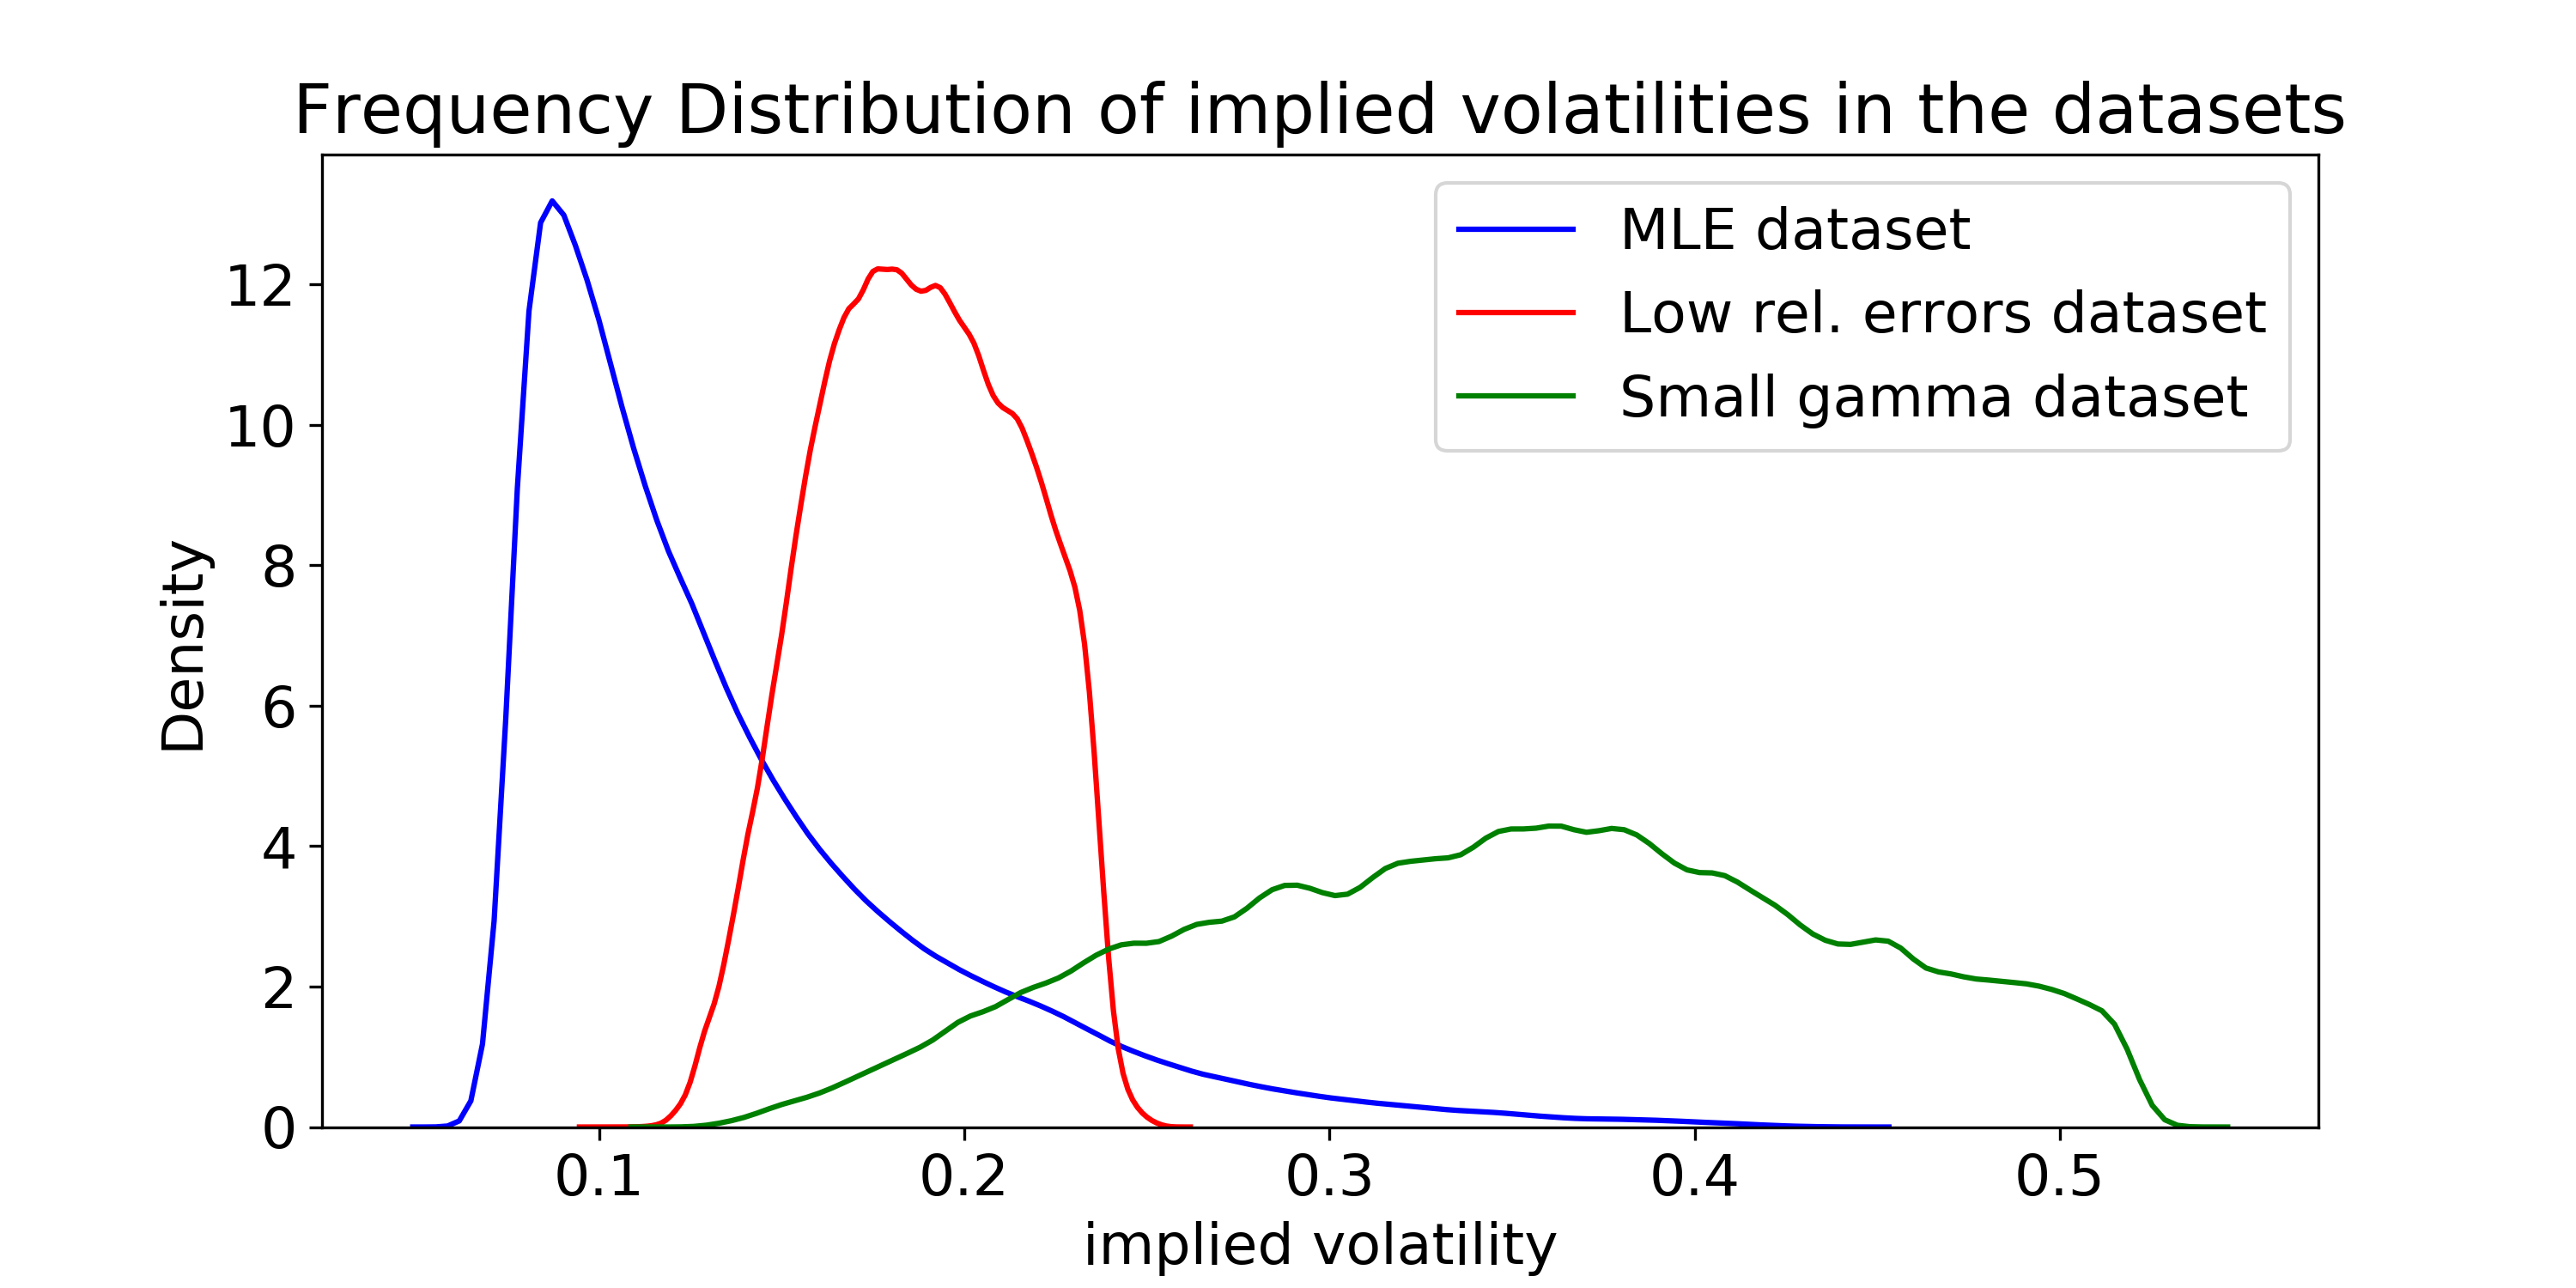
\includegraphics[width=.8\textwidth]{Distribution_Vola_datsets.png}
\caption{Comparison of frequency distributions of implied volatilities of the different datasets}
\label{fig:vol_dist}
\end{figure}
%\fi
%=========================================================================
Figure \ref{fig:vol_dist} visualizes the frequency distribution of the created datasets. The diversity among the dataset is ensured and so each dataset has its justification. 
\subsection{A simple approach on "How to involve real data"}\label{sec:real_data}
Moving from continuous to a discrete model is the first step on providing a setting which can be used in practice. Nevertheless, the major part of this paper covers a model based approach and the usefulness for real application is still unclear. The goal is to find parameter boundaries of $(\omega,\alpha,\beta,\gamma,\lambda)$ for generating a training set, which fits observed S\&P500 data.  Similar to \cite{HestonNandi} and \cite{Book}, we calibrate the HNG model by using Maximum Likelihood estimation. For data points $y_1,\ldots,y_T$, the following optimization problem needs to be solved:
\begin{align}
    \begin{array}{rcll}
  \max\limits_{\omega,\alpha,\beta,\gamma,\lambda}&~&\mathcal{L}\left(y_1,\ldots,y_T|(\omega,\alpha,\beta,\gamma,\lambda)\right)&\\
\mathrm{subject~to}  &~&\alpha\gamma^2+\beta<1\\
  &~&\alpha\geq 0\\
  &~&\beta\geq 0\\
  &~&\omega>0\\
  \end{array} \label{eq:max}
\end{align}
$\mathcal{L}$ is the conditional Log-Likelihood function of the HNG(1,1) model:
\begin{flalign}
\mathcal{L}\left(y_1,\ldots,y_T|(\omega,\alpha,\beta,\gamma,\lambda)\right)=-\dfrac{T}{2}\ln(2\pi)-\dfrac{1}{2}\sum\limits_{t=1}^T \left(\ln(h_t)+ \dfrac{(y_t-r-\lambda h_t)^2}{h_t}  \right)\label{eq:mle}
\end{flalign}
The form \eqref{eq:mle} can be calculated recursively by using identity \eqref{eq:rekursiv}, which is obtained straight from \eqref{eq:HNG}:
\begin{align}
    h_{t+1}= \omega+ \beta h_t +\alpha\dfrac{(Y_t-r-(\lambda+\gamma)h_t)^2}{h_t}\label{eq:rekursiv}
\end{align}\\
A rolling window approach (1000 runs, window length 750 days, starting windows January 2009 - December 2011, ending window January 2013 - December 2015) is used to optimize the parameters. Note that \eqref{eq:max} has some undesirable properties and the success of the optimization is highly dependent on the choice of starting values. We initialise the optimization with the long term expectation $h_0 = \E(h_t)$ as previous literature suggests. Nonetheless, including $h_0$ into the optimization problem does not lead to a significant increase in computational effort and might be subject of further studies.  Table \ref{tab:resultsMLE} and  Figure\ref{fig:paramsMLE} summarize the results. 
\begin{table}[!ht]
\centering
\begin{tabular}{|c|r|r|r|r|r|}
\hline
 & \multicolumn{1}{c|}{$\omega$} & \multicolumn{1}{c|}{$\alpha$} & \multicolumn{1}{c|}{$\beta$} & \multicolumn{1}{c|}{$\gamma$} & \multicolumn{1}{c|}{$\lambda$} \\ \hline
Average & 2.894e-6 & 1.235e-6 & 0.661 & 473.243 & 10.384 \\ \hline
Standard Deviation & 1.006e-6 & 2.649e-7 & 0.087 & 11.489 & 2.871e-5 \\ \hline
5\% Quantile & 1.587e-6 & 9.903e-7 & 0.527 & 456.564 & 5.052 \\ \hline
95\% Quantile & 5.526e-6 & 1.610e-6 & 0.741 & 489.853 & 14.214 \\\hline
\end{tabular}\label{tab:resultsMLE}\vspace{0.1cm}
\caption{Rolling estimation of Heston and Nandi between 2012 and 2015 on S\&P500}
\end{table}
\begin{figure}[!ht]
    \centering
    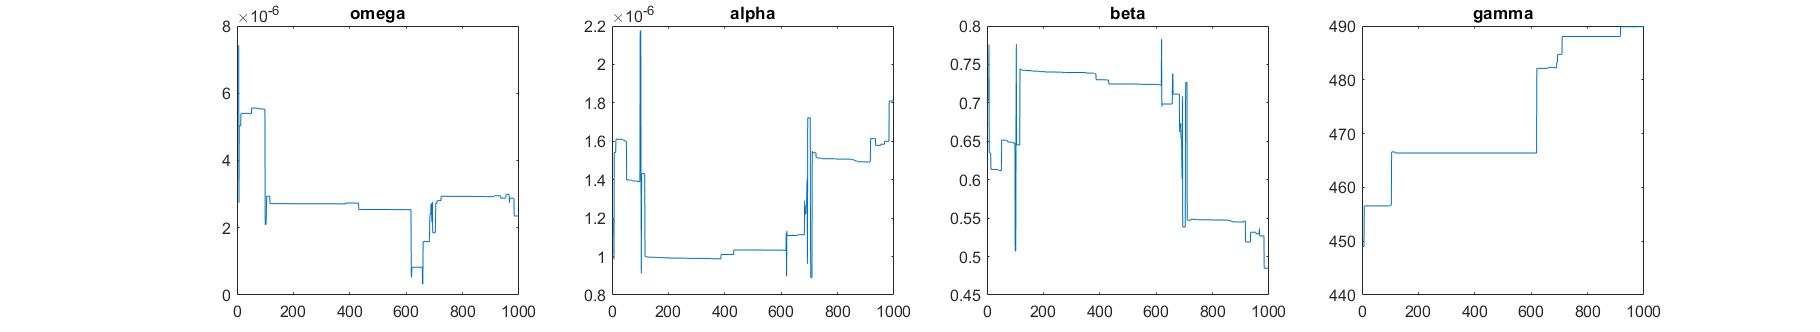
\includegraphics[width=\linewidth]{parameter_mle.png}
    \caption{Rolling estimation of Heston and Nandi between 2012 and 2015 on S\&P500}
    \label{fig:paramsMLE}
\end{figure}\\
The  symmetric 90\% confidence interval of these parameters is included in one parameter set, which is used to train the neural net (cf. Section \ref{sec:setupmle}). This procedure should assure that the neural net is capable of pricing calls on S\&P500 traded in the corresponding years.\\
Besides the model fit of this parameter setup (cf. Section \ref{sec:price_surf}), we want to analyse how well this rudimentary approach fits real option prices. To test this, prices of European style call options with underlying S\&P500 traded between January 2010 and December 2015 are used. Options with a open interest or a trading volume of less then 100 were excluded. Additionally options with a maturity of more then 1 year and less then 30 days were excluded. The dataset contains 73.918 call options. The observed Moneyness is 0.6 between 2.8. Due to the small amount of option with extreme high/low Strikes, we only consider options with relative Strike $\frac{K}{S_0}$ between 0.9 and 1.1. Prices of options with same characteristics are averaged out to get a unique price. These differences may occur from market microstructure effects, semiefficient markets or a change in interest rate. Per year a single price surface is generated and cubic interpolation is used to smooth the surface and fit missing values. Figure \ref{fig:real_surf} shows the fitted surface and real options prices in 2015. These surfaces are now used to calibrate the trained net. The results can be found in Section \ref{sec:results_sp500}.
%=====================================
%\iffalse
%\begin{wrapfigure}{c}{0.7\textwidth}[!ht]
\begin{figure}[!ht]
   \centering
  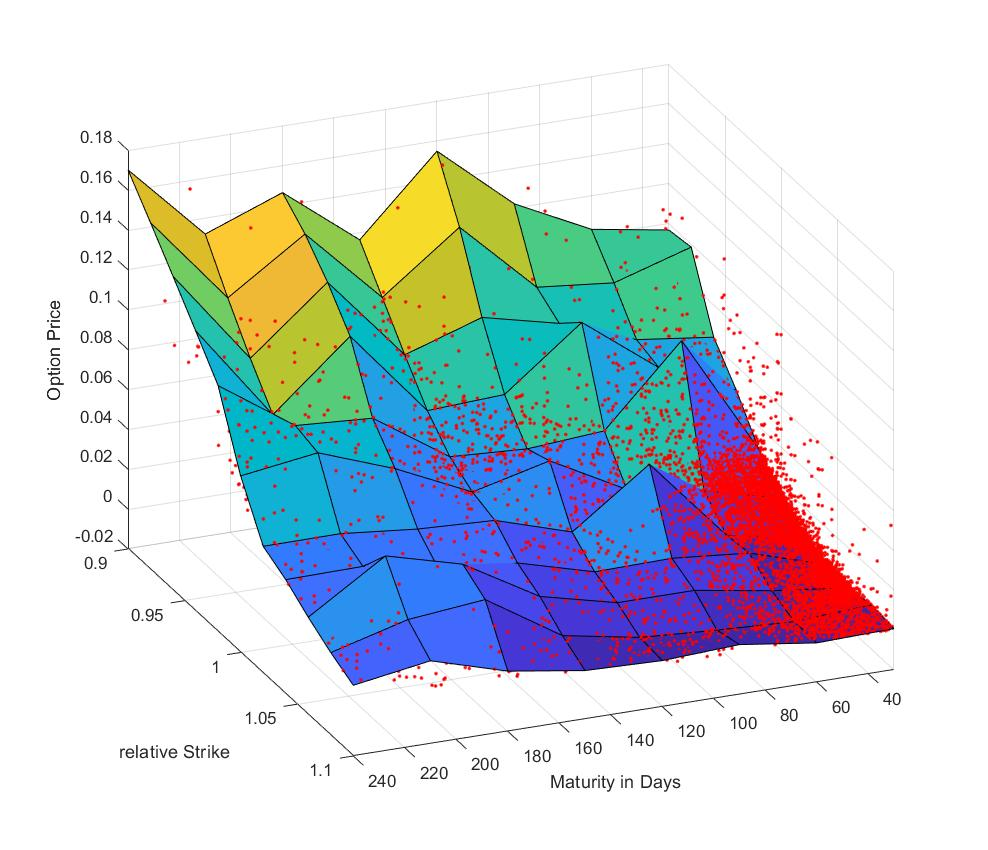
\includegraphics[width=0.5\textwidth]{calls_surface_sp500_2015.jpg}
   \caption{Call prices of 2015 and fitted price surface}
    \label{fig:real_surf}
\end{figure}
%\end{wrapfigure}
%\fi
%=======================
\section{Results}
\subsection{Volatility surfaces}\label{sec:vola_results}
As a starting point we analyse the results of the dataset based on the $90\%$ Maximum Likelihood confidence interval. Figure \ref{fig:MLE_NN_rel_err} shows that the vast majority of average relative testing errors of the neural network is located significantly below $0.7\%$ on the strike-maturity grid. Nevertheless the maximum relative errors rise up to $40\%$ in the corners where the extreme scenarios lie (small maturity combined with high or low strikes). All in all the approximation results of the neural network are in the same order of magnitude as the findings of Horvath et al. \cite{Blanka} regarding the Bergomi model. \newline
Figure \ref{fig:MLE_par_sen} and \ref{fig:MLE_smile} indicate that the Maximum Likelihood based dataset probably is not the best dataset to use for training the neural network. The generated scenarios are incapable to reproduce a volatility smile or a more complex volatility surface which would be more challenging for the neural network to approximate. Additionally we observe that the calibrated parameters, especially $\alpha, \gamma^*$ and $\omega$, differ up to $9\%$ on average from the true parameters in the test set. \newline
As the dataset based on Maximum Likelihood estimation doesn't fully satisfy our high demands we generate two additional datasets.
\newline 
%=========================================================================
%Figure 1 MLE NN relative errors
%\iffalse %zum Auskommentieren
\begin{figure}[!ht]
\centering
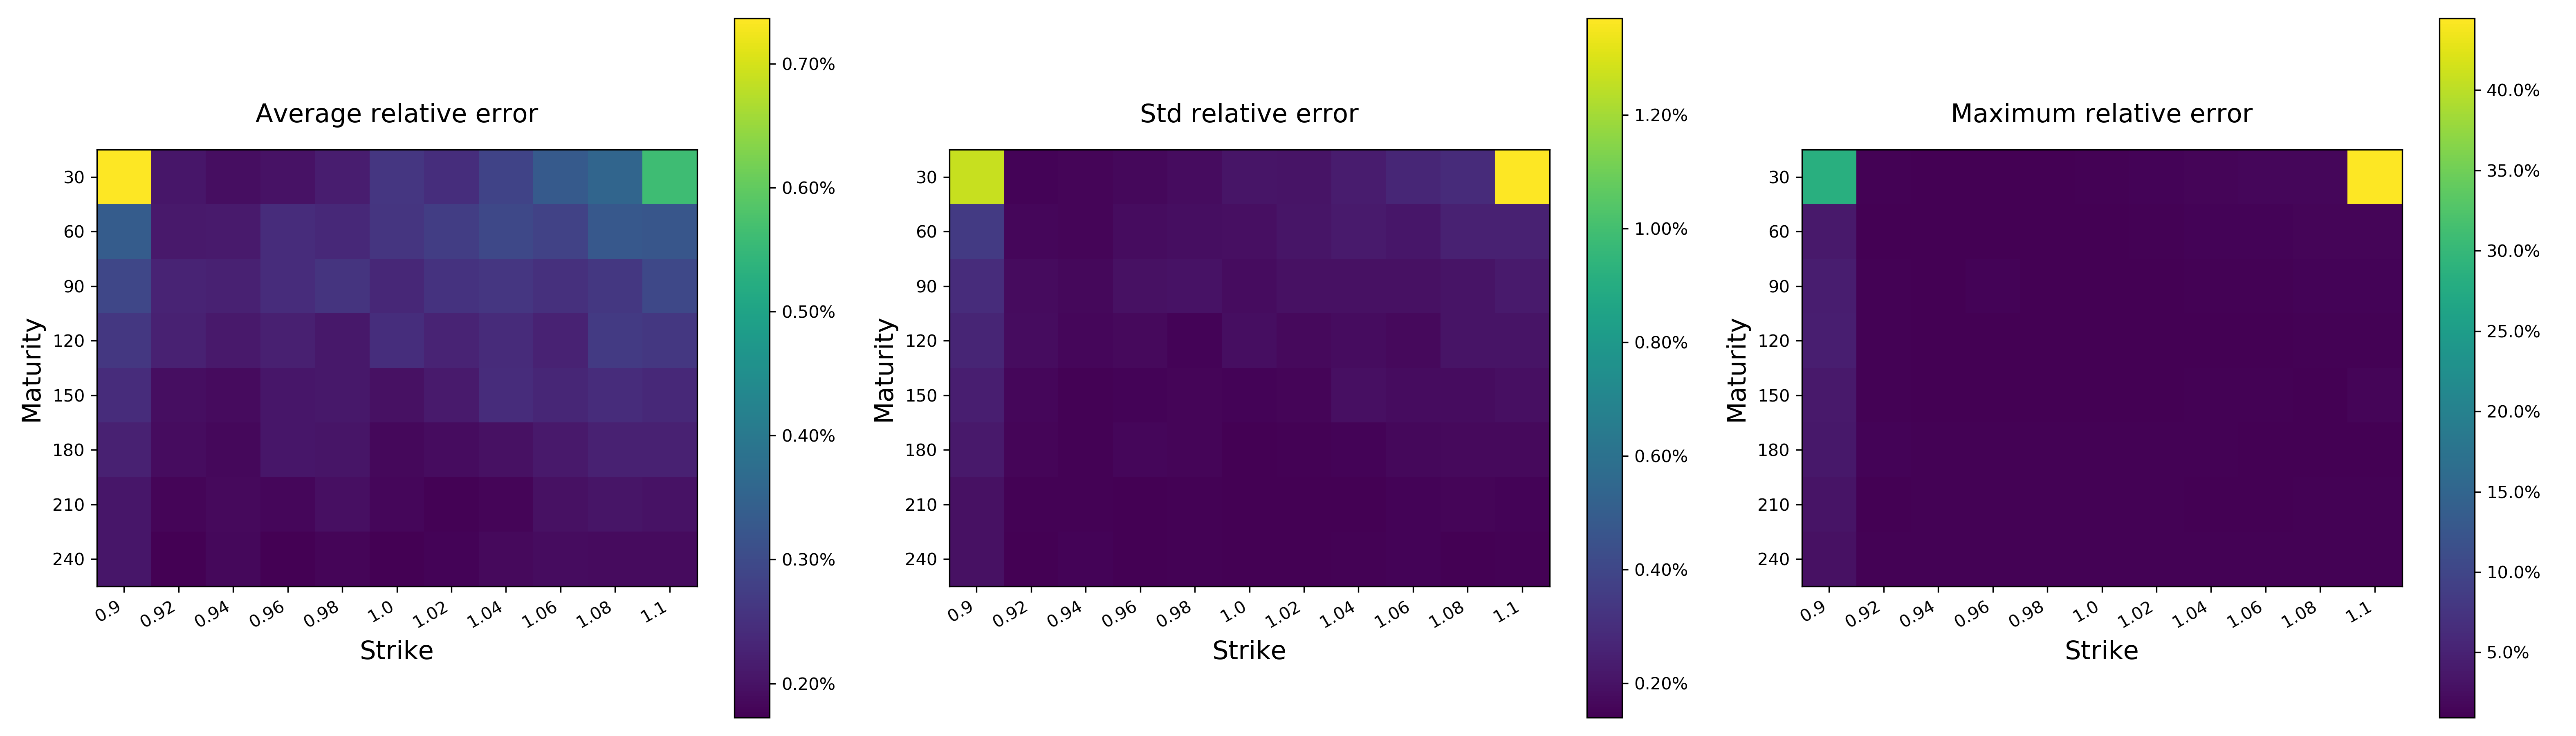
\includegraphics[width=\textwidth]{MLE_Vola_HNG_NNErrors.png}
\caption{$90\%$ Maximum Likelihood confidence interval - Relative errors of the neural network predicted volatilities compared to true volatilities in the test set}
\label{fig:MLE_NN_rel_err}
\end{figure}
%=========================================================================
%Figure 2 MLE NN Parameter sensitivities
\begin{figure}[!ht]
\centering
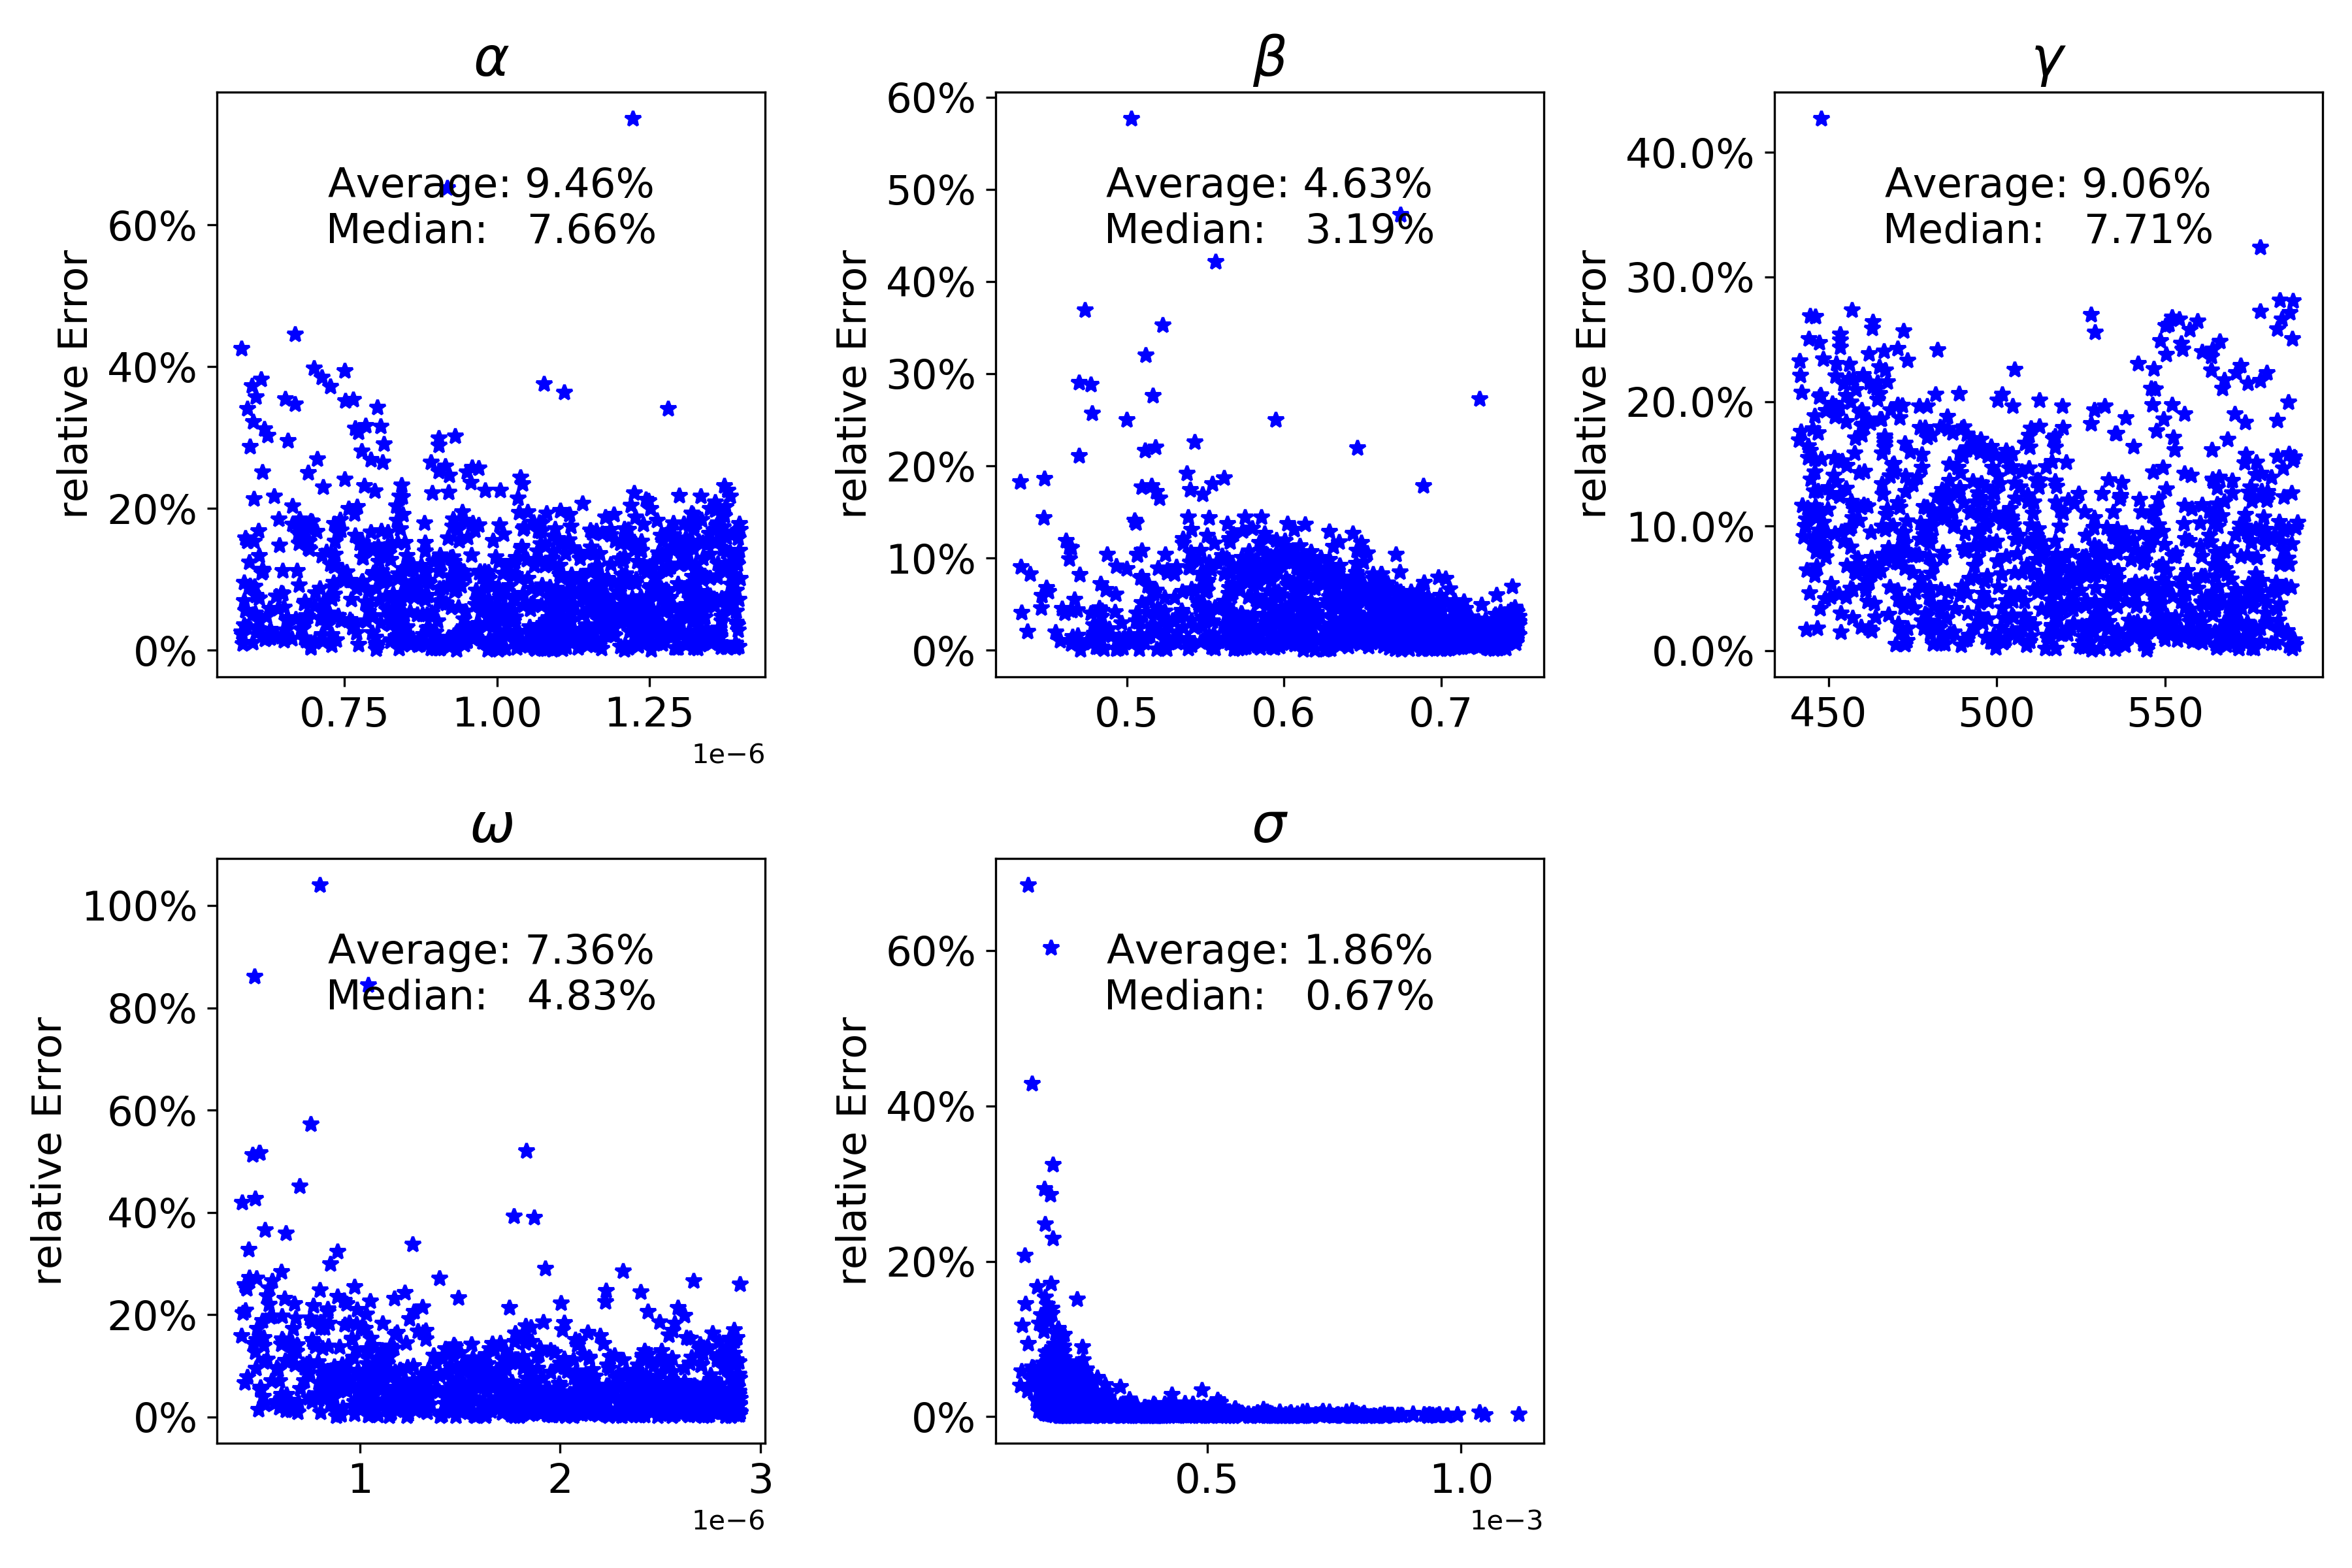
\includegraphics[width=\textwidth]{MLE_Vola_HNG_ParameterRelativeErrors.png}
\caption{$90\%$ Maximum Likelihood confidence interval - Relative errors of the parameters after calibration with Levenberg-Marquardt compared to true parameters in the test set}
\label{fig:MLE_par_sen}
\end{figure}
%=========================================================================
%Figure 3 MLE smile
\begin{figure}[!ht]
\centering
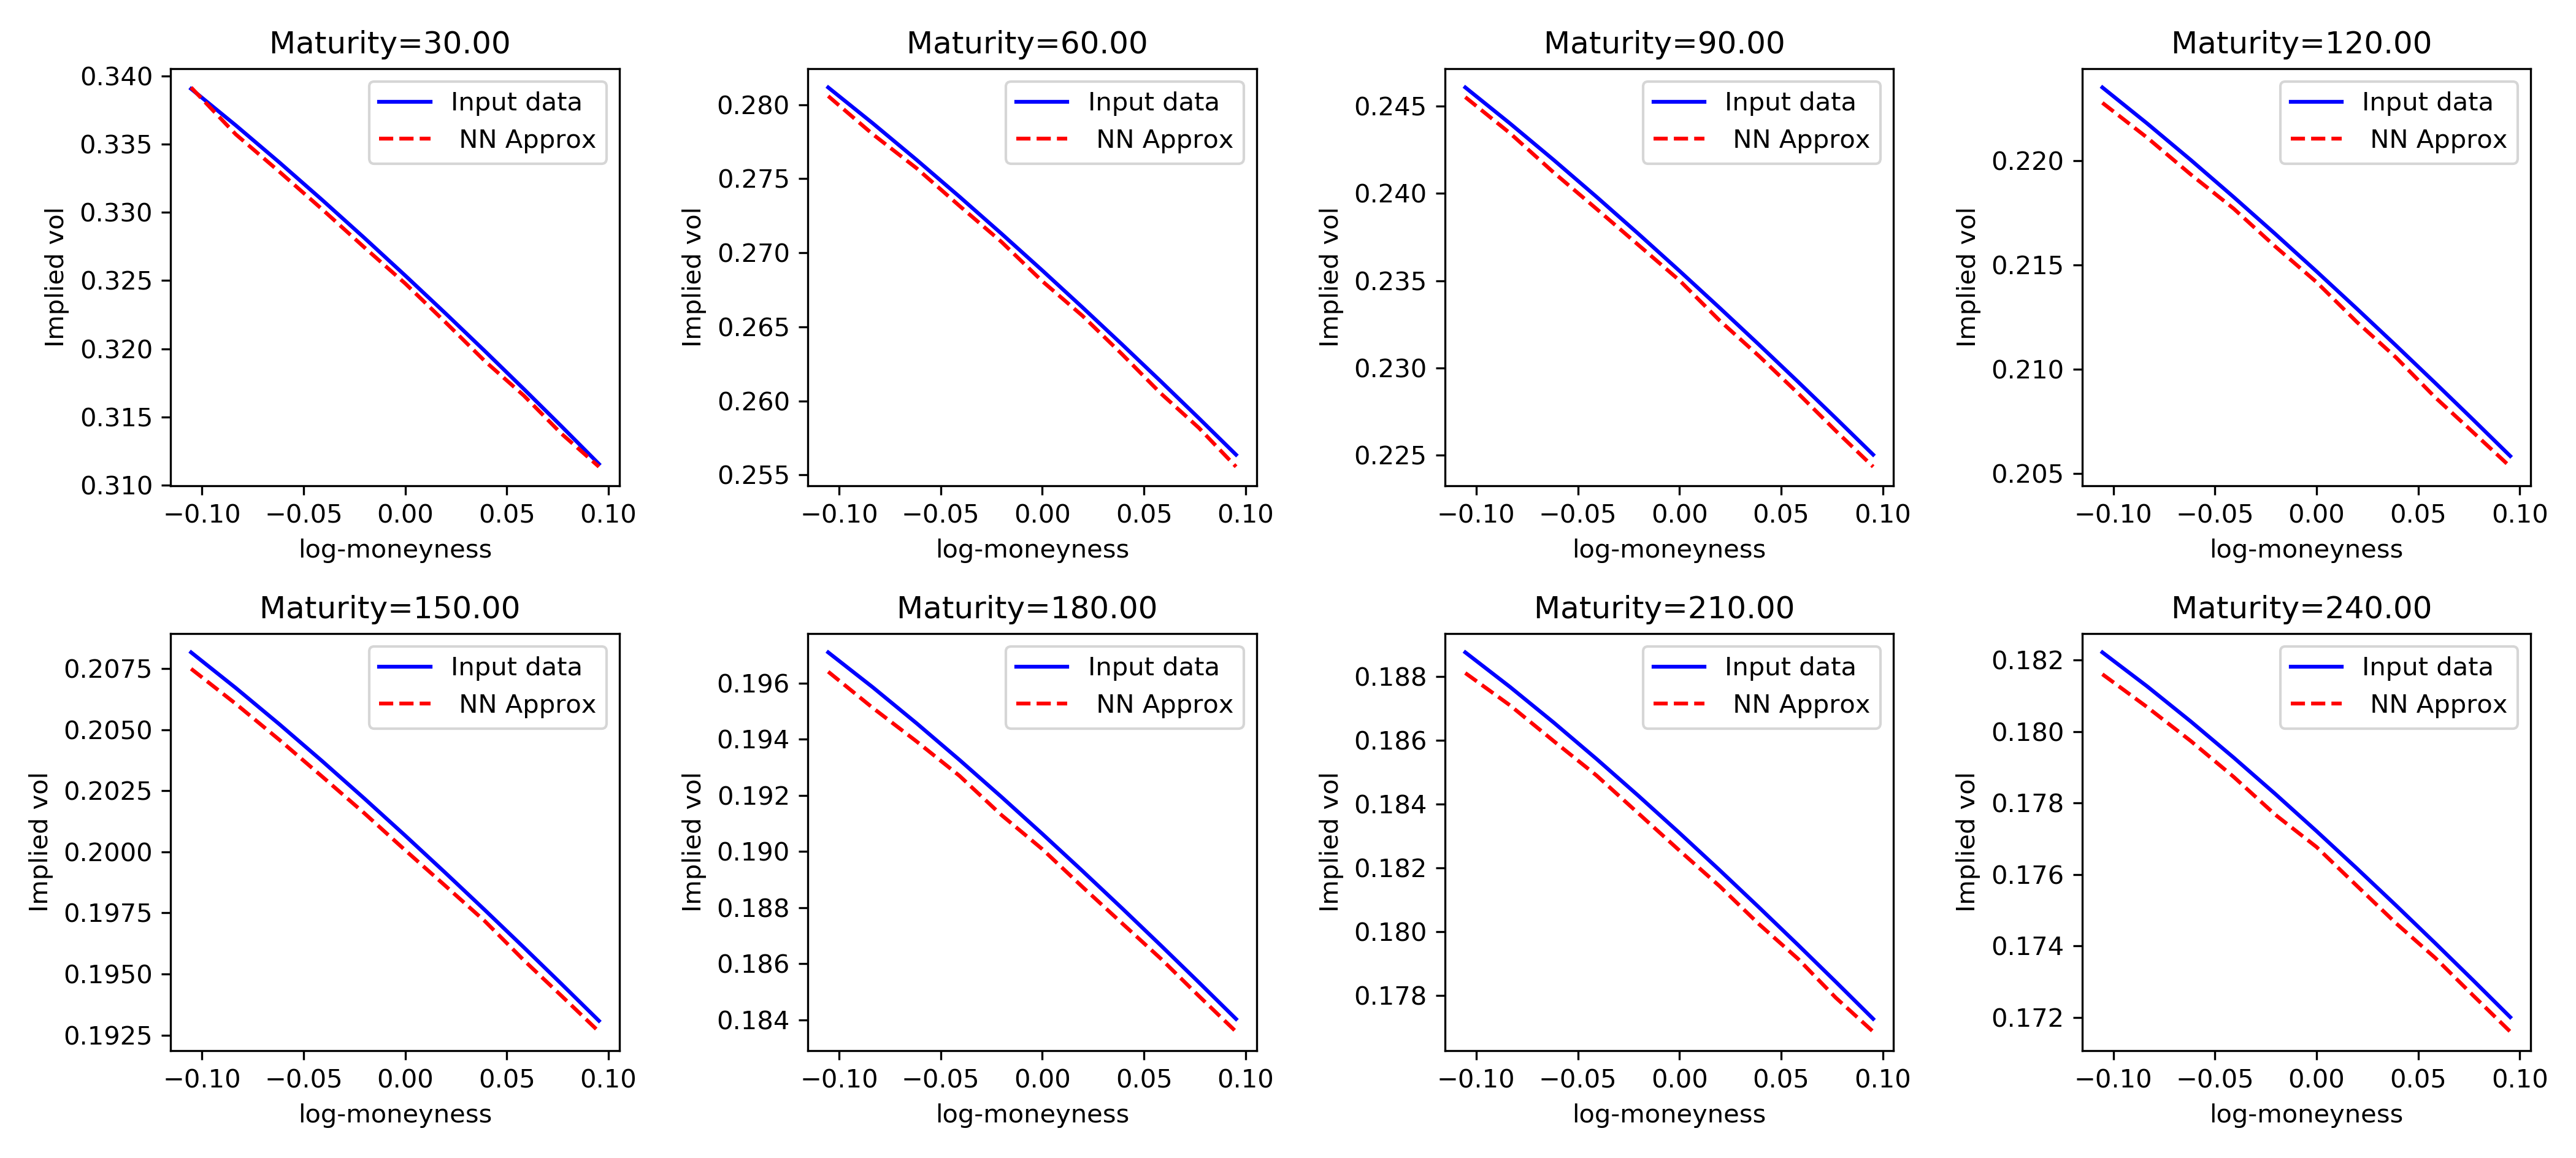
\includegraphics[width=\textwidth]{MLE_Vola_HNG_smile.png}
\caption{$90\%$ Maximum Likelihood confidence interval - Comparison of neural network predicted volatilites and true volatilites in the test set}
\label{fig:MLE_smile}
\end{figure}
%\fi %zum Auskommentieren
%=========================================================================
First, we create a dataset which has the objective of minimize the neural network approximation error of the implied volatility surface. This task is very time consuming since the intervals are subject to constraints (cf. equations \ref{eq:max}) and the neural network needs to get along with the generated dataset, too. Additionally, we observe that the shape of the implied volatility surface is very sensitive to only small changes in parameter values. Finally, we come up with a fully viable dataset which leads to mean relative errors of $0.06\%$ and smaller and maximum relative errors of $2.3\%$ and smaller (cf. Figure \ref{fig:low_err_NN_rel_err}). Figure \ref{fig:low_err_smile} visualizes that the volatilities in this set of scenarios follow a more concave process along moneyness.
%=========================================================================
%Figure 4 low errors NN relative errors
%\iffalse %zum Auskommentieren
\begin{figure}[!ht]
\centering
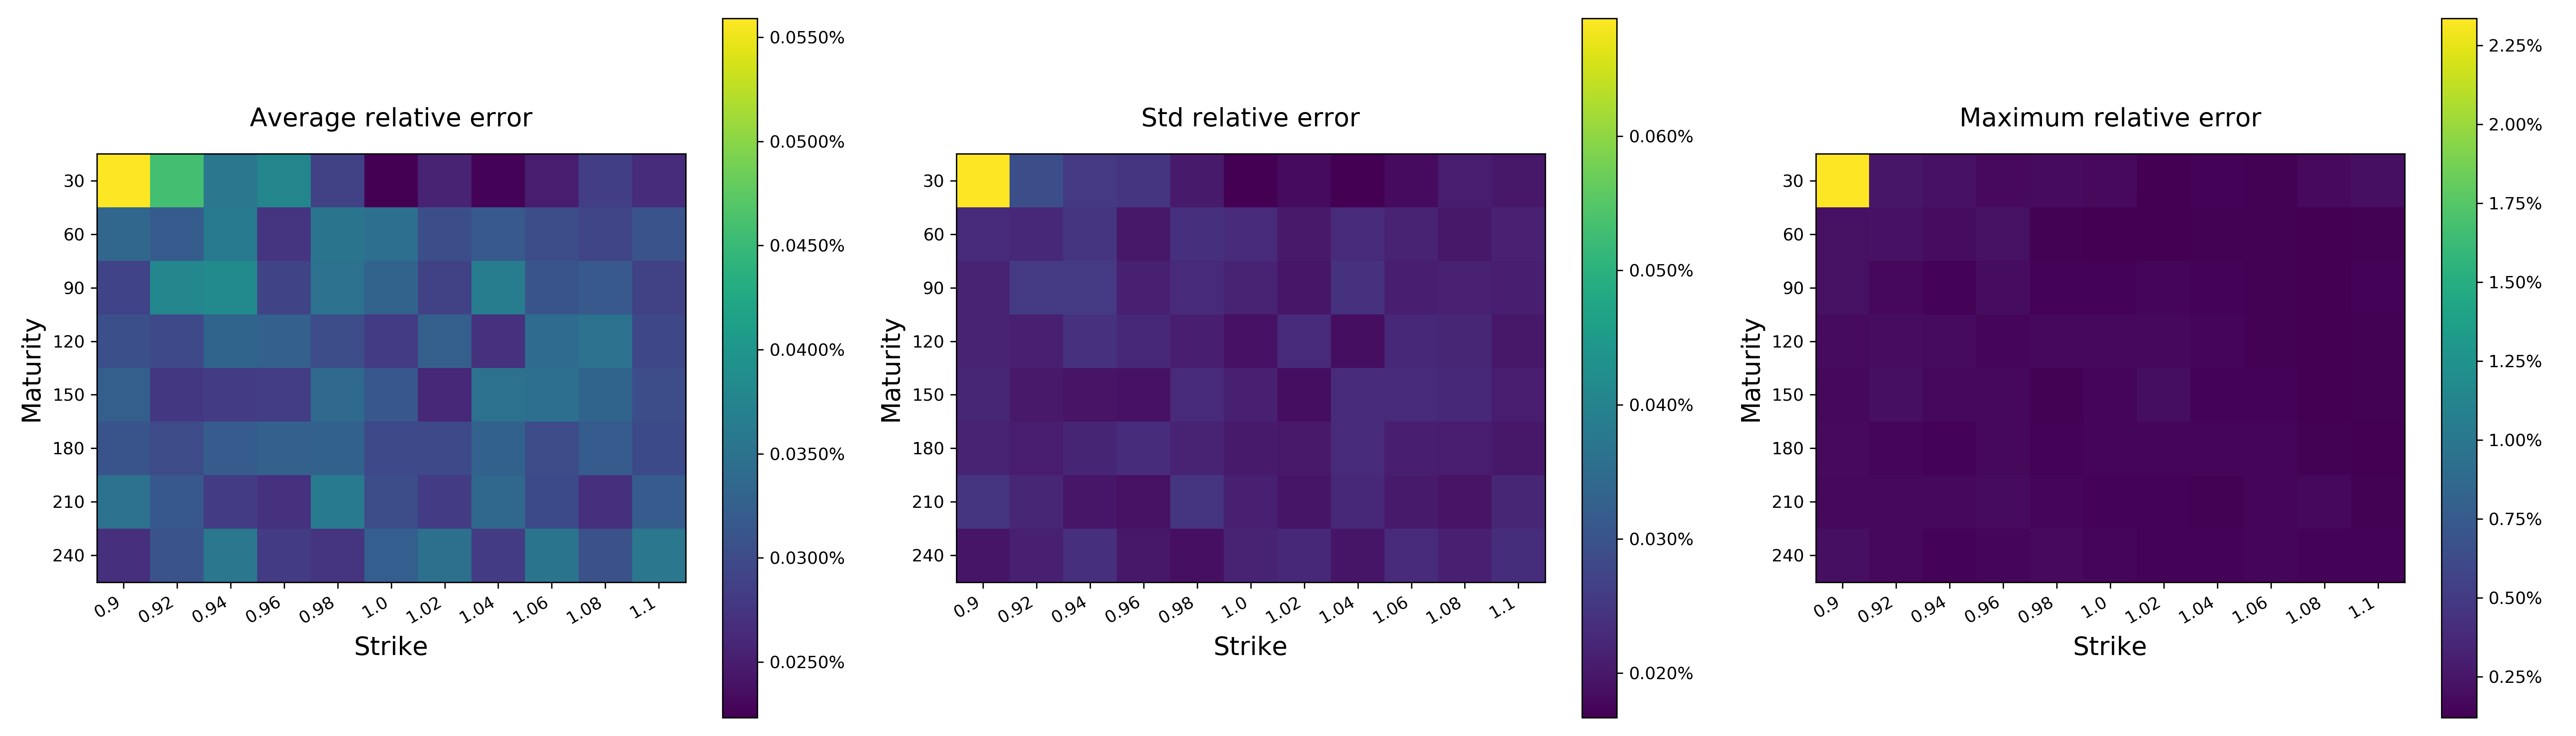
\includegraphics[width=\textwidth]{Low_error_Vola_HNG_NNErrors.png}
\caption{Best fit - Relative errors of the neural network predicted volatilities compared to true volatilities in the test set}
\label{fig:low_err_NN_rel_err}
\end{figure}
%=========================================================================
%Figure 5 low errors smile
\begin{figure}[!ht]
\centering
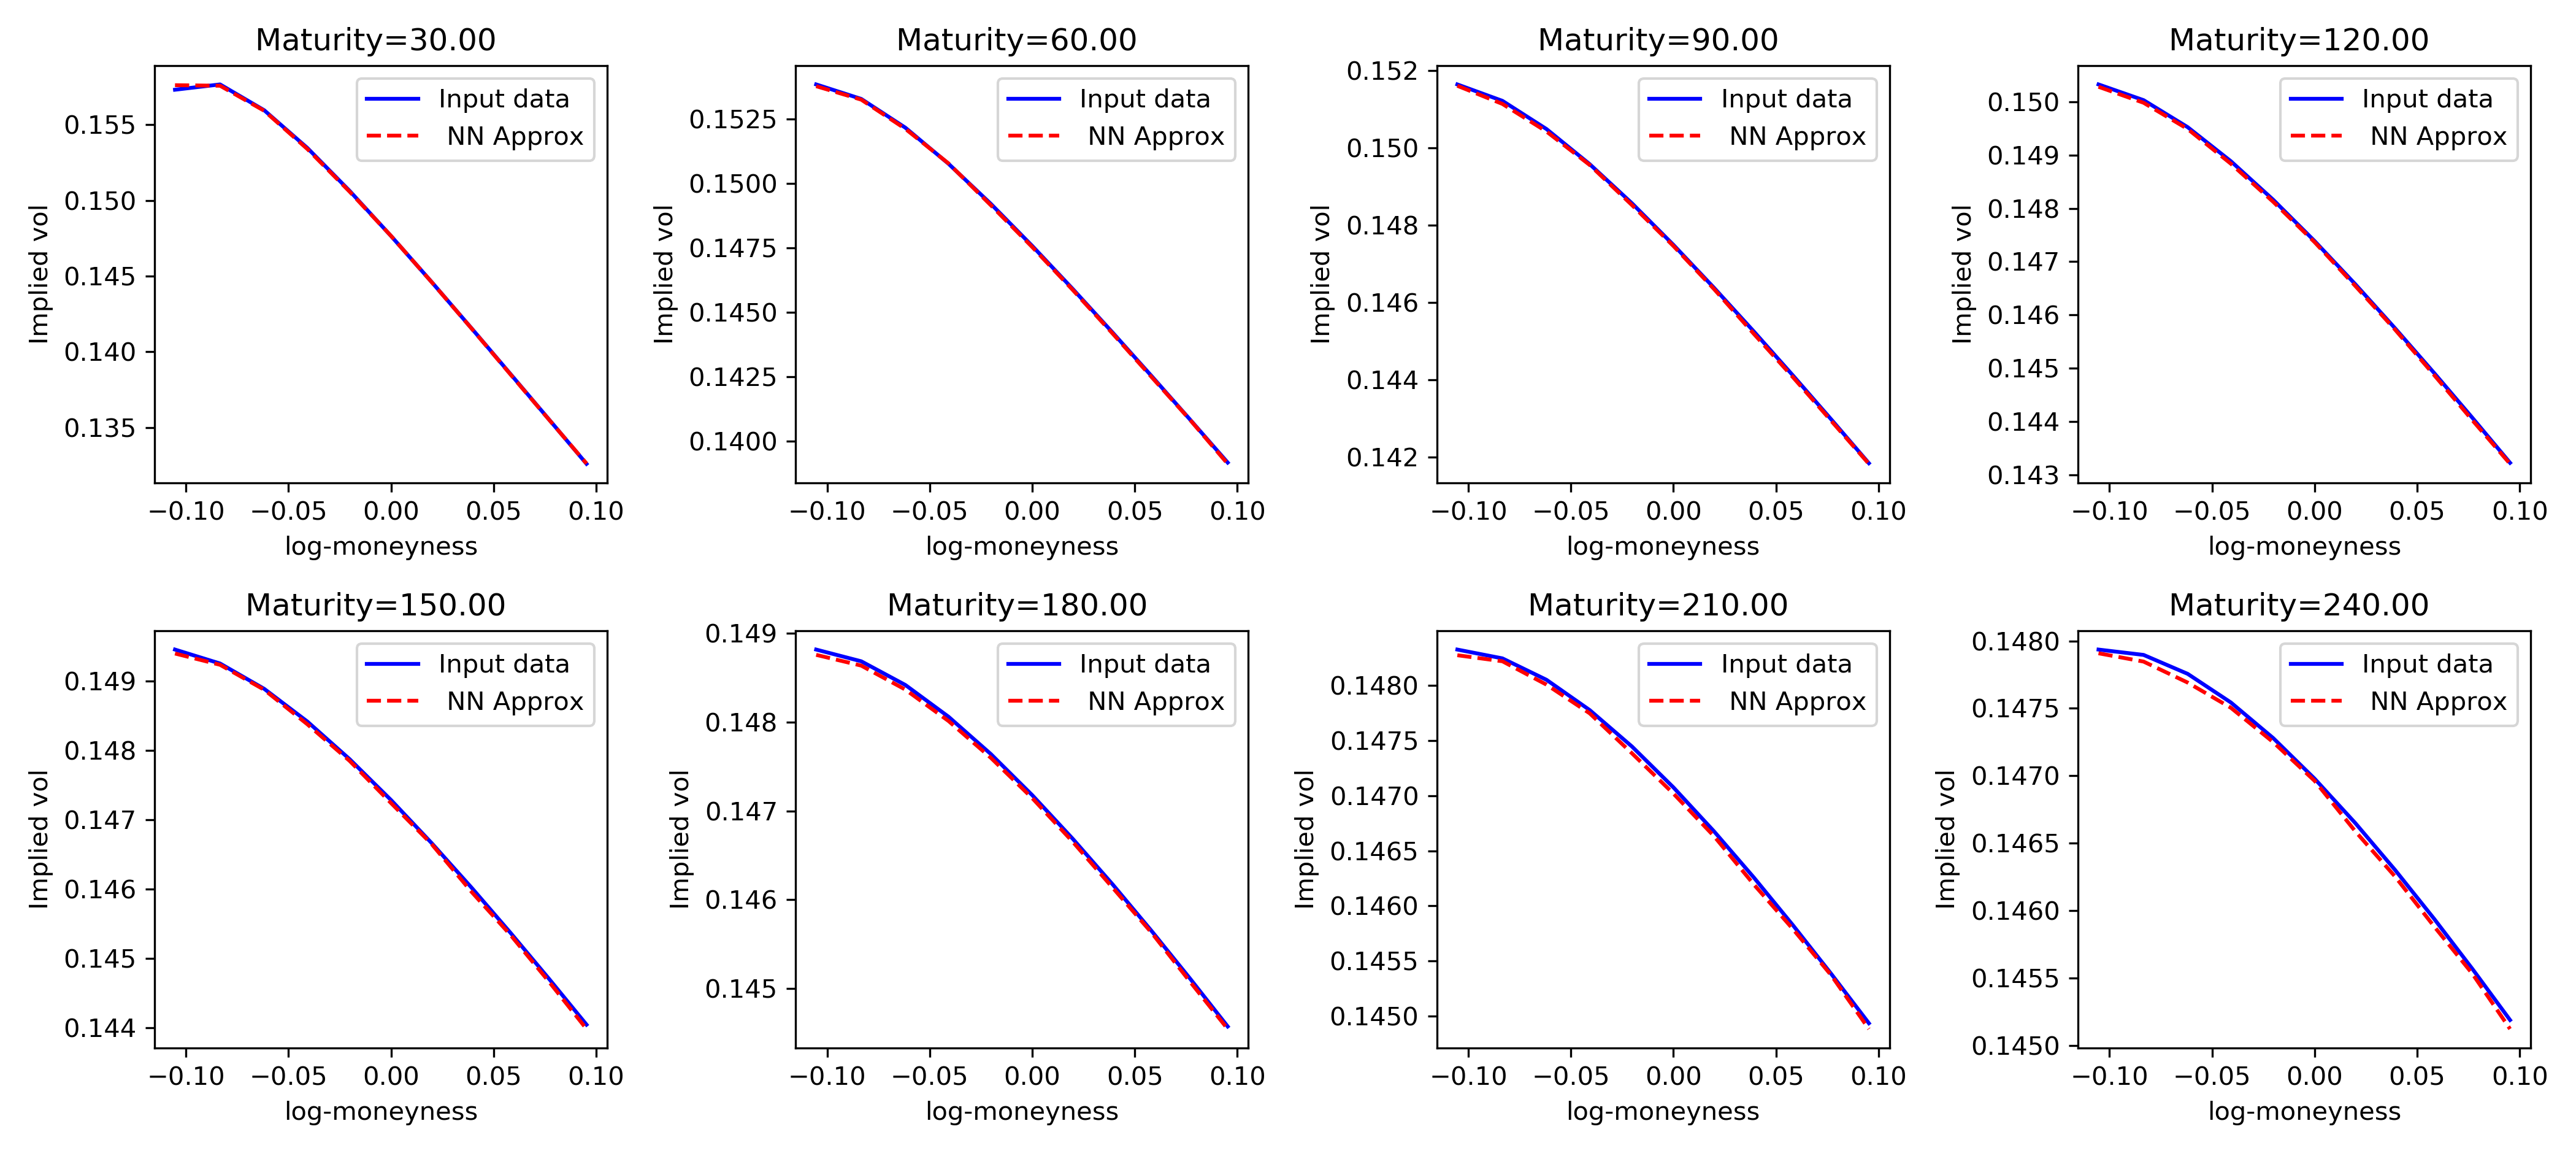
\includegraphics[width=\textwidth]{Low_error_Vola_HNG_smile.png}
\caption{Best fit - Comparison of neural network predicted volatilites and true volatilites in the test set}
\label{fig:low_err_smile}
\end{figure}

%=========================================================================
%Figure 6 low errors NN Parameter sensitivities
\begin{figure}[!ht]
\centering
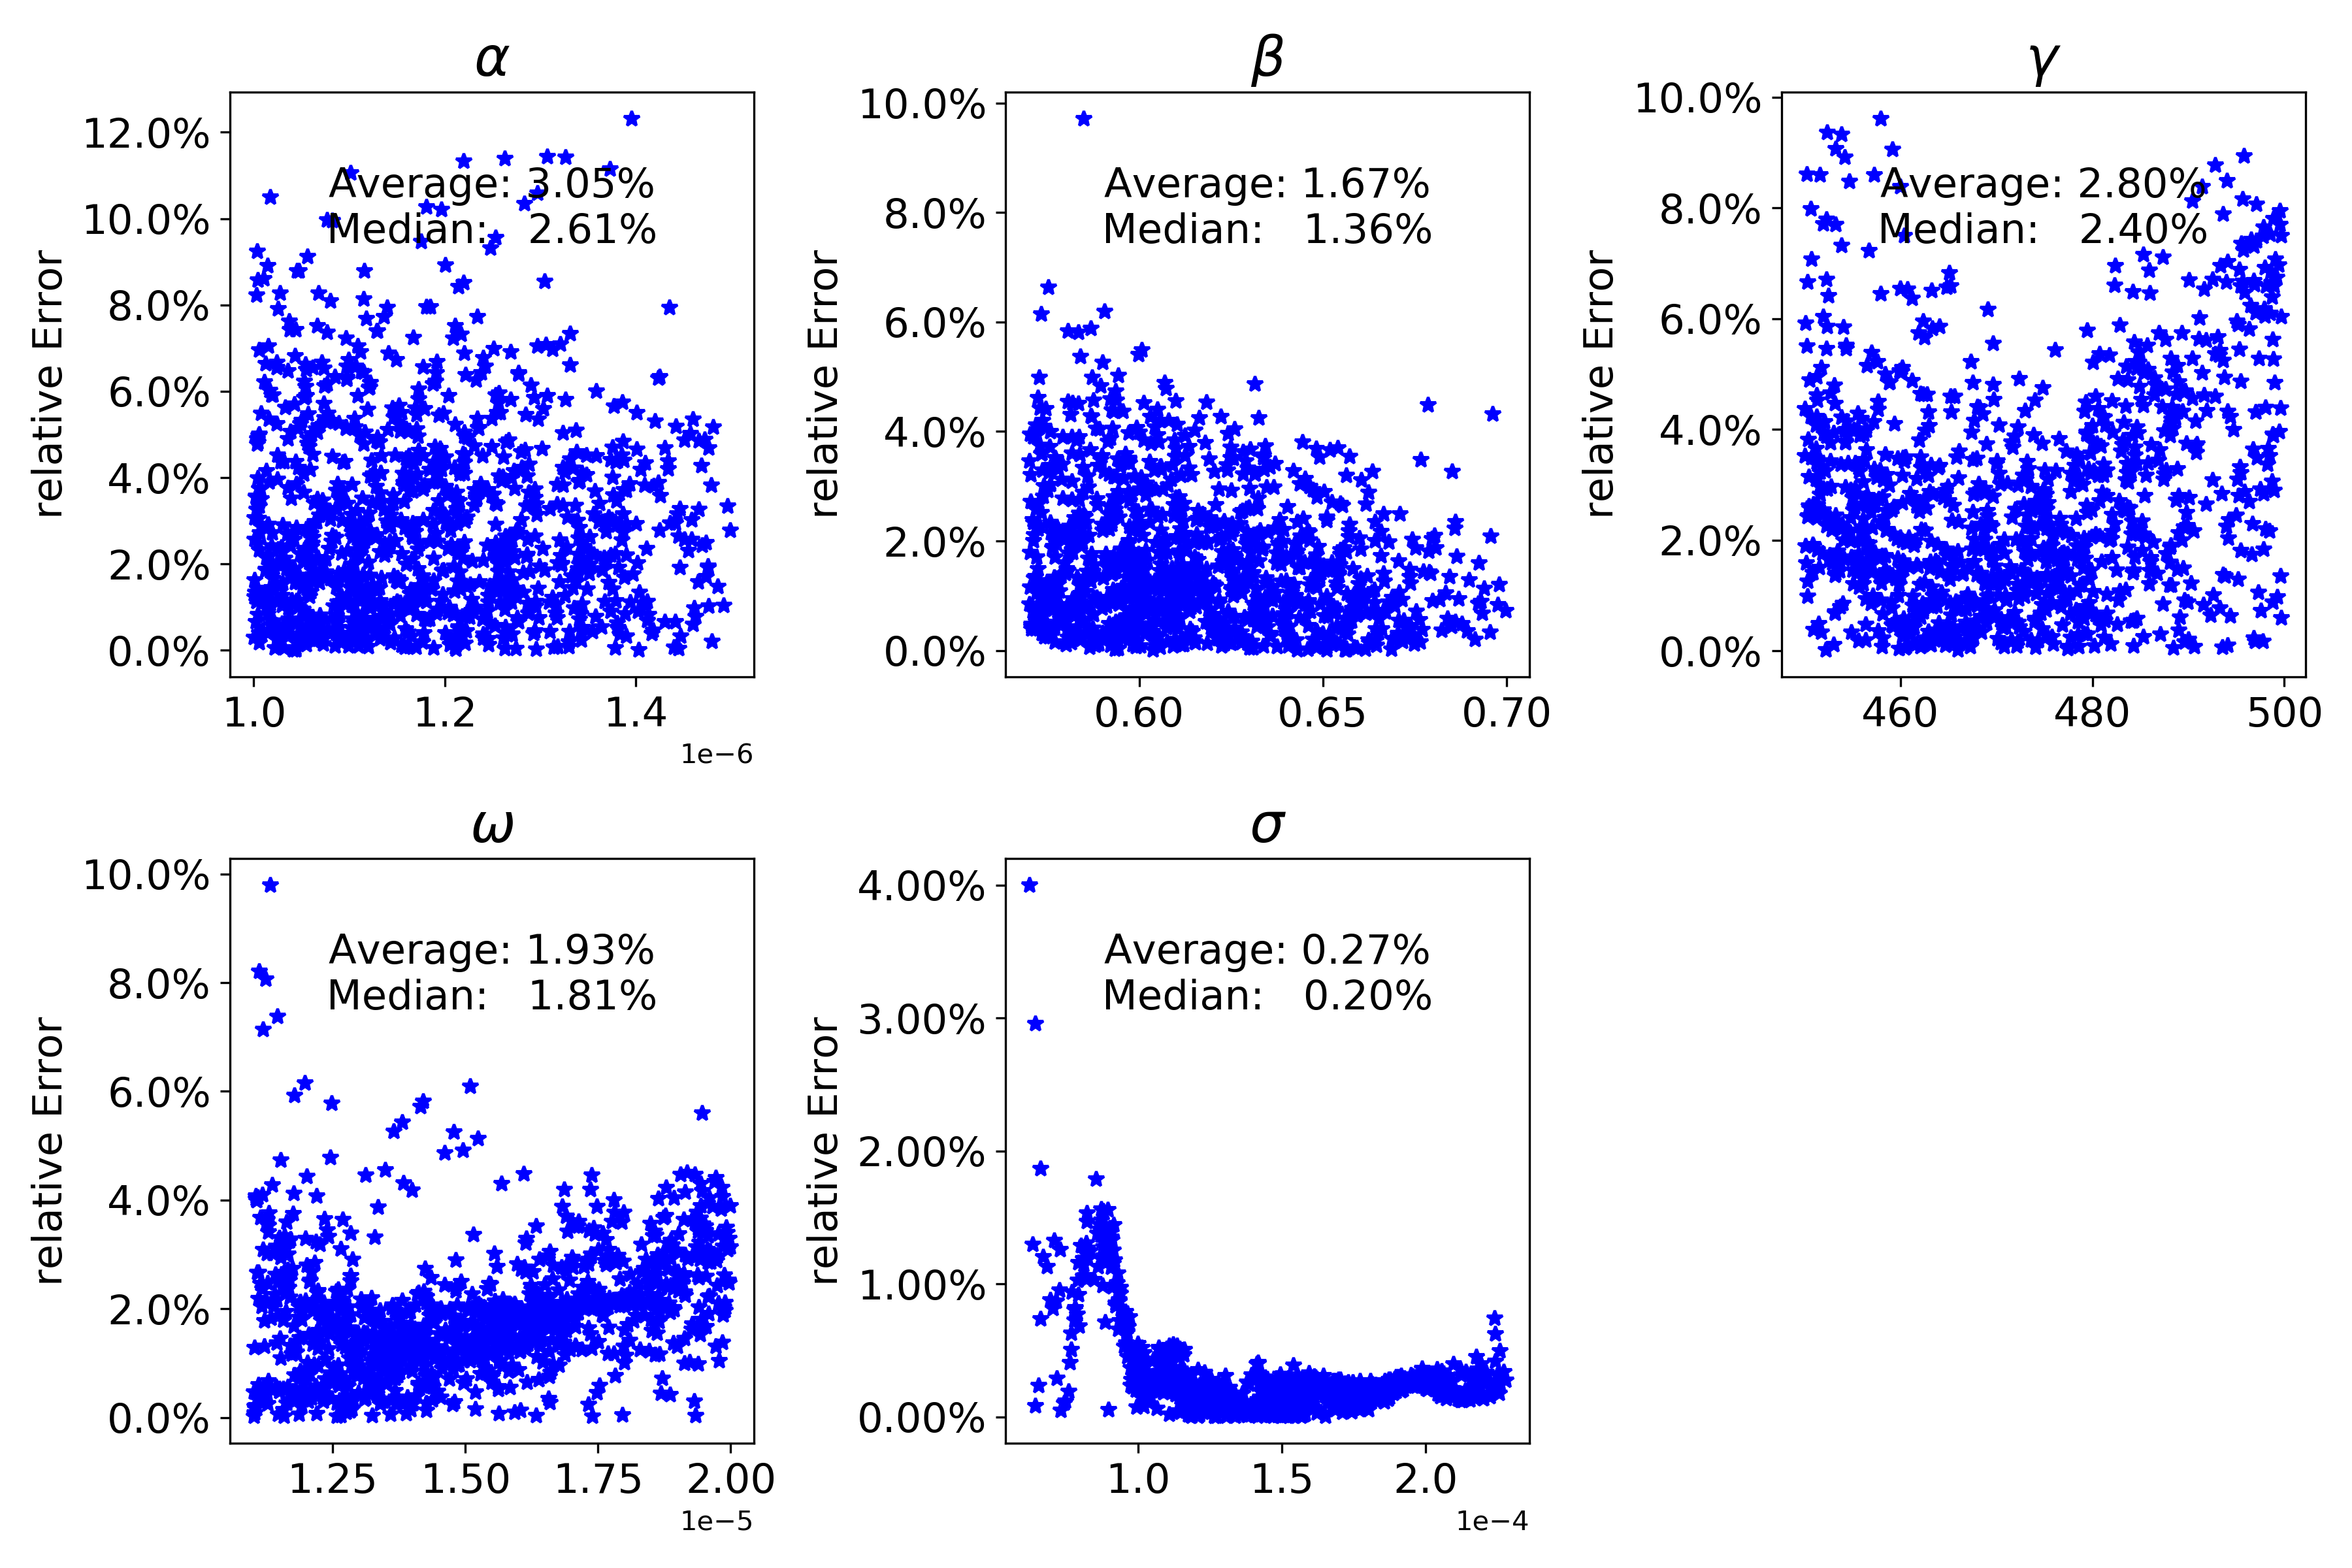
\includegraphics[width=\textwidth]{Low_error_Vola_HNG_ParameterRelativeErrors.png}
\caption{Best fit - Relative errors of the parameters after calibration with Levenberg-Marquardt compared to true parameters in the test set}
\label{fig:low_err_par_sen}
\end{figure}
%\fi %zum Auskommentieren
%=========================================================================
%\newline
The second alternative dataset contains implied volatility surfaces with a pronounced smile. This is achieved by using $\gamma^*$ parameters close to zero. Figure \ref{fig:Small_g_NN_rel_err} demonstrates that the network is able to replicate the modified shape of surface: The mean relative error is predominantly smaller than $0.1\%$, the maximum relative error smaller than $8\%$. Also Figure \ref{fig:Small_g_smile} and \ref{fig:Small_g_vola_surface} illustrate the quite accurate predicted smile in particular for short maturities. It should be mentioned that the whole volatility surface is still quite flat, e.g. in Figure \ref{fig:Small_g_vola_surface} the volatilities range from $27.2\%$ to $28\%$. We tried a lot to install parameter boundaries which yield greater differences in volatility height, but we don't manage to find them so far. \newline
In Figure \ref{fig:Small_g_par_sen} the optimized $\omega$ parameter has a mean relative error of $19\%$, which is the largest among all parameters. \newline
The plots shown in this paragraph are inspired by Horvath et al. \cite{Blanka}. This visualized form of well structured summaries also helps to compare our results with the result they present in their paper. To keep this section transparent we don't include all plots. For instance RMSE plots are listed in Appendix \ref{sec:app_vola_plots}.
%=========================================================================
%Figure 7 Small g NN relative errors
%\iffalse %zum Auskommentieren
\begin{figure}[!ht]
\centering
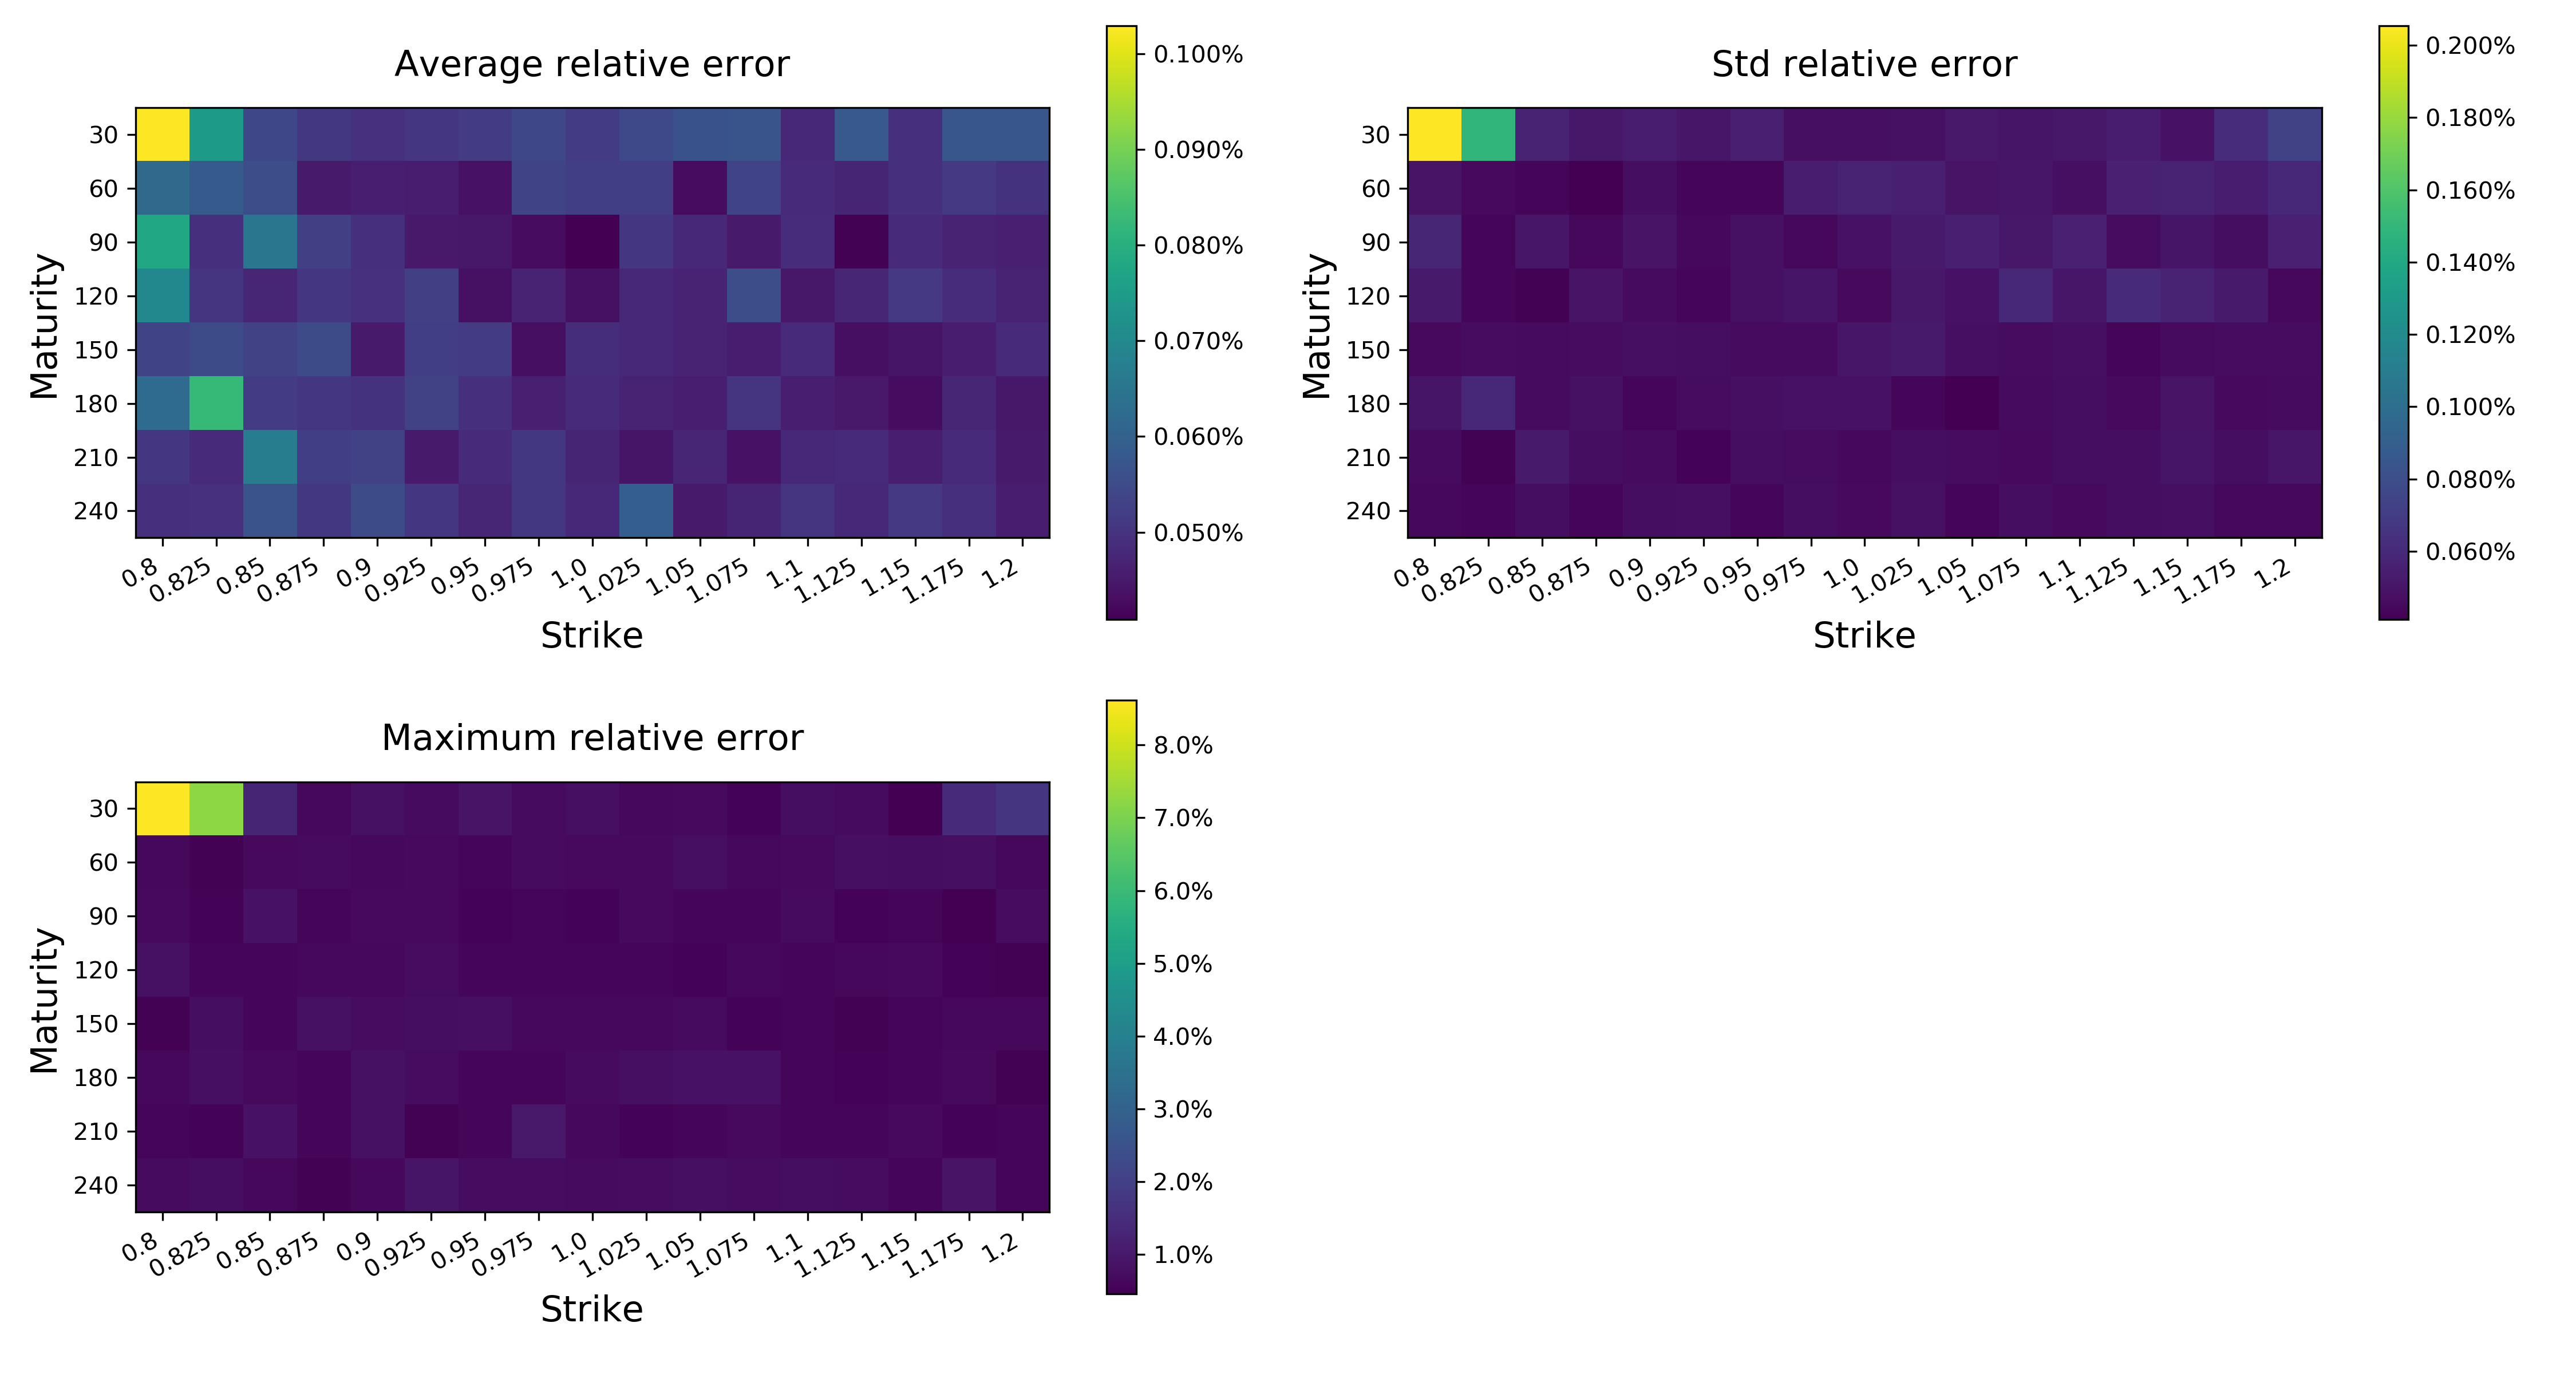
\includegraphics[width=\textwidth]{Small_g_Vola_HNG_NNErrors.png}
\caption{Small $\gamma^*$ - Relative errors of the neural network predicted volatilities compared to true volatilities in the test set}
\label{fig:Small_g_NN_rel_err}
\end{figure}
%=========================================================================
%Figure 8 Small g smile
\begin{figure}[!ht]
\centering
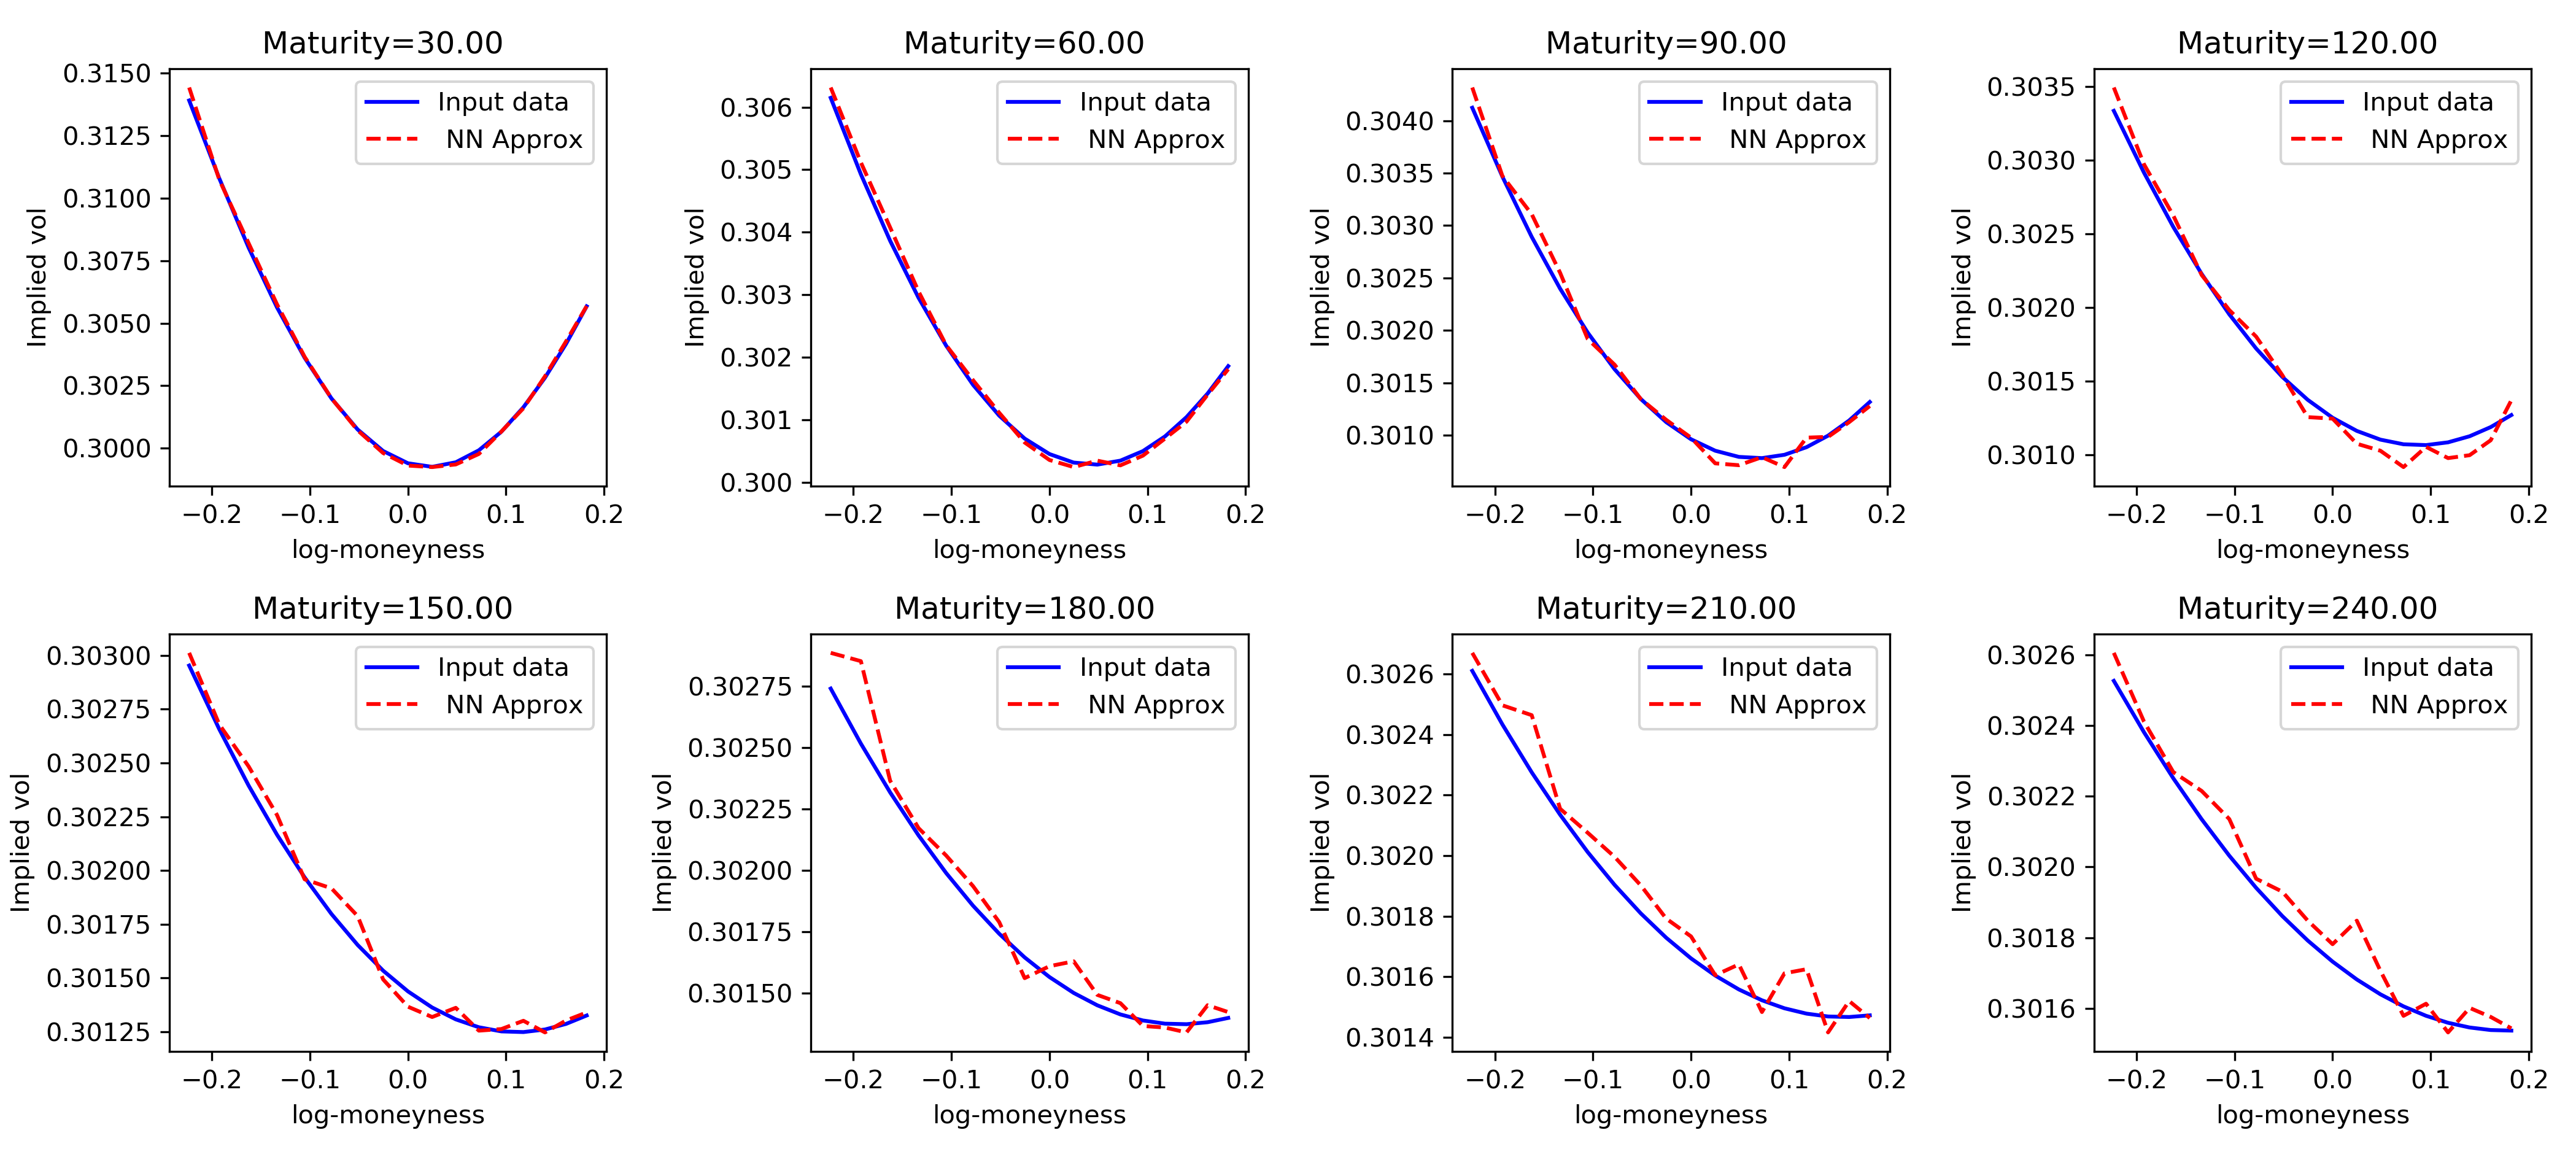
\includegraphics[width=\textwidth]{Small_g_Vola_HNG_smile.png}
\caption{Small $\gamma^*$ - comparison of neural network predicted volatilites and true volatilites in the test set}
\label{fig:Small_g_smile}
\end{figure}
%=========================================================================
%Figure 9 Small g volatility surface
\begin{figure}[!ht]
\centering
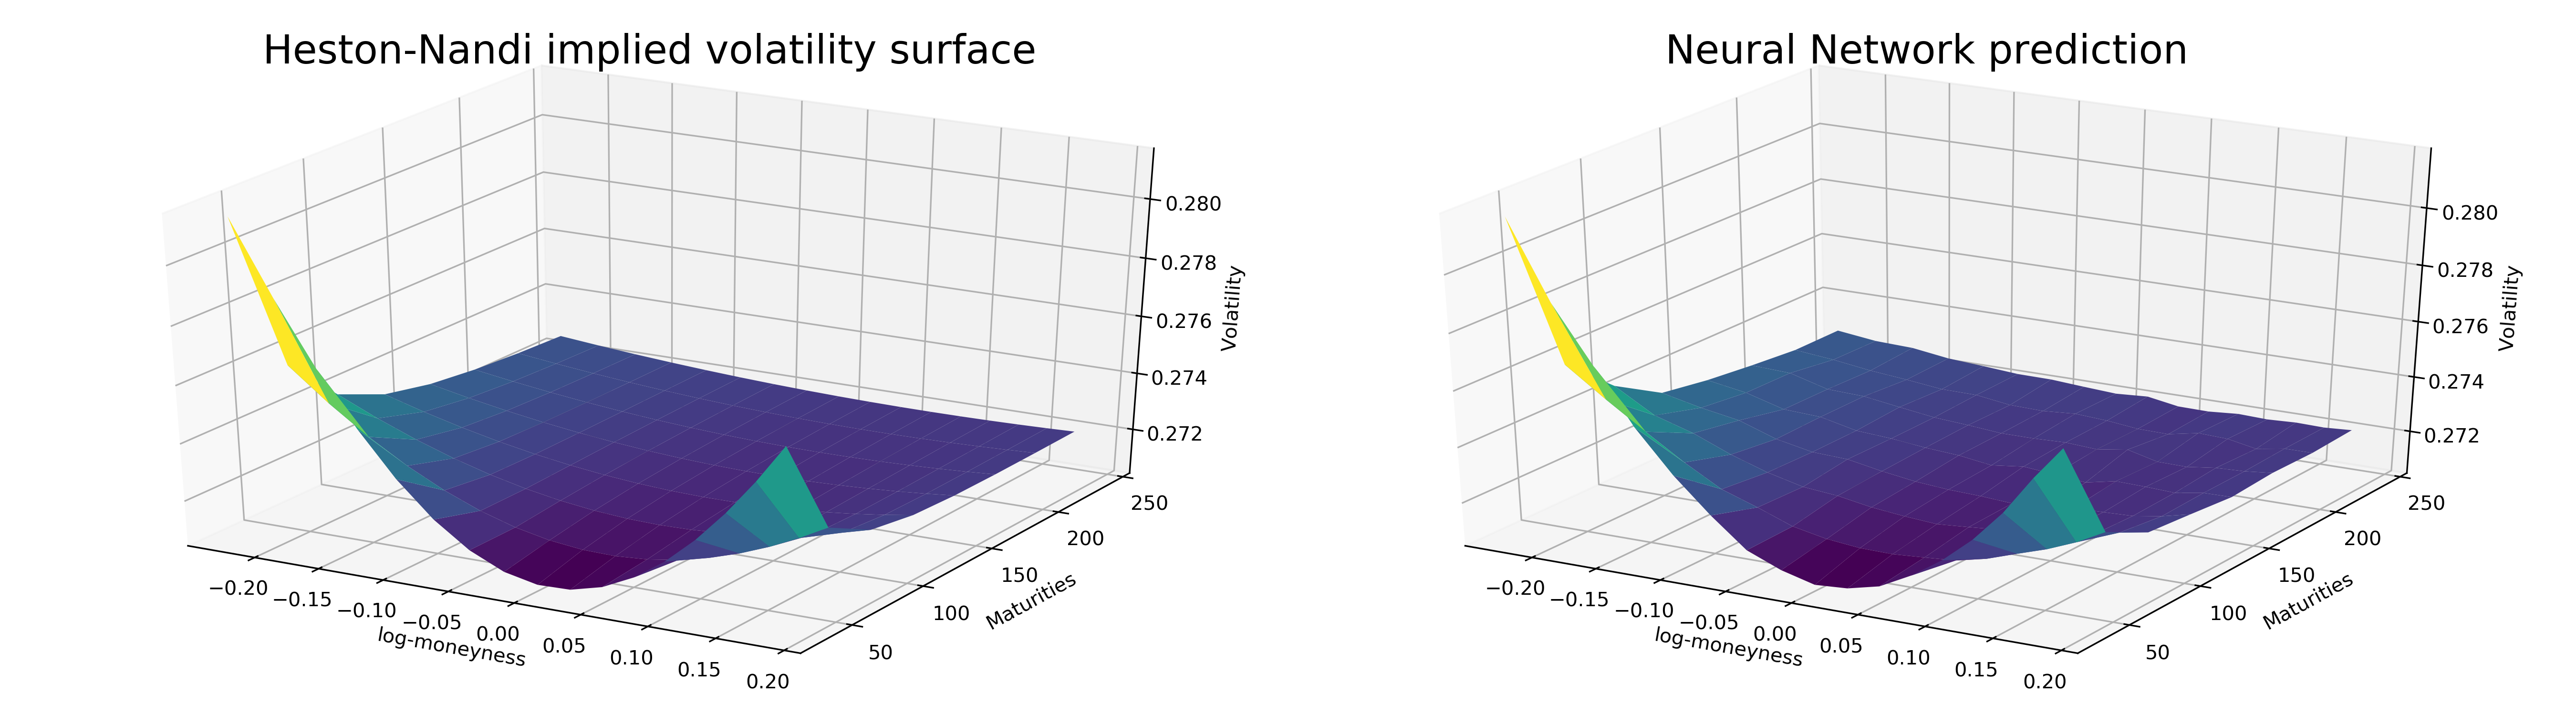
\includegraphics[width=\textwidth]{Small_g_Vola_surface.png}
\caption{Small $\gamma^*$ - comparison of volatility surface approximation by neural network to true surface}
\label{fig:Small_g_vola_surface}
\end{figure}
%=========================================================================
%Figure 10 Small g NN Parameter sensitivities
\begin{figure}[!ht]
\centering
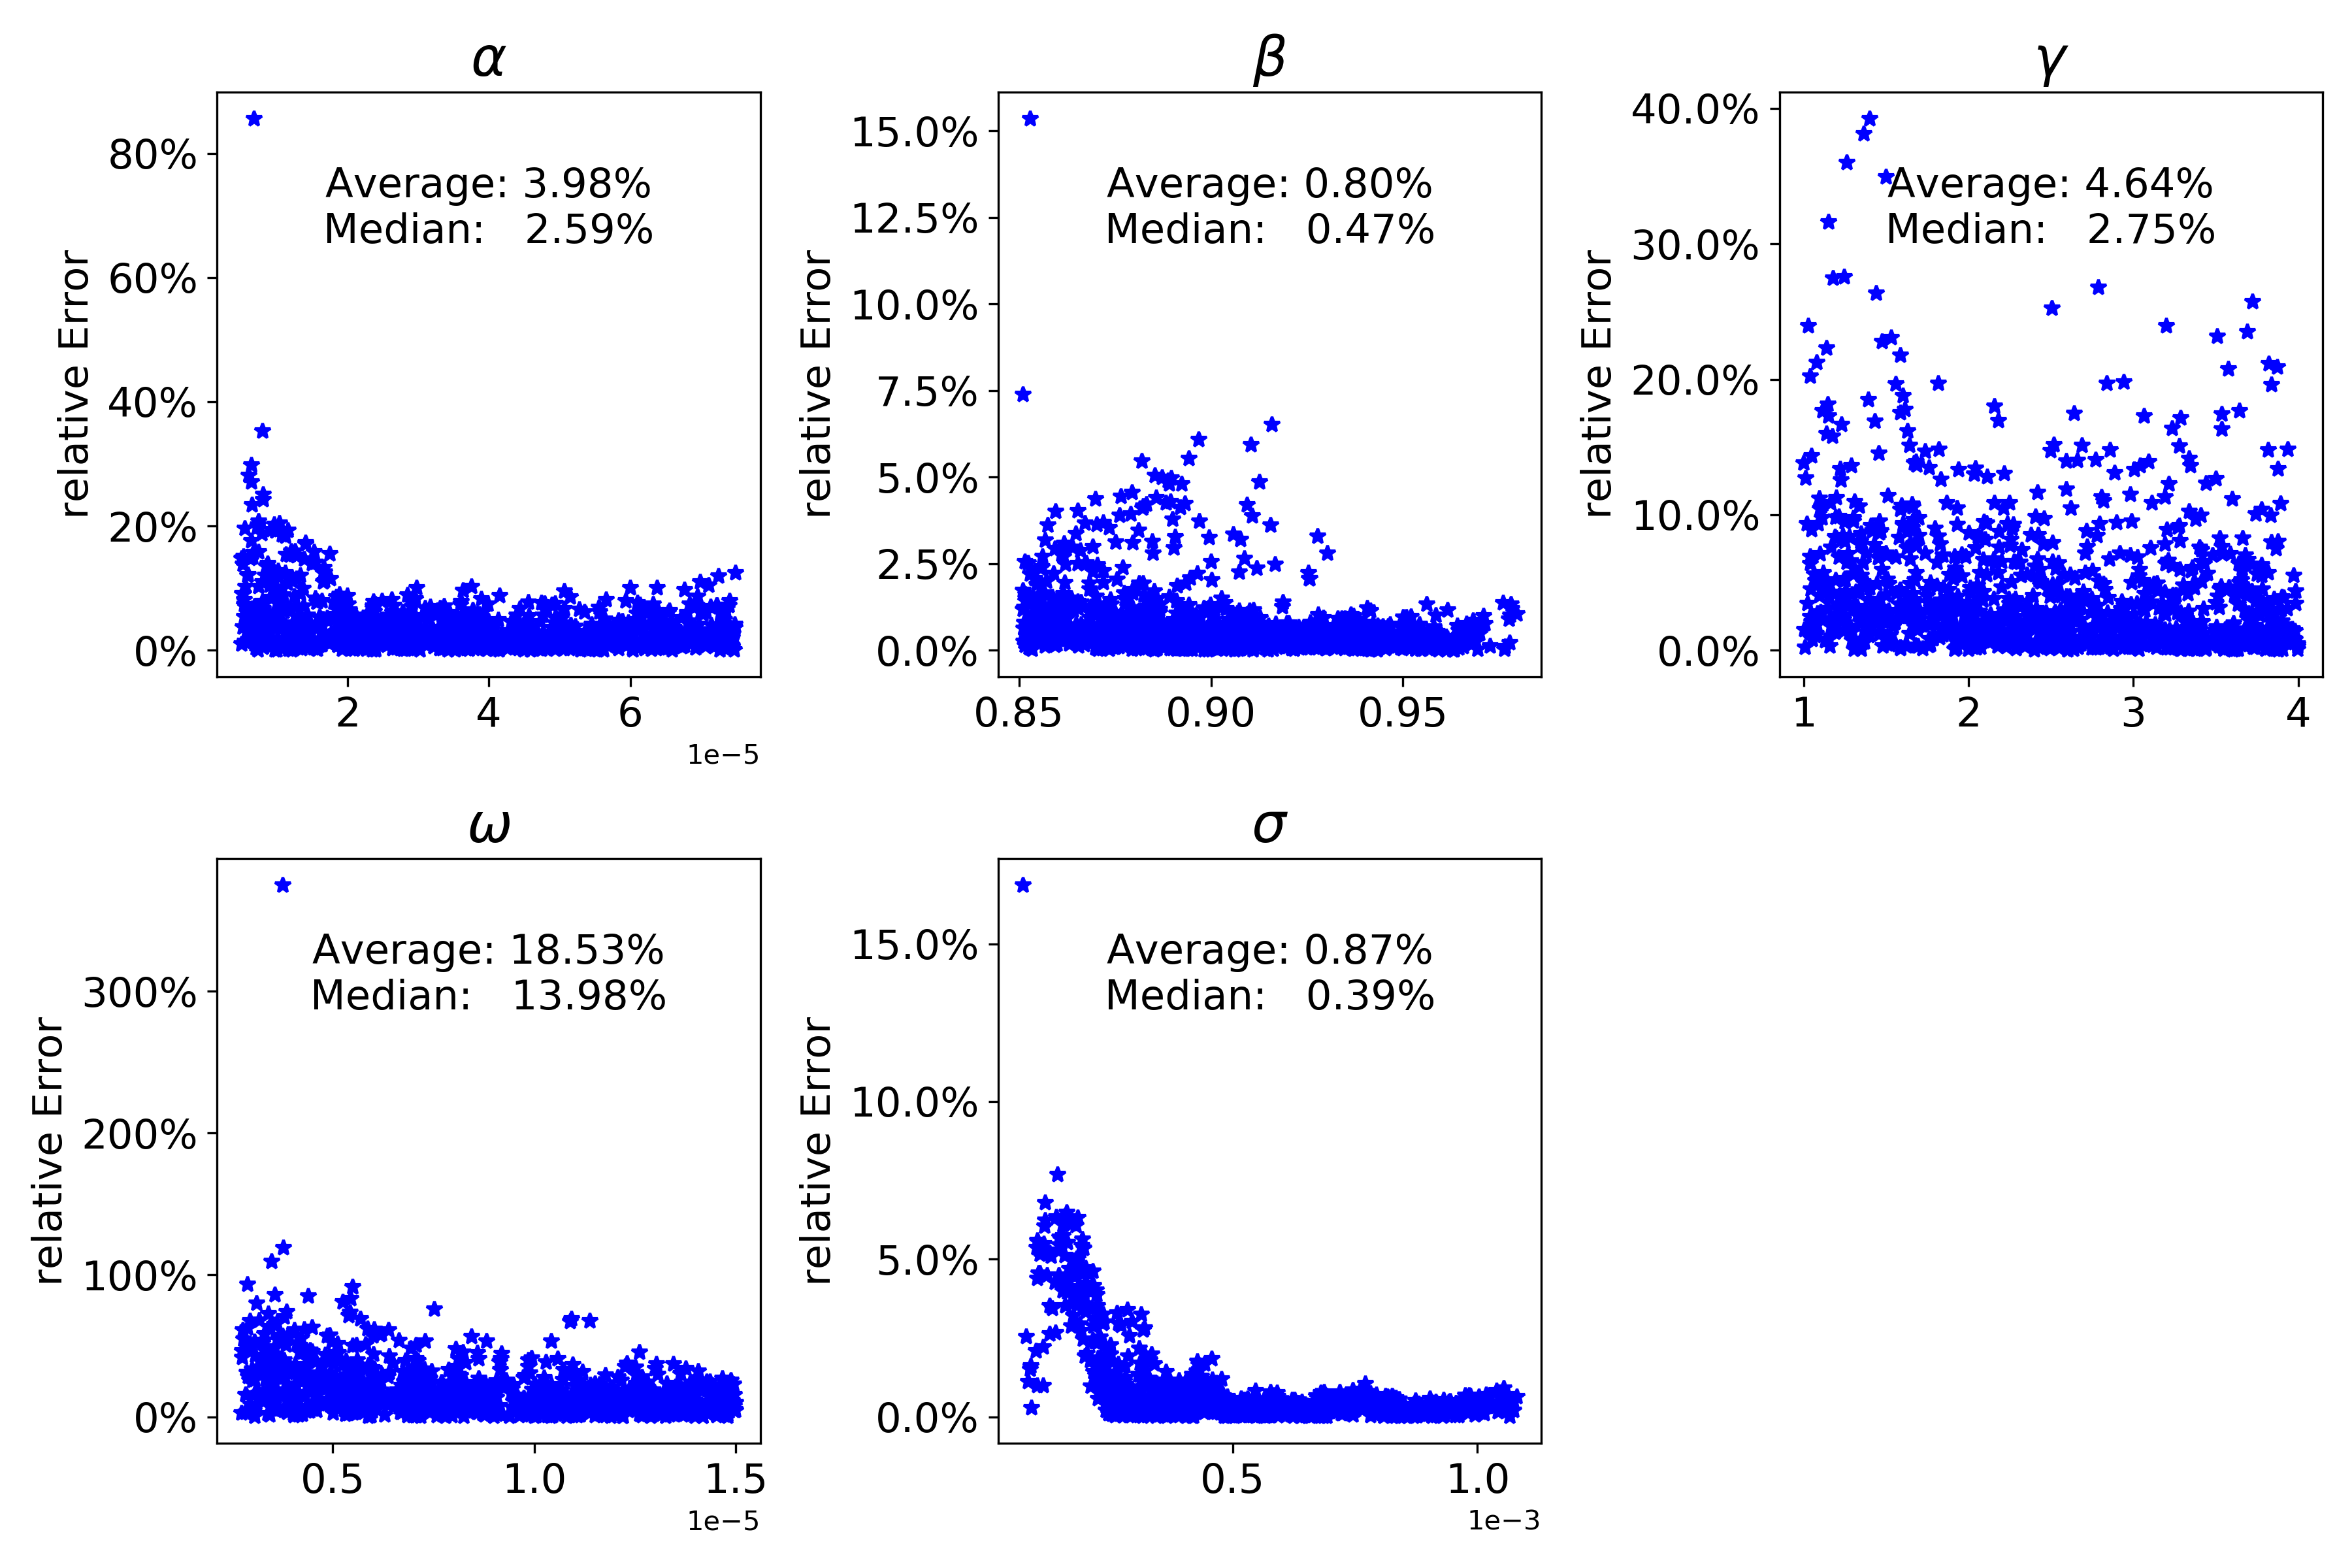
\includegraphics[width=\textwidth]{Small_g_Vola_HNG_ParameterRelativeErrors.png}
\caption{Small $\gamma^*$ - Relative errors of the parameters after calibration with Levenberg-Marquardt compared to true parameters in the test set}
\label{fig:Small_g_par_sen}
\end{figure}
%\fi %zum Auskommentieren
%=========================================================================

\subsection{Price surfaces}\label{sec:price_surf}
As the neural network performs pretty accurate at learning implied volatility surfaces we want to work out if it can also learn option prices directly. For that purpose we generate datasets according to Section \ref{sec:scenarios} but change the output to prices instead of implied volatilities. The obtained results along all three datasets are quite similar, so we just state them for the dataset with the small $\gamma^*$ parameters. \newline
Figure \ref{fig:Small_g_Price_NN_rel_err} indicates that the neural network learns the prices on the vast majority of the grid precisely but the upper right-hand corner is problematic. There the prices are smallest on the whole grid since the call option has only a short time to maturity left while is deep out of the money. We suspect that the price surface has a more complex datastructure than the implied volatilities. For example the implied volatilites in the small $\gamma^*$ dataset range from $0.12$ up to $0.53$ while the corresponding prices range from $1.1\cdot 10^{-6}$ up to $0.3$. Although we normalize these numbers we think that the much higher variability in the prices is more difficult for the net to handle. 


%=========================================================================
%Figure 11 Small g Prices NN relative errors
%\iffalse %zum Auskommentieren
\begin{figure}[!ht]
\centering
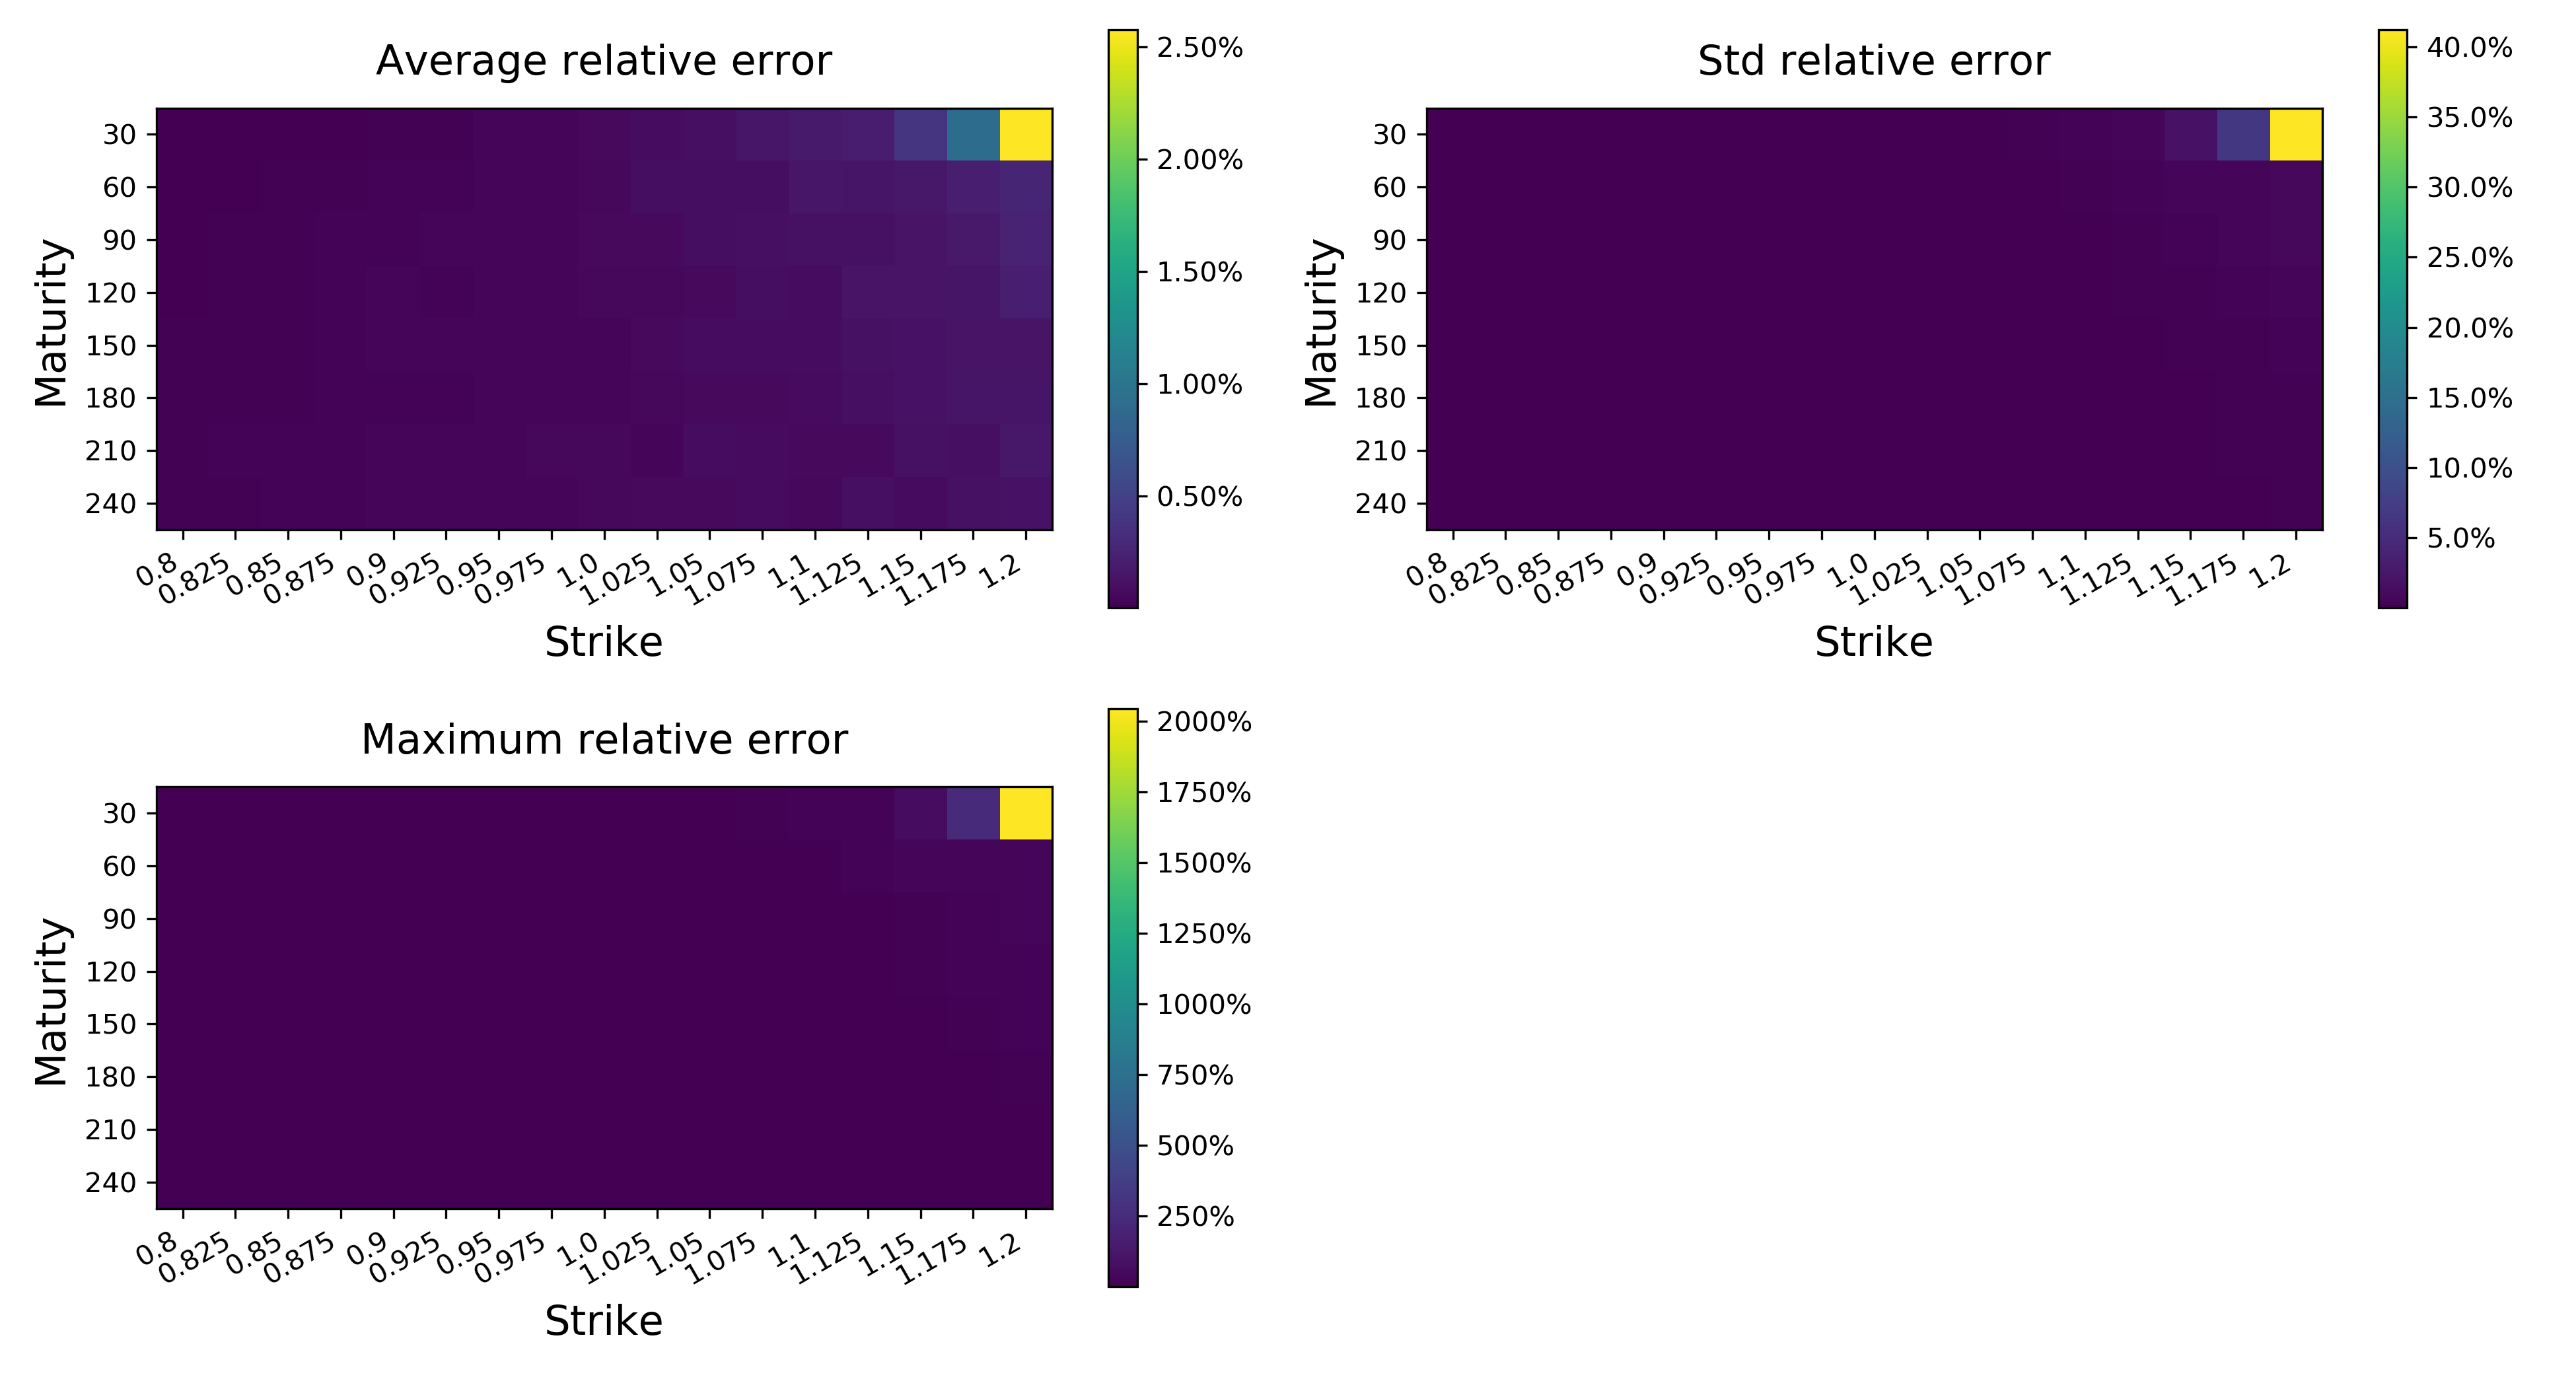
\includegraphics[width=\textwidth]{Small_g_Price_HNG_NNErrors.png}
\caption{Small $\gamma^*$ - Relative errors of the neural network predicted option prices compared to true prices in the test set}
\label{fig:Small_g_Price_NN_rel_err}
\end{figure}
%=========================================================================
%Figure 12 Small g Price surface
\begin{figure}[!ht]
\centering
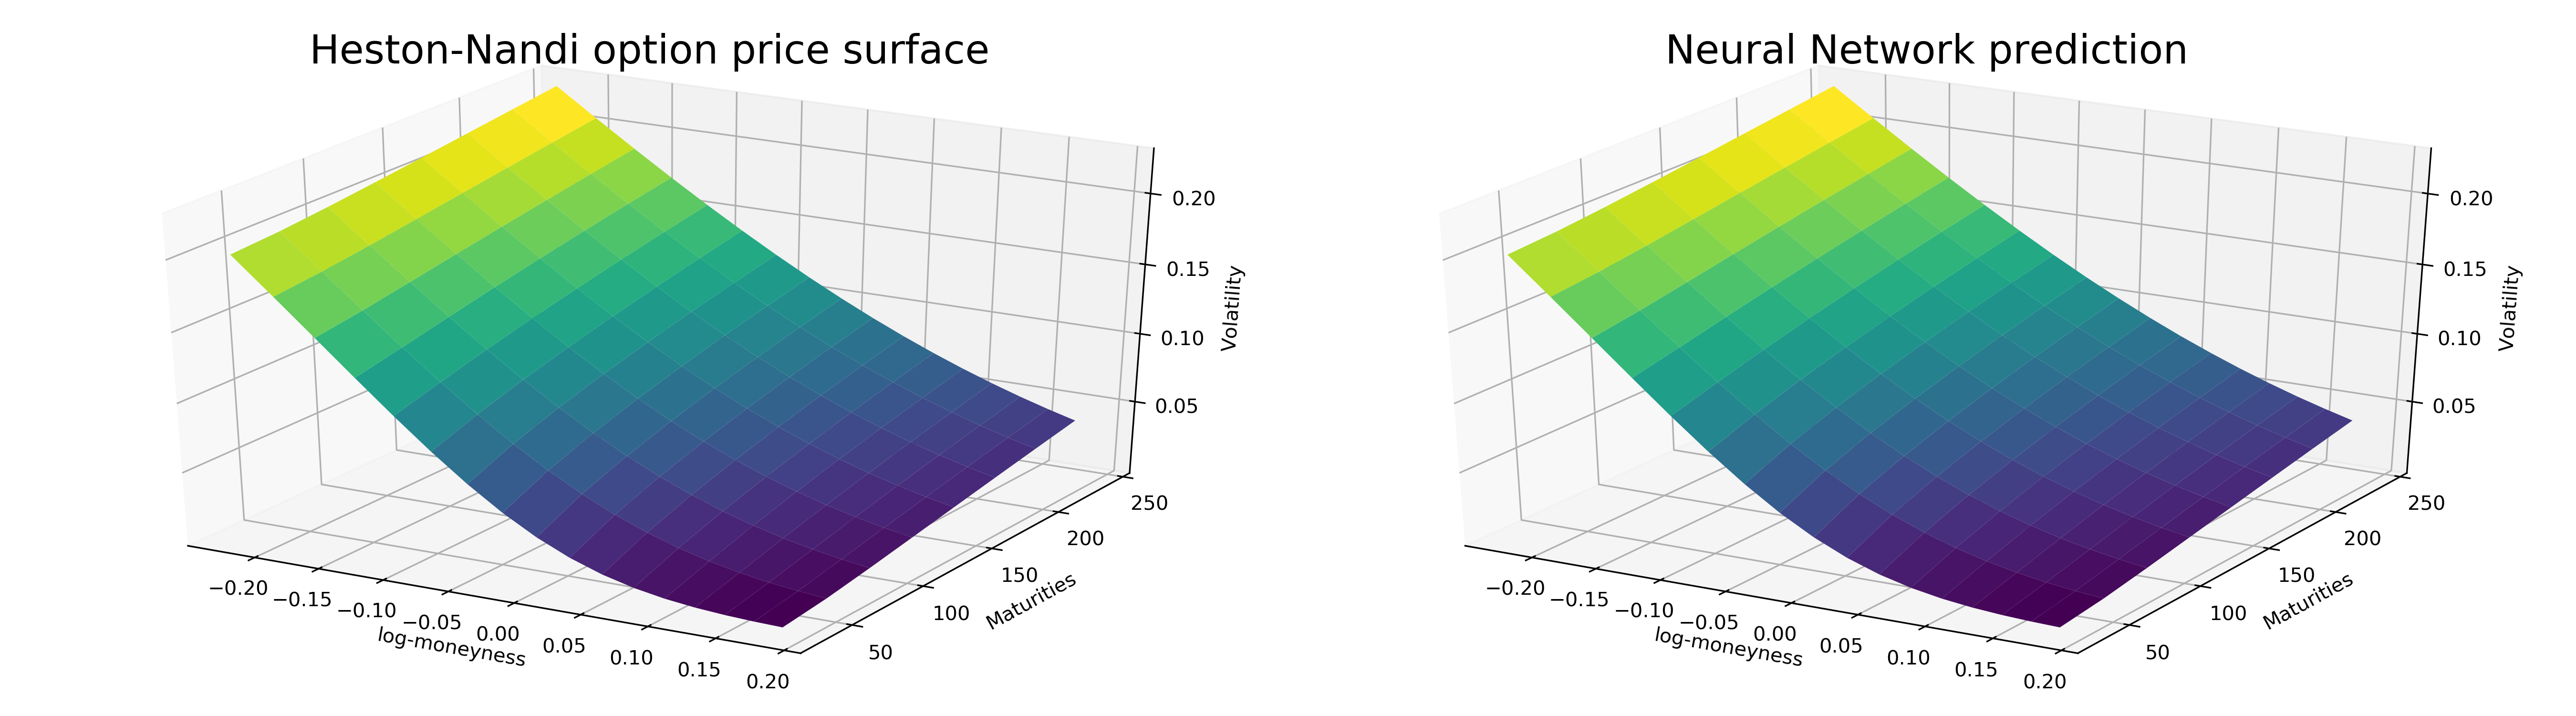
\includegraphics[width=\textwidth]{Small_g_Price_surface.png}
\caption{Small $\gamma^*$ - comparison of option price surface approximation by neural network to true price surface}
\label{fig:Small_g_price_surface}
\end{figure}
%\fi %zum Auskommentieren
%=========================================================================
\subsubsection{Performance in Comparsion to Black-Scholes}\label{sec:bs_results}
Even tho the fit on price surfaces looks promising, a small error itself does not guarantee a good performance of the learned network. Hence, we use the BS model as baseline. In each scenario the annualized expected volatility $\sigma_{year}=\sqrt{252\E(h_t)}$ is calculated and used as parameter for BS. The corresponding BS price surface is generated and the RMSE between BS model and HNG model as well as the RMSE between the neural net and HNG model is calculated. We find that in terms of RMSE our approach outperforms BS. The average RMSE is in the magnitude of $10^{-5}$ for the neural net while the average BS performance tends to be around $10^{-2}$ (cf. Table \ref{tab:bs_rmse}). We conclude that the neural net is indeed able to fit the HNG model precisely. Additional plots can be find in Appendix \ref{app:bs_rmse}.
\begin{table}[!ht]
\centering
\begin{tabular}{|l|l|l|l|l|l|l|}
\hline
\multirow{2}{*}{} & \multicolumn{2}{c|}{1\ts{st} Model \footnotemark} & \multicolumn{2}{c|}{2\ts{nd} Model \footnotemark} & \multicolumn{2}{c|}{3\ts{rd} Model \footnotemark} \\ \cline{2-7} 
 & \multicolumn{1}{c|}{NN} & \multicolumn{1}{c|}{BS} & \multicolumn{1}{c|}{NN} & \multicolumn{1}{c|}{BS} & \multicolumn{1}{c|}{NN} & \multicolumn{1}{c|}{BS} \\ \hline
\multicolumn{1}{|c|}{Average} & 1.700e-5 & 6.549e-2 & 3.944e-6 & 5.412e-2 & 1.271e-5 & 9.947e-2 \\ \hline
\multicolumn{1}{|c|}{Standard Deviation} & 7.520e-6 & 7.578e-3 & 1.228e-6 & 1.902e-3 & 4.534e-6 & 5.001e-3 \\ \hline
\end{tabular}\label{tab:bs_rmse}\vspace{0.1cm}
\caption{Performance Analysis - RMSE in each setup}
\end{table}
\footnotetext[5]{corresponds to the setup in \ref{sec:setupmle}}
\footnotetext[6]{corresponds to the setup in \ref{sec:setupomega20}}
\footnotetext[7]{corresponds to the setup in \ref{sec:setupsmallg}}
\subsection{Outlook: "How to involve real data"}
\label{sec:results_sp500}
As mentioned in Section \ref{sec:real_data} it is desirable not only to fit a model precisely but to use the neural net for real data. We take the real call option price surface of different years and treat them as test samples. Then we test how precise the trained neural network can rebuild these real price surfaces. The neural network is trained on the 90\% MLE estimator dataset. So far this is just a rough idea and not an optimized procedure. One need to keep in mind that neither the option prices are analysed on their properties (e.g. whether some of them allow arbitrage and should be excluded) nor parameters and neural net are able to adjust for a differences in real risk free rates. Additionally, the errors explode in the upper right-hand corner (cf. Figure \ref{fig:MLE_Price_NN_rel_err}) consistent with the findings in Section \ref{sec:price_surf}.    
%=========================================================================
%Figure 13 MLE Prices NN relative errors compared to Sp500
%\iffalse %zum Auskommentieren
\begin{figure}[!ht]
\centering
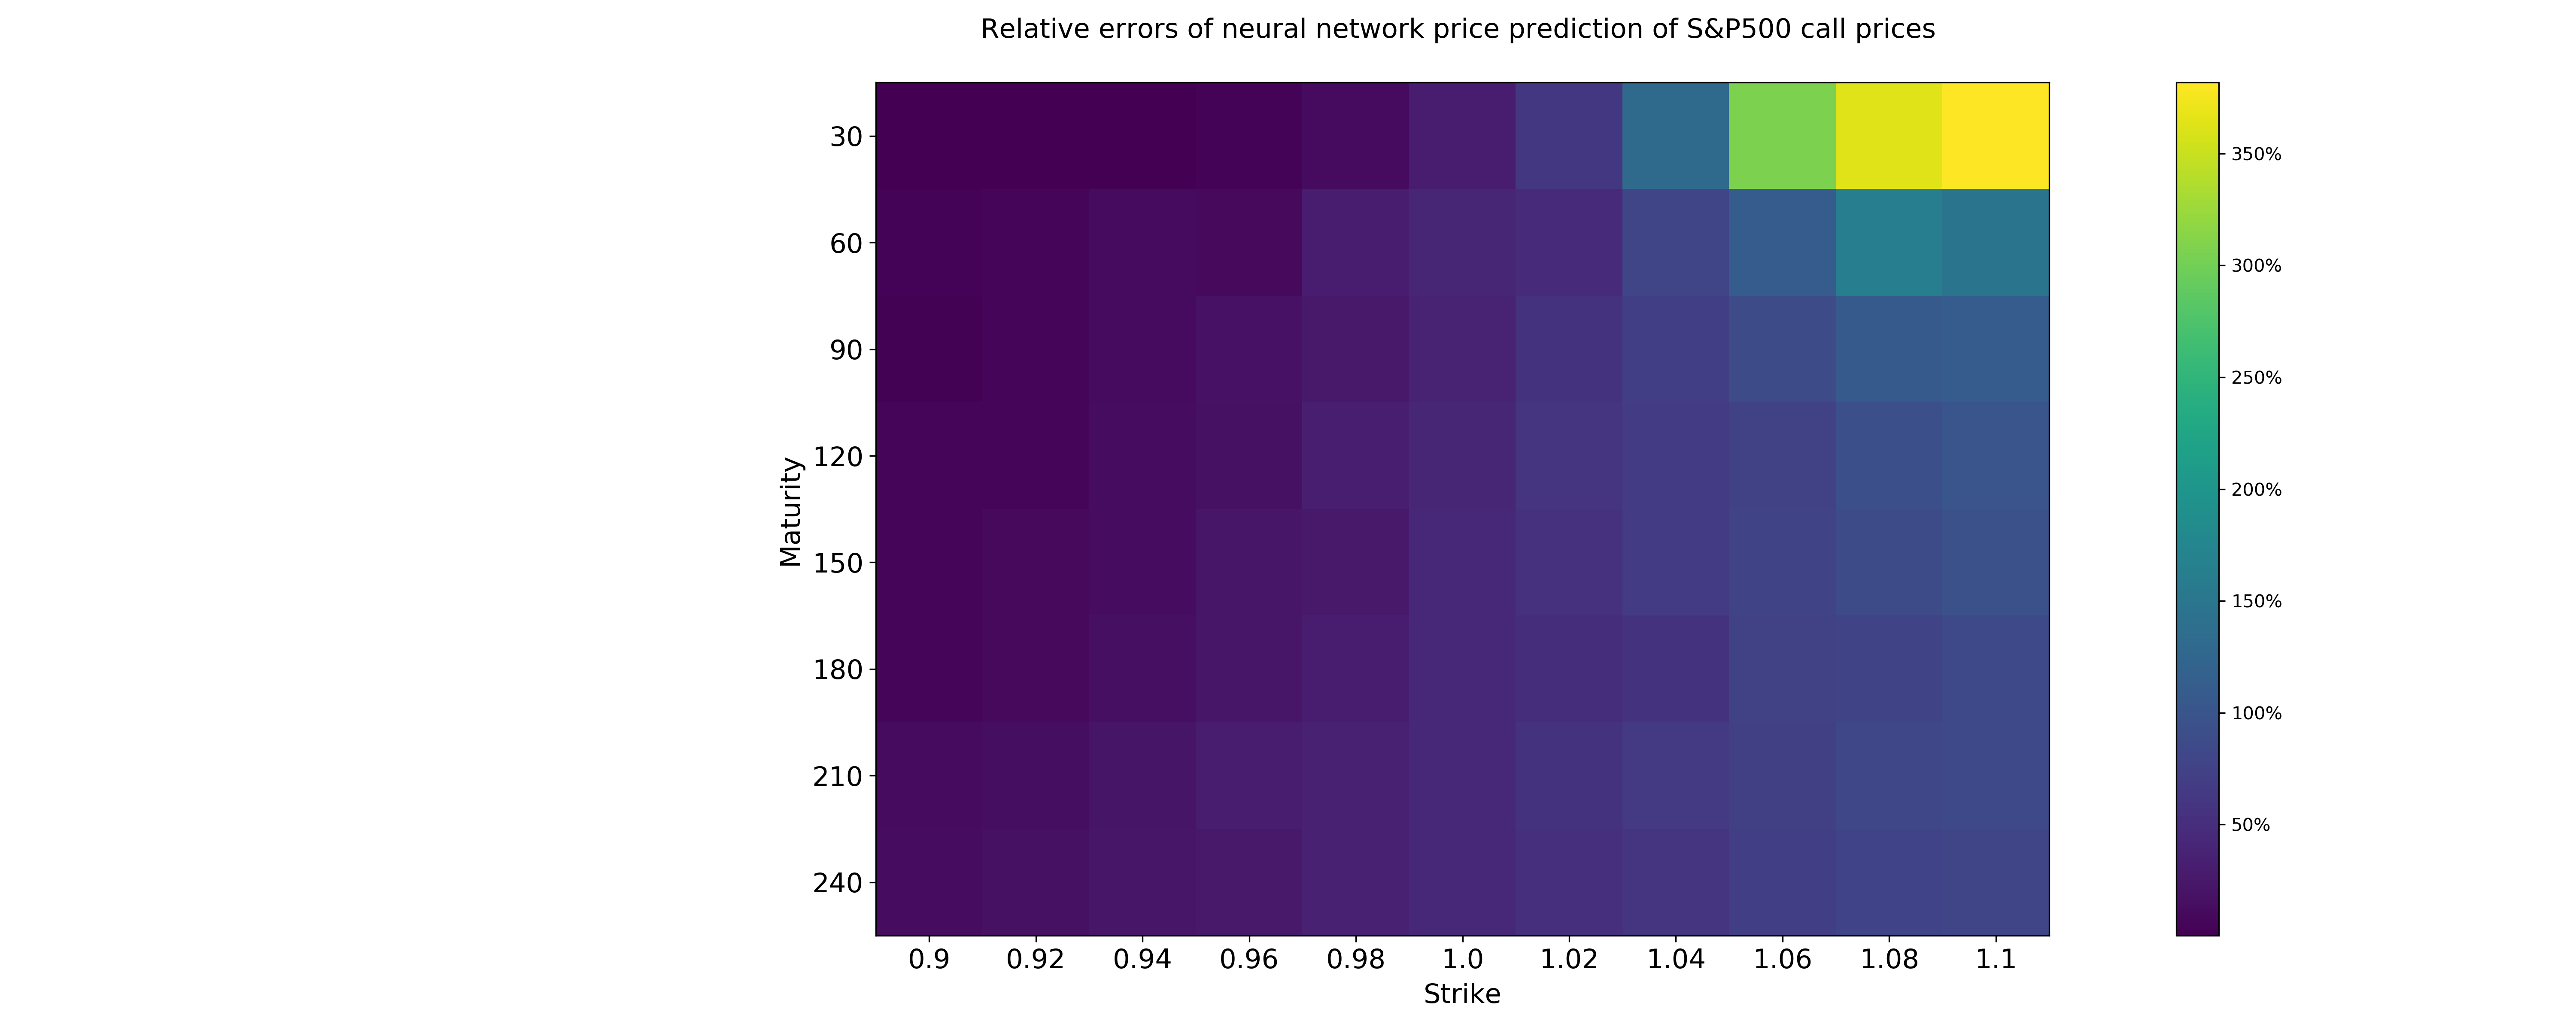
\includegraphics[width=\textwidth]{MLE_Price_NN_err_Sp500.png}
\caption{Relative errors of the neural network predicted option prices compared to true S\&P500 prices in 2013}
\label{fig:MLE_Price_NN_rel_err}
\end{figure}
%\fi %zum Auskommentieren
%=========================================================================
So far this approach does not outperform option pricing with standard techniques like BS. We are confident that these challenges can be overcome in the future.

\subsection{Robustness}
\subsubsection{Sensitivity towards mispricing}

At a first test we want to carry out how sensitive the neural net reacts to small changes in the output data (volatilities).  For this purpose we take the dataset generated according to Section \ref{sec:setupomega20}. Thereafter we add a $\pm 1\%$ uniform distributed noise to the implied volatilities in the train and validation set and compare the performance of the neural net on the test set to the net initialized by the original train and validation data. On average the noised volatilities lead to 137\% higher mean relative errors than the pure volatilities in the test set. Also the maximum relative error is 144\% higher. The calibrated parameters have on average a 56\% higher median relative error than the parameters calibrated based on the pure dataset. \newline
The results indicate that a precise calculation of call option implied volatilities e.g. via a closed-form solution rather than Monte Carlo simulation significantly increase the performance of the two step calibration approach.
%=========================================================================
%Figure 14 low relative error dataset add noise to volatilities in train set
%\iffalse %zum Auskommentieren
\begin{figure}[!ht]
\centering
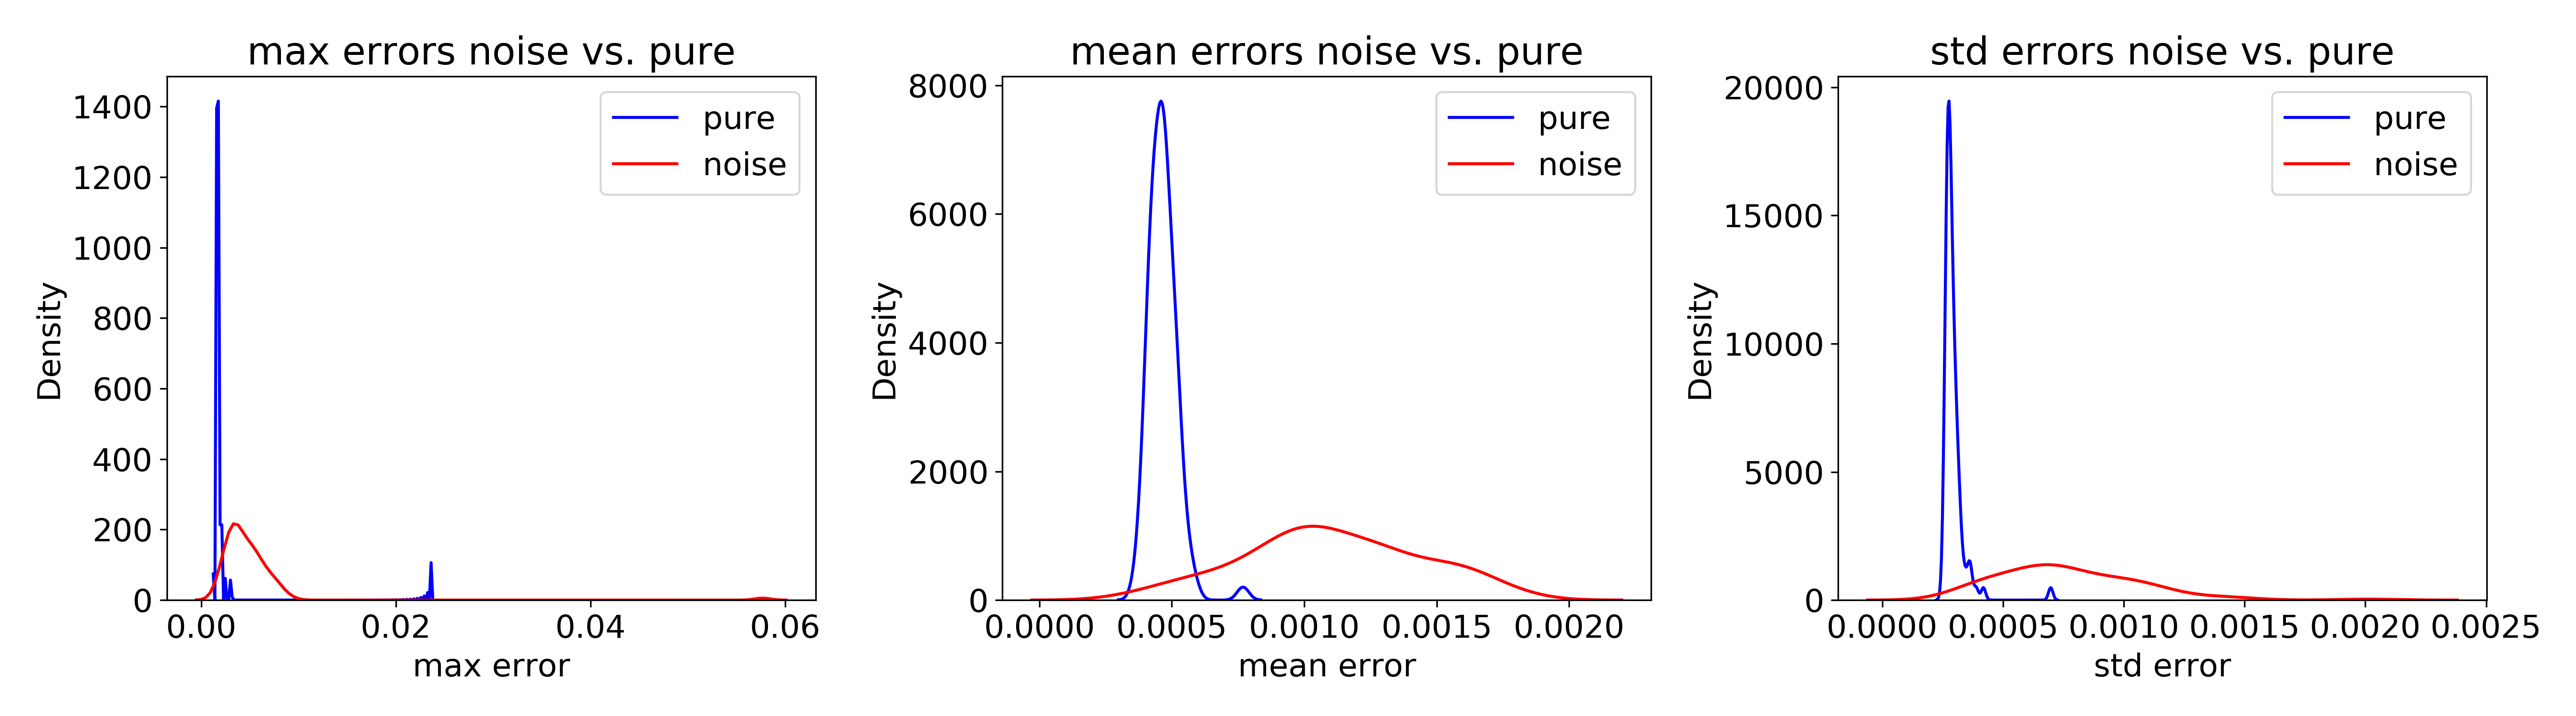
\includegraphics[width=\textwidth]{Robustness_Vola_Noise.png}
\caption{Robustness test for the best fit dataset (cf. Section \ref{sec:setupomega20}) - pure dataset vs. dataset with $\pm 1\%$ noise in the train set volatilities}
\label{fig:MLE_Price_NN_rel_err}
\end{figure}
%\fi %zum Auskommentieren
%=========================================================================


\subsubsection{Sensitivity towards training set size} \label{sec:robust_size}
So far our findings imply that the performance is highly dependent on the quality of the generated training set. Additionally, it is important to check the sensitivity of the results towards the size of a training set. For doing so, we fix a given test set but decrease the size of training and validation set randomly by 40\%. This procedure is repeated 20 times. The change in error-distribution can be seen in Figure
\ref{fig:trainset_sensitivity}.
%=============================================================
%\iffalse
\begin{figure}[!ht]
    \centering
    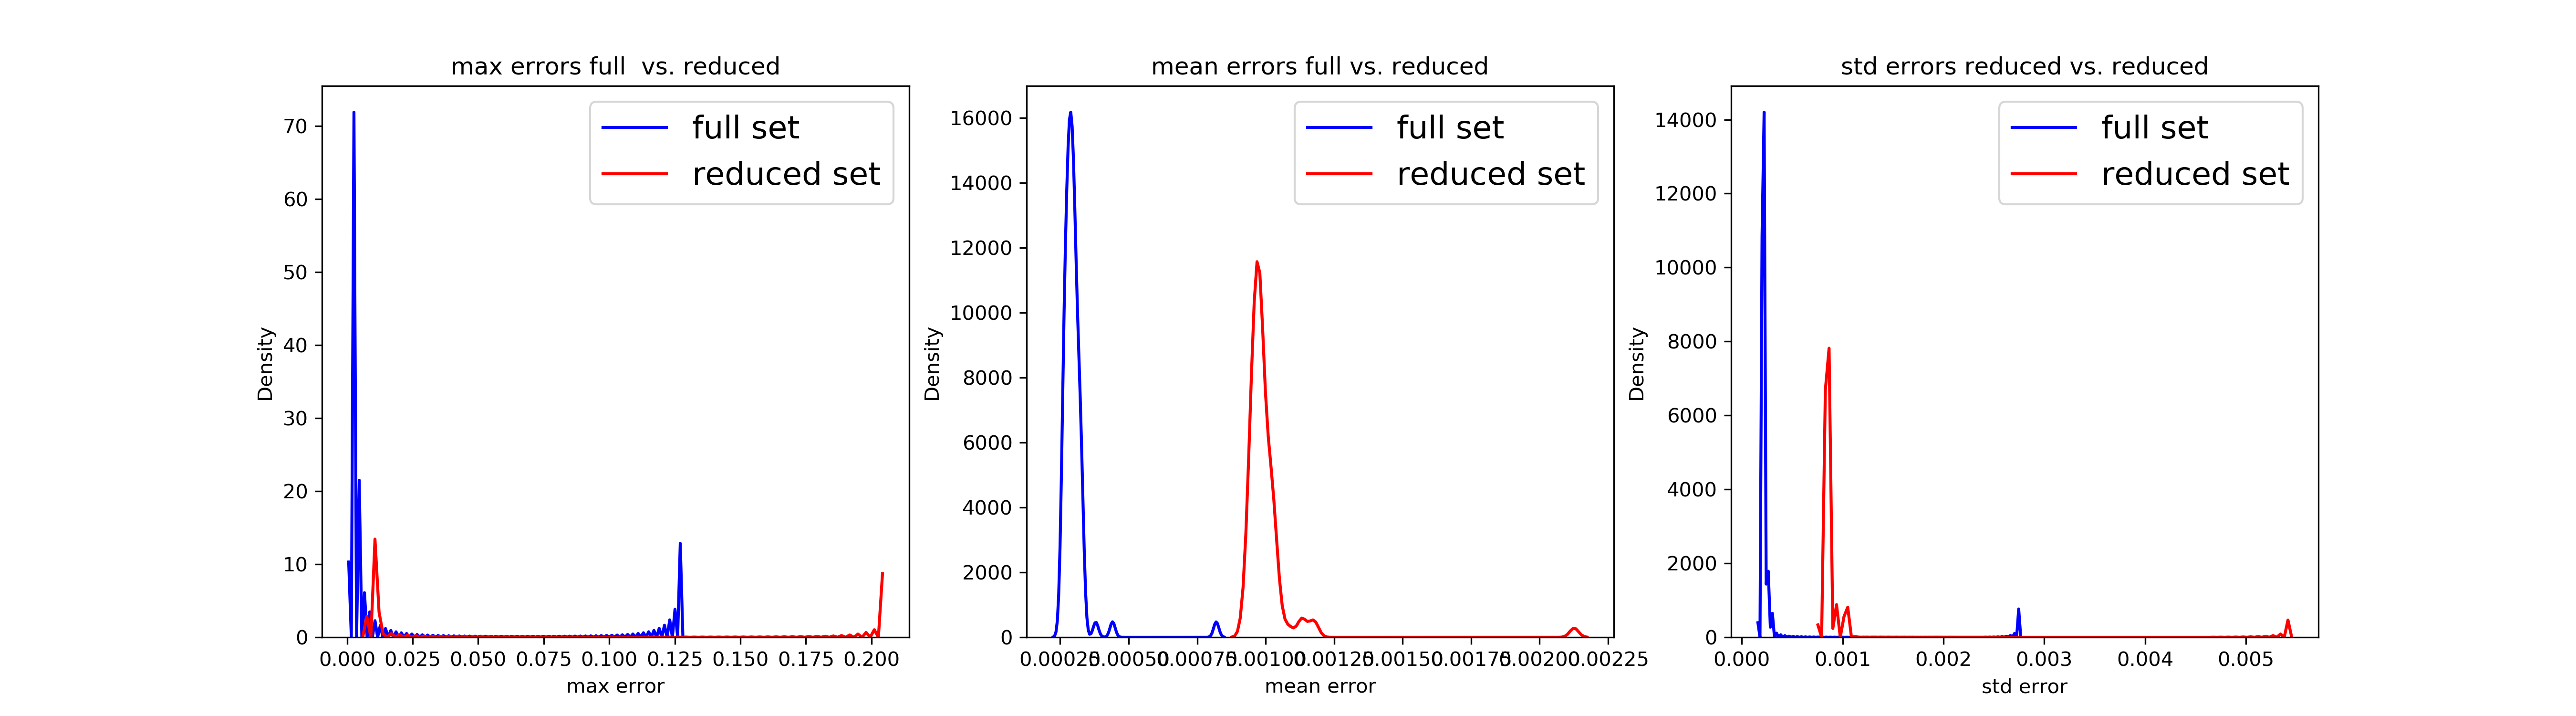
\includegraphics[width=\textwidth]{RobustnessSize.png}
    \caption{Robustnesstest - Change in size of training set}
    \label{fig:trainset_sensitivity}
\end{figure}
%\fi
%============================================================
  \\ 
The size reduction leads to an increase of mean relative error of 233.9\%. The maximal relative error increases by  59.8\%.  Furthermore the distribution of weights in the neural net is compared. 2-sample Kolmogorv-Smirnoff tests indicate significant change in distribution of weights in same layers (cf. Table \ref{tab:weights_size}. 
\begin{table}[!ht]
    \centering
    \begin{tabular}{|r|c|c|c|c|}\hline
     & Layer 1     &  Layer 2     & Layer 3 &    Output\\\hline
    avg. p-val & 2.162e-1 & 1.404e-1& 4.273e-1& 6.975e-6***\\\hline
    med. p-val & 1.672e-1 & 4.769e-2**& 3.772e-1& 2.708e-12***\\\hline
    max. p-val & 6.069e-1 & 5.342e-1& 9.653e-1& 6.194e-5***\\\hline
    \end{tabular}\vspace{0.1cm}
    \caption{2-Sample-KS-test - Comparison of weights in Neural Nets}
    \label{tab:weights_size}
\end{table}\\
The results of a 20\% size reduction are stated in Appendix \ref{app:robust_size}.
We conclude that the neural net approach does depend on the size of the training set. Even tho the performance significantly decreases 
in terms of prediction accuracy, it's surprising to see only small changes in the distribution of weights.
\section{Challenges and Discussion}
The most time consuming part of our research was the preparation of a well-balanced artificial dataset. Particularly we tried a lot to understand the dependencies between the parameters and their influence on the shape of the volatility surface. The parameters selected out of the intervals need to fulfil certain requirements like the stationarity constraint. They shouldn't lead to numerical errors at the implied volatility calculation and the resulting surfaces need to be learnable by the neural network, too. To accomplish these task guidelines to determine meaningful parameter intervals are helpful. This might be subject of further research.\\
Similar to Horvath et al. \cite{Blanka} the neural network also struggles with the approximation of the corner points on the strike-maturity grid even though our grids don't contain strikes smaller than 0.8  and larger than 1.2. The effect is intensified if price surfaces are considered (cf. Section \ref{sec:price_surf})  \\
Another subject for further research would be to emphasize the topic of real data. The greatest challenge there is again the choice of parameter intervals which gives the neural network the opportunity to learn the volatility surface implied by real data. Especially, we are not able to reproduce the particularly pronounced smile with Heston-Nandi-GARCH so far. Instead our volatility smiles are too flat. 
\section{Conclusion}
We find that the approach of Horvath et al. \cite{Blanka} is generalizable to discrete-time models. A neural net is able to outperform Black-Scholes in fitting the Heston-Nandi model. However, the accuracy of the trained net is highly dependent on the choice of training set. Parameter choice as well as the estimation accuracy are crucial to ensure a good performance. We provide a first idea on implementing real S\&P500, but calibration and fine tuning of this approach is subject to further research. 
\begin{thebibliography}{9}
\bibitem{Blanka}Horvath, B., Muguruza, A. and Tomas, M., 2019. Deep learning volatility. Available at SSRN 3322085.
\bibitem{HestonNandi}Heston, S.L. and Nandi, S., 2000. A closed-form GARCH option valuation model. The review of financial studies, 13(3), pp.585-625.
\bibitem{EngleGARCH}Engle, R.F., 1982. Autoregressive conditional heteroscedasticity with estimates of the variance of United Kingdom inflation. Econometrica: Journal of the Econometric Society, pp.987-1007.
\bibitem{HestonNandi97} Heston, S.L. and Nandi, S., 1997. A closed-form GARCH option pricing model.
\bibitem{GARCH}Hansen, P.R. and Lunde, A., 2005. A forecast comparison of volatility models: does anything beat a GARCH (1, 1)?. Journal of applied econometrics, 20(7), pp.873-889.
\bibitem{Book}Chorro, C., Guégan, D. and Ielpo, F., 2015. A Time Series Approach to Option Pricing: Models, Methods and Empirical Performances, 2015th edn, Springer, Berlin, Heidelberg.
\bibitem{Hernandez}Hernandez, A., 2017. Model calibration with neural networks. Risk.
%not used yet
\bibitem{BlankaRef37}Horvath, B., Jacquier, A. and Muguruza, A., 2017. Functional central limit theorems for rough volatility. Available at SSRN 3078743.
\bibitem{LyudmilaJuanPaplo}Badescu1, A., Grigoryeva, L., and Ortega, J., 2019. Option pricing and hedging with one-step unscented Kalman filtered factors in non-affine stochastic volatility models. Working Paper
\bibitem{PavelMaster} Podkovyrov, P., 2019. Option Pricing Using Machine Learning Techniques. Master Thesis University of Konstanz, Germany.
\bibitem{StudyHestonNandi} Byun, S.J., 2011. A Study on Heston-Nandi GARCH Option Pricing Model. KAIST Business
School, Korea.
\end{thebibliography}\newpage
\section*{Appendix}
\appendix

\section{Further Volatility Plots}\label{sec:app_vola_plots}
This section shows furhter volatility plots and error analysis for Chapter \ref{sec:vola_results}
%=========================================================================
%Figure A1 MLE CDF errors
%\iffalse  %zum Auskommentieren
\begin{figure}[!ht]
\centering
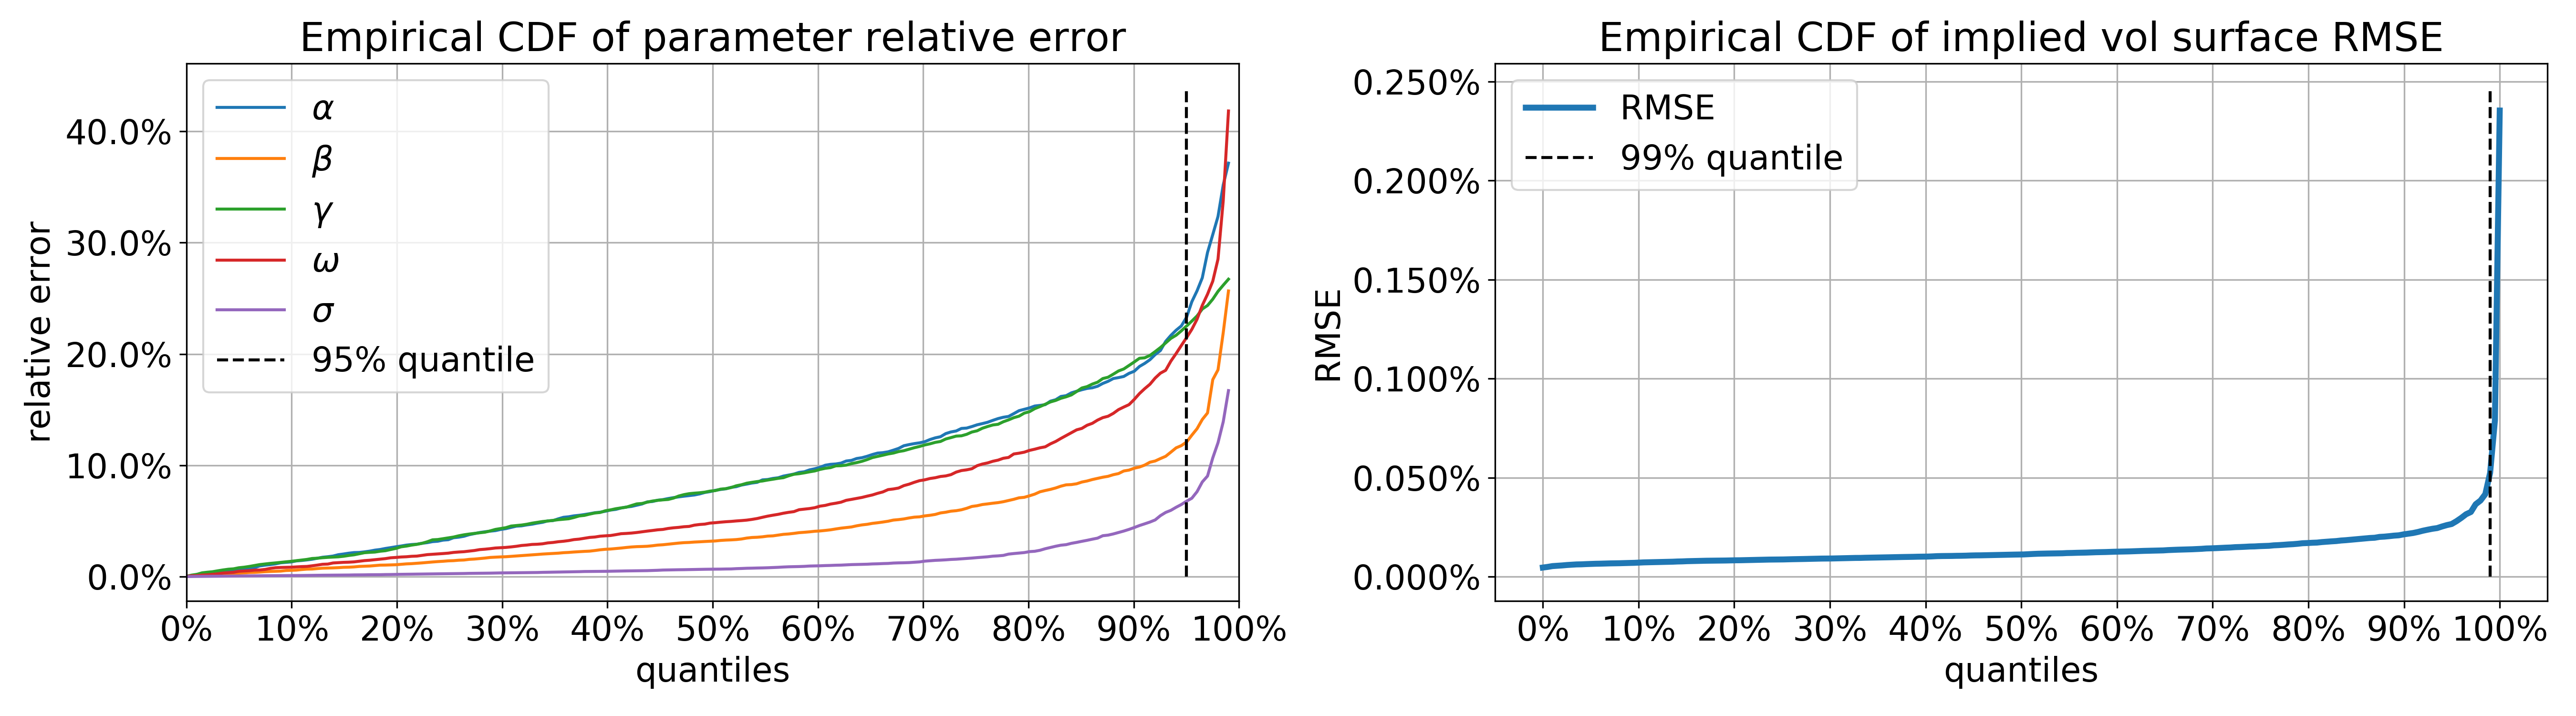
\includegraphics[width=\textwidth]{MLE_Vola_HNG_ErrorCDF.png}
\caption{$90\%$ Maximum Likelihood confidence interval - Empirical CDF of parameter relative error and empirical CDF of implied volatility surface RMSE}
\label{fig:MLE_CDF}
\end{figure}
%=========================================================================
%Figure A2 Low error CDF errors
\begin{figure}[!ht]
\centering
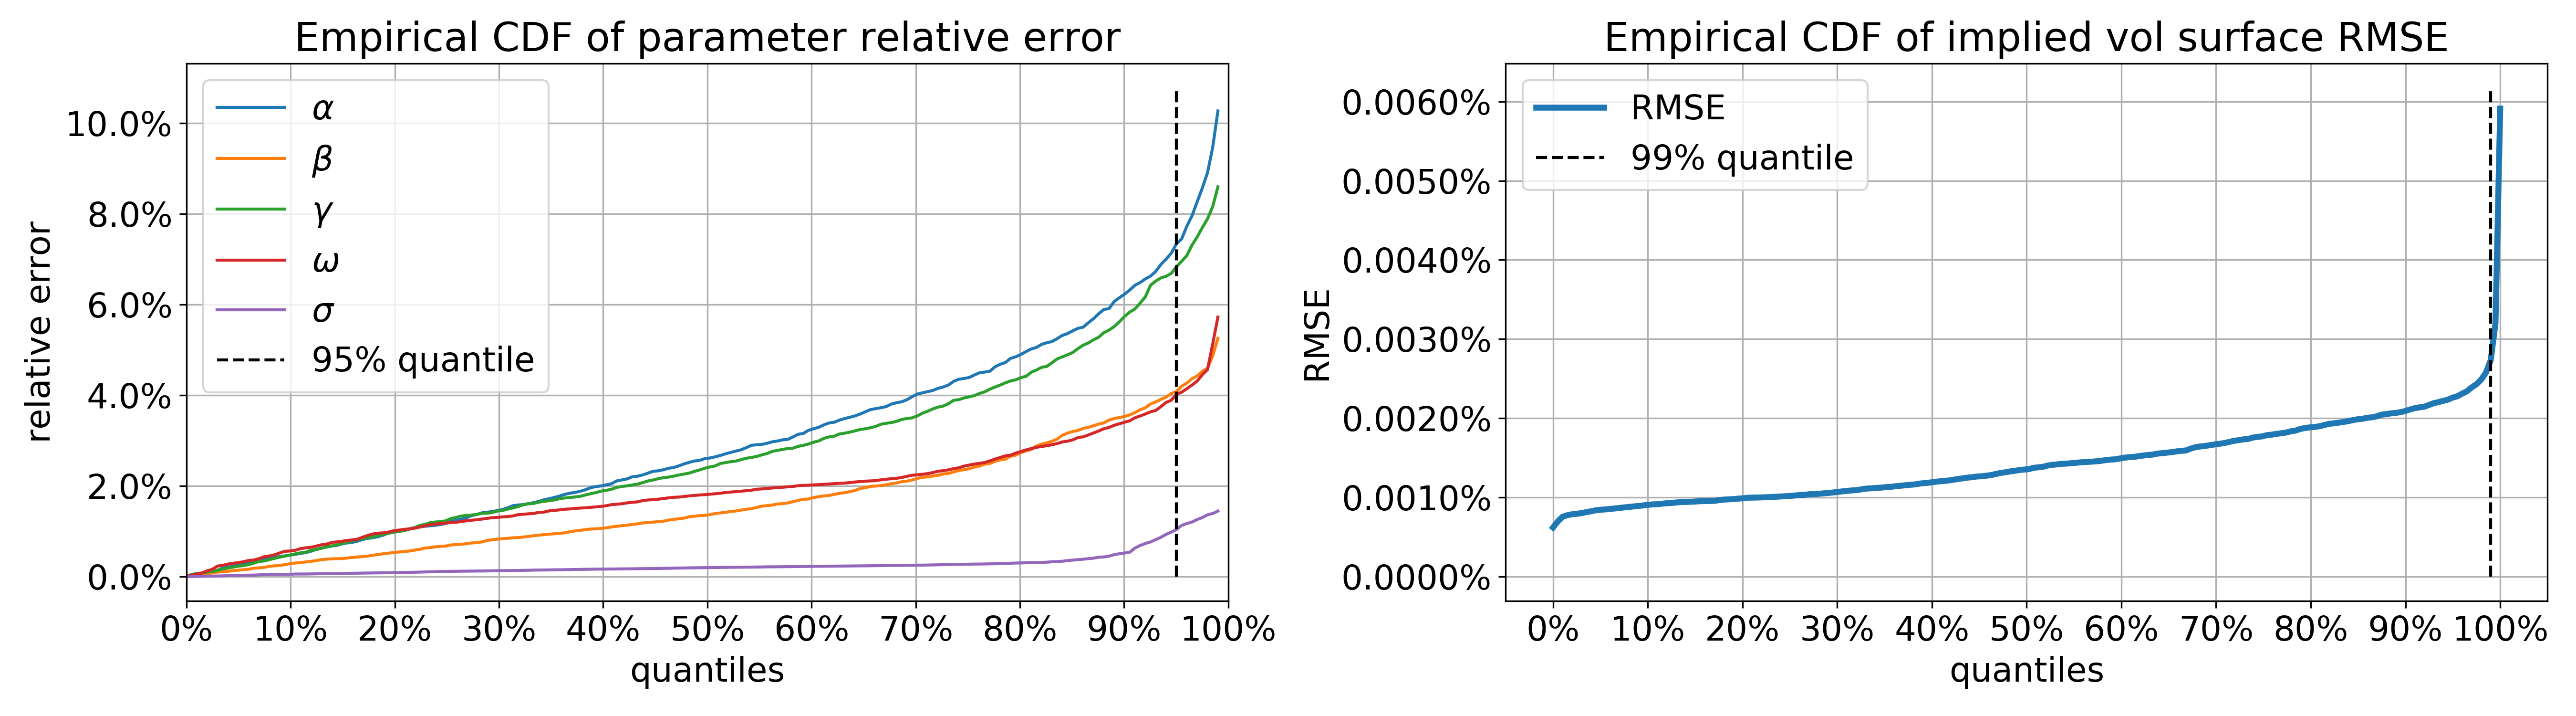
\includegraphics[width=\textwidth]{Low_error_HNG_ErrorCDF.png}
\caption{Best fit - Empirical CDF of parameter relative error and empirical CDF of implied volatility surface RMSE}
\label{fig:low_err_CDF}
\end{figure}
%=========================================================================
%Figure A3 Small g CDF errors
\begin{figure}[!ht]
\centering
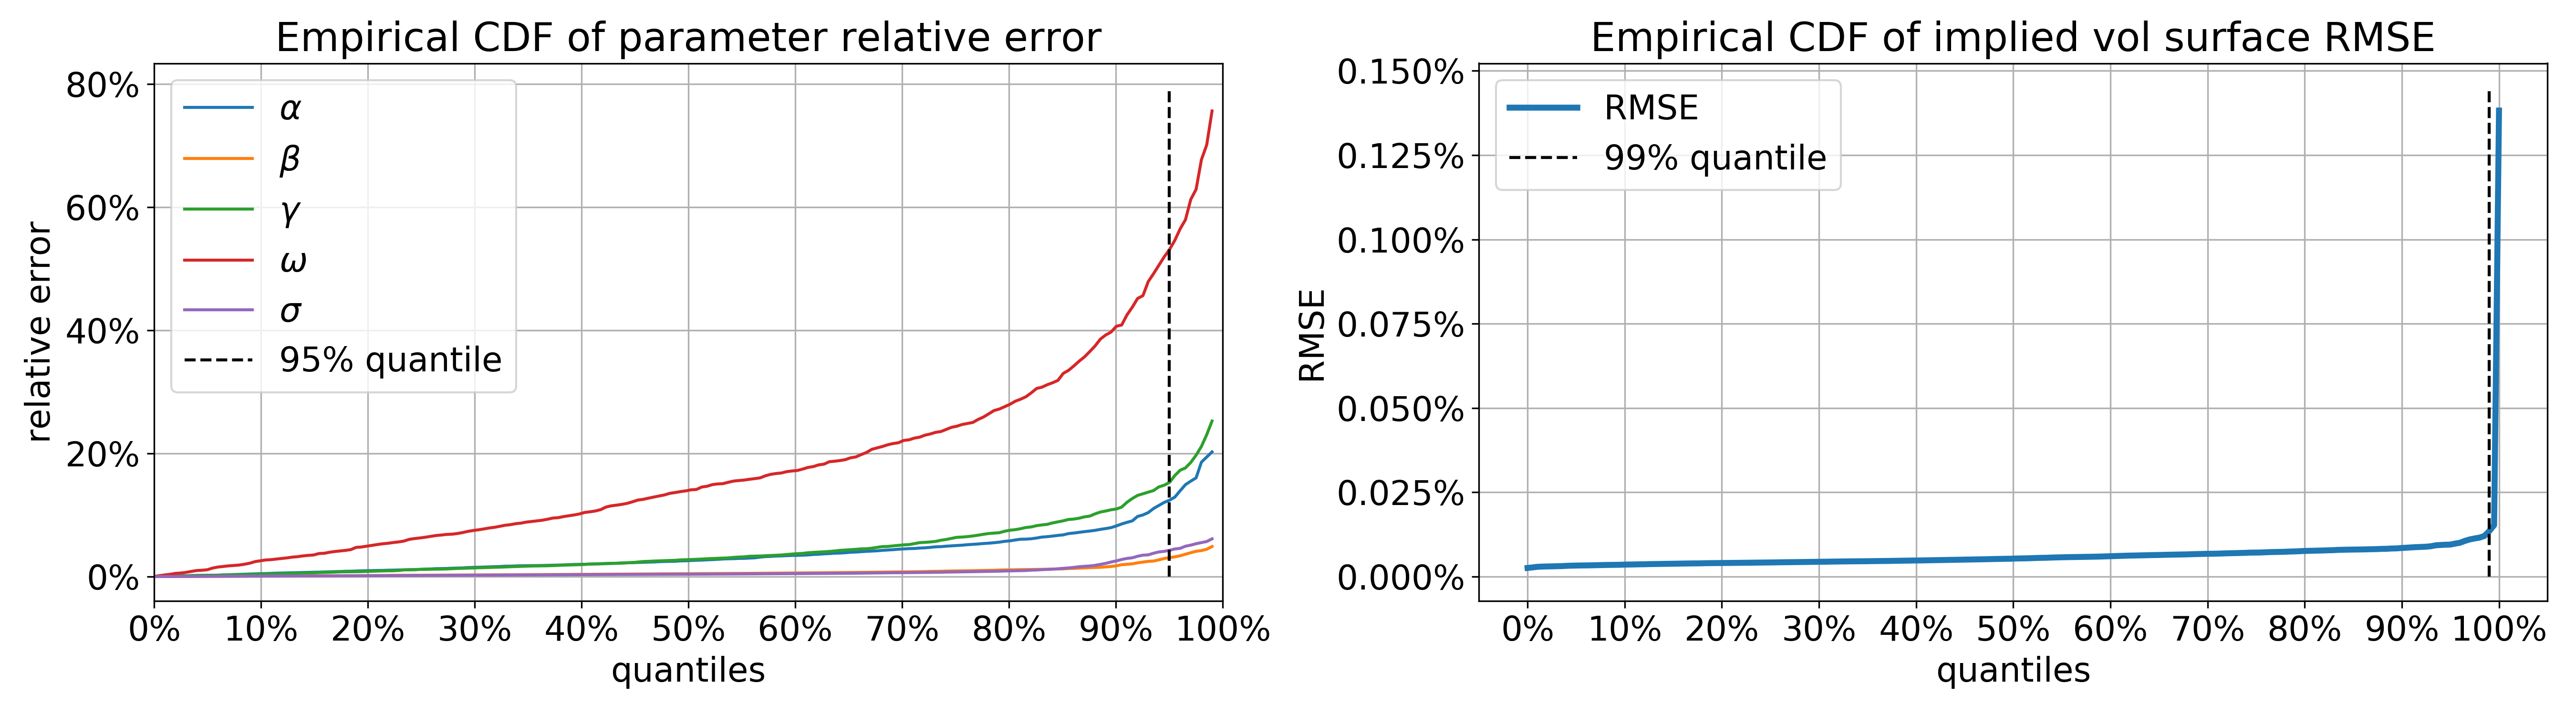
\includegraphics[width=\textwidth]{Small_g_HNG_ErrorCDF.png}
\caption{Best fit - Empirical CDF of parameter relative error and empirical CDF of implied volatility surface RMSE}
\label{fig:small_g_CDF}
\end{figure}
%\fi %zum Auskommentieren
%=========================================================================

%=====
\section{Further Robustness Test}\label{app:robust_size}
This section shows the results of a 20\% reduction of training set size (cf. Section \ref{sec:robust_size})
\begin{table}[!ht]
    \centering
    \begin{tabular}{|r|c|c|c|c|}\hline
     & Layer 1     &  Layer 2     & Layer 3 &    Output\\\hline
    avg. p-val & 4.553e-1&  2.066e-1& 2.701e-1& 1.184e-8***\\\hline
    med. p-val & 4.219e-1 & 1.851e-1 & 1.951e-1& 3.612e-12***\\\hline
    max. p-val & 9.804e-1 & 6.125e-1 &7.318e-1&2.192e-7***\\\hline
    \end{tabular}\vspace{0.1cm}
    \caption{2-Sample-KS-test - Comparison of weights in Neural Nets}
    \label{tab:weights_size_20p}
\end{table}
%=======================
%\iffalse
\begin{figure}[!ht]
    \centering
    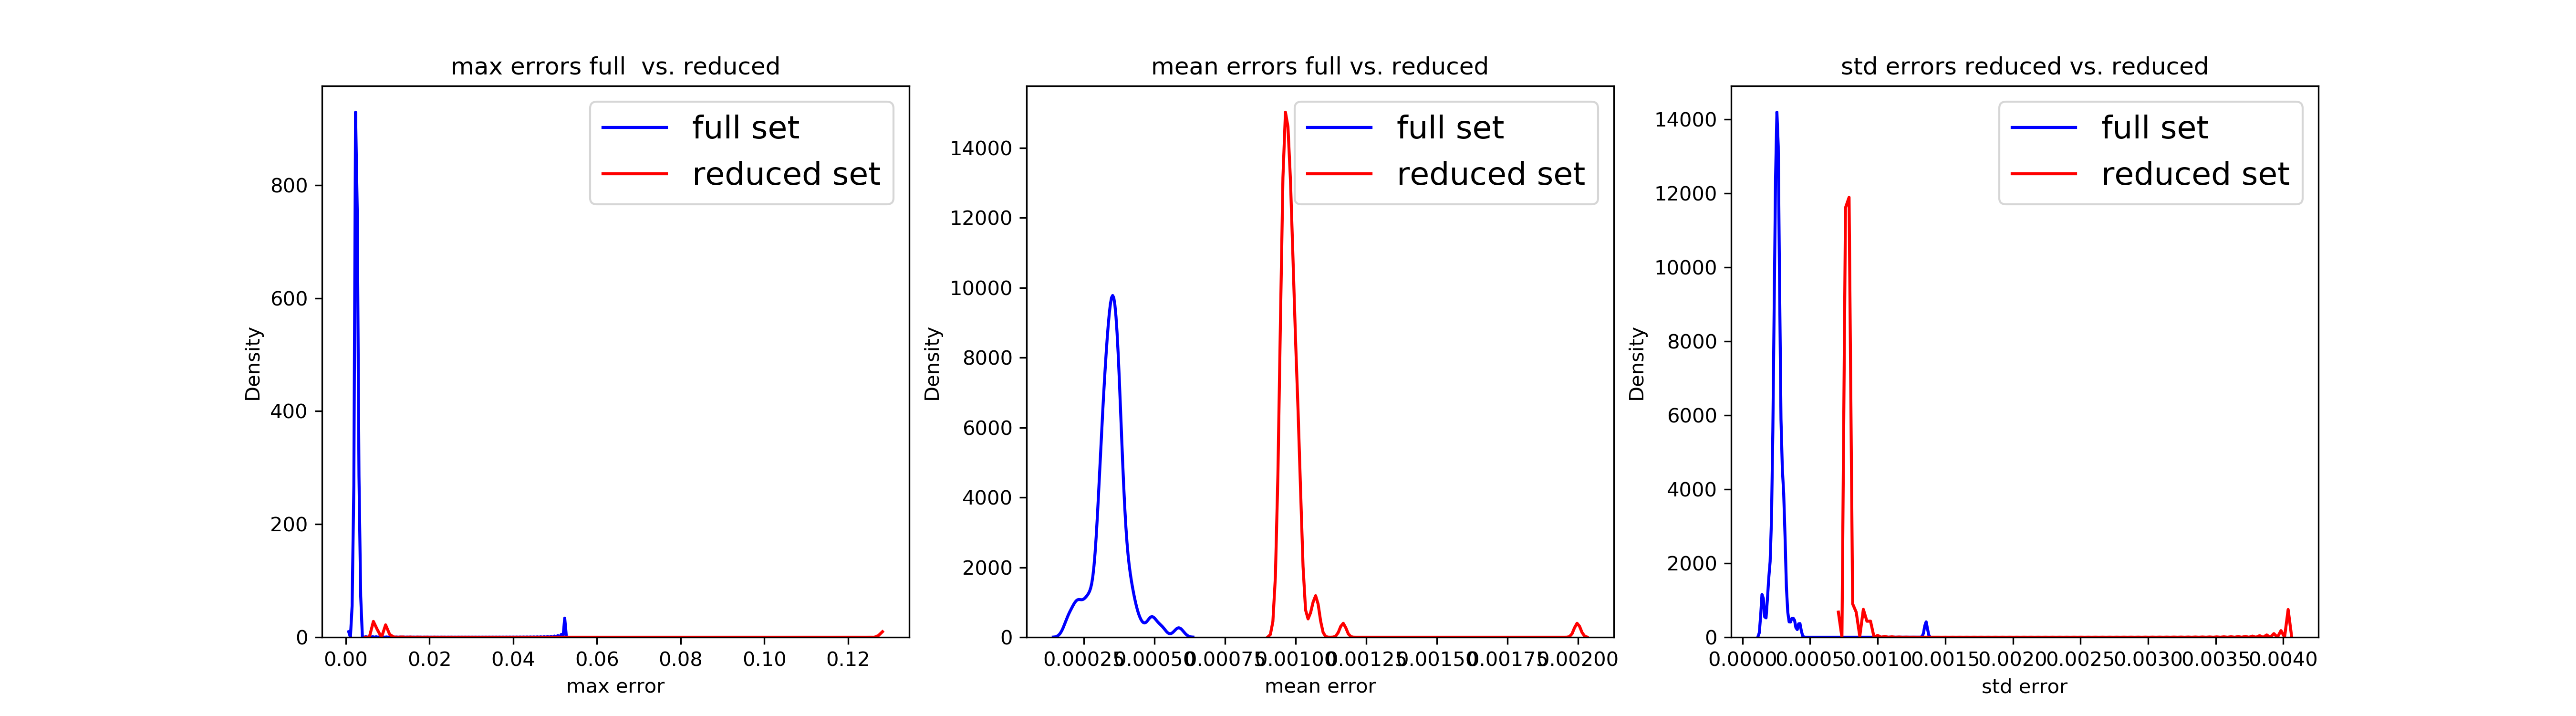
\includegraphics[width=\textwidth]{RobustnessSize20p.png}
    \caption{Robustnesstest - Change in size of training set (20\%)}
    \label{fig:trainset_sensitivity}
\end{figure}
%\fi
%============
\section{Black Scholes Comparison}\label{app:bs_rmse}
This section corresponds to Section \ref{sec:bs_results}.
%\iffalse %======================================
\begin{figure}[!ht]
    \centering
    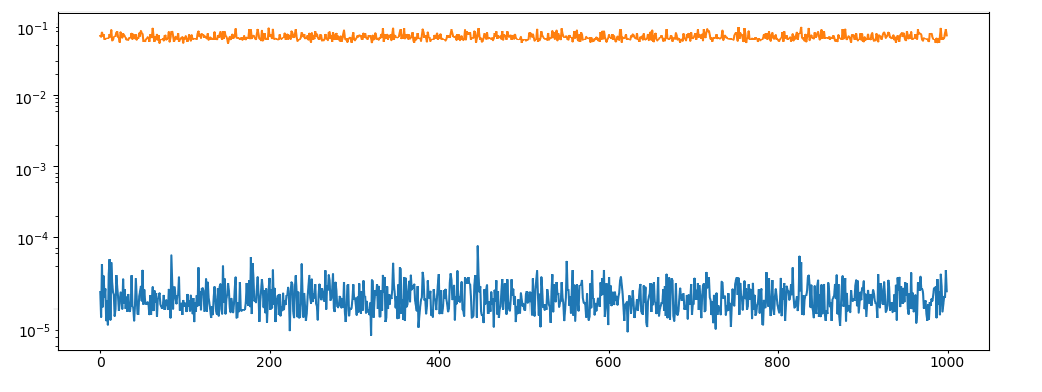
\includegraphics[width=\textwidth]{rmse_modelvsbls.png}
    \caption{RMSE of Neural Net (blue) and Blacks Scholes (orange) on test set }
    \label{fig:rmse_bs_net}
\end{figure}
%\fi
%=========================================

\end{document}